% template presente
\documentclass[a4paper,12pt]{article}

\usepackage{tabularx}
\usepackage{tcolorbox}
\usepackage[utf8]{inputenc}
\usepackage[italian]{babel}
\usepackage{hyperref}
\usepackage{xurl}
\hypersetup{
    colorlinks=true,
    linkcolor=blue,
    filecolor=blue,
    urlcolor=blue,     
}
\usepackage{graphicx}
% Percorsi di ricerca per le immagini
\graphicspath{{resources/}{../resources/}{../../resources/}{../../../resources/}{../../../../resources/}}
\usepackage{xcolor}
\usepackage{geometry}
\usepackage{setspace}
\usepackage{longtable}
\usepackage{colortbl}
\usepackage{fancyhdr}
\usepackage{float} 
\usepackage{enumitem} 
\usepackage{titlesec}
\usepackage{amssymb} 
\usepackage{titlesec}
\usepackage[T1]{fontenc}

\setlength{\headheight}{30pt}

\geometry{margin=2.5cm}

% ===== Variabile per il titolo del documento =====
\newcommand{\documenttitle}{Analisi dei requisiti } 

\setlength{\parindent}{0pt}
\setstretch{1.2}

% ===== Stile intestazione =====
\setlength{\headheight}{33pt}
\pagestyle{fancy}
\fancyhf{}
\fancyhead[L]{\textcolor{gray}{\documenttitle - BitByBit}}
\fancyhead[R]{\includegraphics[height=1cm]{solo_logo.jpg}}
\fancyfoot[C]{\thepage}

% ===== Formattazione sezioni =====
\titleformat{\section}{\Large\bfseries}{\thesection.}{0.5em}{}
\titleformat{\subsection}{\large\bfseries}{\thesubsection.}{0.5em}{}
\titleformat{\subsubsection}{\normalsize\bfseries}{\thesubsubsection}{0.5em}{}

\newcommand{\term}[1]{\textbf{#1}$^\mathbf{G}$}

\newcommand{\ignoreglossary}{}

\begin{document}

% ====== FRONT PAGE ======

\vspace*{5cm}

\begin{center}
    \begin{minipage}{0.25\textwidth}
        \centering
        
\includegraphics[width=\linewidth]{logoUni.png}
    \end{minipage}
    \hfill
    \begin{minipage}{0.7\textwidth}
        \raggedright
        {\color{red}\LARGE \textbf{Università degli Studi di Padova}}\\[0.3cm]
        {\large
        Laurea: Informatica\\
        Corso: Ingegneria del Software\\
        Anno Accademico: 2025/26
        }
    \end{minipage}
\end{center}

\vspace{1cm}

\begin{center}
    \begin{minipage}{0.25\textwidth}
        \centering
        
\includegraphics[width=\linewidth]{logo.png}
    \end{minipage}
    \hfill
    \begin{minipage}{0.7\textwidth}
        \raggedright
        {\LARGE \textbf{Gruppo 17}}\\[0.3cm]
        {\large
        Nome: BitByBit\\
        Email: swe.bitbybit@gmail.com
        }
    \end{minipage}
\end{center}

\vspace{1.5cm}

\begin{center}
    {\LARGE \textbf{\documenttitle}}
\end{center}

\vspace*{\fill}

% ======= INFO GENERALI =======
\renewcommand{\arraystretch}{1.3}

\begin{tcolorbox}
\begin{tabularx}{\textwidth}{@{}l X@{}}
\textbf{Stato:} & Completo\\
\textbf{Versione:} & 1.6.0 \\
\textbf{Responsabile:} & Giovanni Visentin \\
\textbf{Redattori:} & 
\begin{tabular}[t]{@{}l@{}}
Riccardo Manisi\\
Giovanni Visentin\\
Marco Sanguin\\
Dennis Parolin\\
Gabriele Scaggiante\\
Ferdinando Fracasso\\
\end{tabular} \\
\textbf{Verificatori:} & 
\begin{tabular}[t]{@{}l@{}}
Riccardo Manisi\\
Giovanni Visentin\\
Marco Sanguin\\
Dennis Parolin\\
Gabriele Scaggiante\\
Ferdinando Fracasso\\
\end{tabular} \\
\textbf{Destinatari:} &
\begin{tabular}[t]{@{}l@{}}
Miriade srl\\
Prof. Tullio Vardanega\\
Prof. Riccardo Cardin\\
Gruppo BitByBit\\
\end{tabular} \\
\end{tabularx}
\end{tcolorbox}

\vspace*{\fill} 

% ===== REGISTRO MODIFICHE =======
\clearpage
\section*{Registro delle modifiche}
\begin{center}
\small
\renewcommand{\arraystretch}{1.2} 
\arrayrulecolor{black}
\begin{longtable}{|c|c|>{\raggedright\arraybackslash}p{0.21\linewidth}|>{\raggedright\arraybackslash}p{0.23\linewidth}|c|}
\hline
\rowcolor{gray!60} 
\textbf{Versione} & \textbf{Data} & \textbf{Autore} & \textbf{Descrizione} & \textbf{Verificatore} \\
\hline
\rowcolor{gray!20}
1.6.0 & 2026-03-20 & Dennis Parolin & Riscrittura della sezione \hyperref[subsection:requisiti_funzionali]{Requisiti Funzionali} & Gabriele Scaggiante \\
\hline
\rowcolor{white}
1.5.0 & 2026-03-20 & Giovanni Visentin & Riscrittura dei casi d'uso che erano stati segnalati dopo il colloquio con il professore (da \hyperref[sec:UC-44]{UC-44} a \hyperref[subsec:UC-68]{UC-68}). & Dennis Parolin \\
\hline
\rowcolor{gray!20}
1.4.0 & 2026-03-19 & Marco Sanguin & Riscrittura dei casi d'uso per il diario fittizio da \hyperref[subsec:UC-37]{UC-37} a \hyperref[subsec:UC-43]{UC-43}. & Riccardo Manisi \\
\hline
\rowcolor{white}
1.3.0 & 2026-03-18 & Ferdinando Fracasso & Modificati \hyperref[subsec:UC-28]{UC-28}, \hyperref[subsec:UC-29]{UC-29} e \hyperref[subsec:UC-32]{UC-32}, ora da \hyperref[subsec:UC-30]{UC-30} a \hyperref[subsec:UC-36]{UC-36} più sottocasi & Dennis Parolin \\
\hline
\rowcolor{gray!20}
1.2.0 & 2026-03-18 & Gabriele Scaggiante & Riscrittura dei casi d'uso da \hyperref[subsec:UC-21]{UC-21} a \hyperref[subsec:UC-29]{UC-29}. Inserimento nuovi casi \hyperref[subsec:UC-28]{UC-28},\hyperref[subsec:UC-28.1]{UC-28.1},\hyperref[subsec:UC-28.1.1]{UC-28.1.1},\hyperref[subsec:UC-29]{UC-29},\hyperref[subsec:UC-29.1]{UC-29.1},\hyperref[subsec:UC-29.1.1]{UC-29.1.1}. & Riccardo Manisi \\
\hline
\rowcolor{white}
1.1.0 & 2026-03-17 & Dennis Parolin & Riscrittura dei casi d'uso da \hyperref[sec:UC-4]{UC-4} a \hyperref[subsec:UC-13.1]{UC-13.1}. Il caso d'uso \hyperref[sec:UC-5]{UC-5} è stato aggiunto come nuovo caso d'uso. Rifatta tutta la sezione "Requisiti di vincolo" (\ref{subsection:requisiti_vincolo}) e "Requisiti di qualità" (\ref{subsection:requisiti_qualita}). & Riccardo Manisi \\
\hline
\rowcolor{gray!20}
1.0.1 & 2026-03-17 & Riccardo Manisi & Modificati caso d'uso \hyperref[sec:UC-17]{UC-17} e aggiunti sottocasi \hyperref[sec:UC-17.1]{UC-17.1}, \hyperref[sec:UC-17.2]{UC-17.2}  &  Gabriele Scaggiante\\
\hline
\rowcolor{white}
1.0.0 & 2026-03-01 & Giovanni Visentin & Approvazione del documento & Riccardo Manisi \\
\hline
\rowcolor{gray!20}
0.21.0 & 2026-02-27 & Marco Sanguin & Aggiunte immagini per ogni use case, sistemati titoli, frecce e caption tabelle & Dennis Parolin \\
\hline
\rowcolor{white}
0.20.1 & 2026-02-09 & Dennis Parolin & Sistemati errori di compilazione. Sistemate le caption delle tabelle. Sistemati UC-7.1, UC-7.2 e UC-7.3 a cui mancavano le post-condizioni & Giovanni Visentin \\
\hline
\rowcolor{gray!20}
0.20.0 & 2026-02-09 & Dennis Parolin & Riscritta la sezione "Requisiti" (\ref{section:requisiti}) con le sue sottosezioni (\ref{subsection:requisiti_funzionali}, \ref{subsection:requisiti_qualita}, \ref{subsection:requisiti_vincolo}) sulla base dei nuovi casi d'uso redatti. & Giovanni Visentin \\
\hline
\rowcolor{white}
0.19.7 & 2026-02-06 & Dennis Parolin & Modificati i termini ambigui. Aggiunti UC-59 e UC-60 per rimpiazzare UC-9. Sistemati casi d'uso UC-8, UC-8.2, UC-8.3, UC-12, UC-12.2 e UC-12.3 di conseguenza per integrarli con UC-59 e UC-60. & Marco Sanguin \\
\hline
\rowcolor{gray!20}
0.19.6 & 2026-02-05 & Dennis Parolin & Riscritta la sezione Attori (\ref{subsection:attori}) sulla base dei nuovi casi d'uso redatti. Aggiunto l'indice riassuntivo delle tabelle e l'indice riassuntivo delle immagini. & Marco Sanguin \\
\hline
\rowcolor{white}
0.19.5 & 2026-02-02 & Dennis Parolin & Eliminato UC-47. UC-46 è diventato UC-45.1. Aggiunti UC-57 e UC-58. & Marco Sanguin \\
\hline
\rowcolor{gray!20}
0.19.4 & 2026-01-27 & Giovanni Visentin & Aggiunta casi d'uso \term{Walkthrough} & Gabriele Scaggiante \\
\hline
\rowcolor{white}
0.19.3 & 2026-01-16 & Gabriele Scaggiante & Rinominazione codici casi d'uso & Giovanni Visentin \\
\hline
\rowcolor{gray!20}
0.19.2 & 2026-01-16 & Giovanni Visentin & Aggiunta casi d'uso dead man switch & Gabriele Scaggiante \\
\hline
\rowcolor{white}
0.19.1 & 2026-01-16 & Giovanni Visentin & Aggiunta casi d'uso guida & Gabriele Scaggiante \\
\hline
\rowcolor{gray!20}
0.19.0 & 2026-01-15 & Gabriele Scaggiante & Aggiunti UC Guardiano Silenzioso & Giovanni Visentin \\
\hline
\rowcolor{white}
0.18.2 & 2026-01-15 & Gabriele Scaggiante & Corretti alcuni refusi & Giovanni Visentin \\
\hline
\rowcolor{gray!20}
0.18.1 & 2026-01-15 & Gabriele Scaggiante & Aggiunti scenari secondari negli UC del diario & Giovanni Visentin \\
\hline
\rowcolor{white}
0.18.0 & 2026-01-15 & Giovanni Visentin & Riscritti gli UC per chatbot e cronologia chat (da terminare) & Gabriele Scaggiante \\
\hline
\rowcolor{gray!20}
0.17.0 & 2026-01-14 & Gabriele Scaggiante & Riscritti gli UC per il diario secondo il nuovo schema & Giovanni Visentin \\
\hline
\rowcolor{white}
0.16.1 & 2026-01-13 & Ferdinando Fracasso & Aggiunta nella sezione "Attori" & Dennis Parolin \\
\hline
\rowcolor{gray!20}
0.16.0 & 2026-01-12 & Giovanni Visentin & Inizio riscrittura UC secondo nuovo schema & Dennis Parolin \\
\hline
\rowcolor{white}
0.15.4 & 2026-01-12 & Ferdinando Fracasso & Correzione errori nelle sezioni "Attori" e "Requisiti" & Dennis Parolin \\
\hline
\rowcolor{gray!20}
0.15.3 & 2026-01-11 & Ferdinando Fracasso & Aggiunta sezione requisiti & Dennis Parolin \\
\hline
\rowcolor{white}
0.15.2 & 2026-01-09 & Ferdinando Fracasso & Modifica sezione attori nei casi d'uso & Dennis Parolin \\
\hline
\rowcolor{gray!20}
0.15.1 & 2025-12-23 & Dennis Parolin & Aggiunte le immagini dei diagrammi UML riguardanti i casi d'uso & Giovanni Visentin \\
\hline
\rowcolor{white}
0.14.0 & 2025-12-22 & Giovanni Visentin & Modifica UC-IMP8 in IMP9 e aggiunti UC-I & Dennis Parolin \\
\hline
\rowcolor{gray!20}
0.13.0 & 2025-12-21 & Giovanni Visentin & Aggiunto caso d'uso UC-IMP8 e proposto UC-SYS1 & Dennis Parolin \\
\hline
\rowcolor{white}
0.12.0 & 2025-12-19 & Riccardo Manisi & Aggiunta UC-D1, UC-D2 per impostazione e modifica password diario criptato. Eliminato UC-BW1.6 [deprecato] & Dennis Parolin \\
\hline
\rowcolor{gray!20}
0.11.0 & 2025-12-19 & Riccardo Manisi &  Inseriti casi d'uso per autenticazione all'app UC-AUTH1 e UC-AUTH1.1. Cancellato UC-BW1.5 [deprecato] & Giovanni Visentin \\
\hline
\rowcolor{white}
0.10.0 & 2025-12-17 & Riccardo Manisi & Cancellato UC-BW1.5 [deprecato] in UC-BW1 e inserita inclusione con UC-IMP3 & Giovanni Visentin \\
\hline
\rowcolor{gray!20}
0.9.0 & 2025-12-16 & Marco Sanguin & Aggiunti Casi d'uso per Guardiano Silenzioso e Detective delle Relazioni (UC-S, UC-I) & Giovanni Visentin \\ 
\hline
\rowcolor{white}
0.8.1 & 2025-12-16 & Dennis Parolin & Sistemato errore di una sezione ripetuta due volte ma con una sottosezione differente & Marco Sanguin \\
\hline
\rowcolor{gray!20}
0.8.0 & 2025-12-15 & Giovanni Visentin & Aggiunti casi d'uso per Diari fittizio (UC-D4, UC-D5, UC-D5.1, UC-23.1) & Marco Sanguin \\
\hline
\rowcolor{white}
0.7.0 & 2025-12-12 & Riccardo Manisi & Aggiunti casi d'uso per schermata impostazioni (UC-IMP1) e quelli relativi ai contatti fidati & Giovanni Visentin \\
\hline
\rowcolor{gray!20}
0.6.0 & 2025-12-12 & Dennis Parolin & Rifacimento completo casi d'uso Benvenuto e \term{Walkthrough} (UC-BW) & Marco Sanguin\\
\hline
\rowcolor{white}
0.5.0 & 2025-12-11 & Riccardo Manisi & Prima stesura casi d'uso \term{Walkthrough} & Giovanni Visentin \\
\hline
\rowcolor{gray!20}
0.4.0 & 2025-12-11 & Riccardo Manisi & Aggiunta sezione scopo dei casi d'uso, attori e nomenclatura per casi d'uso & Giovanni Visentin \\
\hline
\rowcolor{white}
0.3.0 & 2025-12-11 & Dennis Parolin & Redazione della sezione \ref{sec:funzioni_prodotto}. Modifica sezione \ref{sec:prospettiva_prodotto} sulla base delle funzionalità concordate con la \term{Proponente}. Spostato il registro delle modifiche a prima dell'indice. & Giovanni Visentin \\
\hline
\rowcolor{gray!20}
0.2.0 & 2025-12-11 & Dennis Parolin & Redazione delle sezioni \ref{sec:scopo_documento}, \ref{sec:prospettiva_prodotto}, \ref{sec:riferimenti}, \ref{sec:riferimenti_normativi} e \ref{sec:riferimenti_informativi} & Marco Sanguin \\
\hline
\rowcolor{white}
0.1.0 & 2025-12-10 & Riccardo Manisi & Creazione del documento & Giovanni Visentin \\
\hline
\end{longtable}
\end{center}

\clearpage

% Indice dei contenuti
\tableofcontents
\thispagestyle{empty}

\clearpage

% Indice delle tabelle
\listoftables

% Indice delle figure
\listoffigures

\clearpage

% ======= INTRODUZIONE ========

\section{Introduzione}
\subsection{Scopo del documento} \label{sec:scopo_documento}
Il presente documento di \term{Analisi Dei Requisiti} ha l'obiettivo di esporre in modo esaustivo e non ambiguo le specifiche funzionali, prestazionali e vincolanti del sistema software oggetto di sviluppo.

L'analisi qui condotta si basa sull'identificazione dei Casi d'Uso (Use Cases), supportati dai relativi diagrammi UML, utilizzati per modellare le interazioni previste tra gli attori e il sistema. Tale approccio permette di derivare puntualmente i requisiti software finali.

Questo elaborato costituisce il riferimento primario per le successive fasi del \term{Ciclo Di Vita} del software, guidando la progettazione architetturale, l'implementazione del codice e le attività di \term{Verifica} e \term{Validazione}. Ciò garantisce che il prodotto finale sia conforme alle aspettative e alle necessità espresse dal \term{Proponente}.

I requisiti individuati sono stati prioritizzati secondo la seguente classificazione:
\begin{itemize}
    \item \textbf{Obbligatori:} requisiti essenziali e bloccanti, necessari per il funzionamento base del sistema;
    \item \textbf{Desiderabili:} requisiti che offrono un valore aggiunto significativo, pur non essendo strettamente indispensabili nell'immediato;
    \item \textbf{Opzionali:} requisiti di utilità marginale o posticipabili a sviluppi futuri.
\end{itemize}

Il documento, redatto dagli Analisti del gruppo \textit{BitByBit}, è destinato ai seguenti \term{Stakeholder}:
\begin{itemize}
    \item \textbf{\term{Committente}/\term{Proponente}:} per la \term{Validazione} delle specifiche e la conferma che i requisiti siano stati recepiti correttamente;
    \item \textbf{Team di Sviluppo (Progettisti e Programmatori):} come linea guida tecnica per la realizzazione del prodotto;
    \item \textbf{Verificatori:} come base per la definizione dei piani di test e per la \term{Verifica} della conformità del software.
\end{itemize}

% =======================PROSPETTIVA PRODOTTO================================

\subsection{Prospettiva del prodotto} \label{sec:prospettiva_prodotto}
Il prodotto che il gruppo \textit{BitByBit} si prefigge di realizzare è un'applicazione mobile multipiattaforma (Android e iOS) denominata "L'app che Protegge e Trasforma". Il sistema si colloca in un dominio critico e sensibile, con l'obiettivo primario di prevenire la violenza di genere (focalizzandosi principalmente su donne tra i 18 e i 30 anni) e fornire supporto concreto attraverso strumenti di consapevolezza e sicurezza.

A differenza di una tradizionale applicazione informativa, il sistema integra funzionalità \textbf{attive e intelligenti}, ma con un approccio etico definito: l'Intelligenza Artificiale non agisce autonomamente in situazioni critiche, ma funge da supporto analitico ("Detective delle relazioni" e "Specchio intelligente") per aiutare l'\term{Utente} a decodificare la propria situazione e riconoscere pattern di rischio. Le funzionalità di allerta verso i contatti fidati ("Guardiano Silenzioso") o di emergenza rimangono sempre vincolate a un'attivazione esplicita dell'\term{Utente} o a controlli di inattività, evitando automatismi rischiosi da parte dell'IA.

La prospettiva del sistema si estende oltre la singola interazione, offrendo un hub informativo ("Guida al coraggio") che collega l'\term{Utente} a risorse esterne, normative e mappe di luoghi sicuri. Data la natura dei dati trattati, il prodotto pone un vincolo architetturale imprescindibile sulla \textbf{sicurezza e la privacy}: il sistema garantisce funzionalità di offuscamento (camuffamento icona), crittografia dei contenuti personali (Diario criptato) e gestione granulare della rete di supporto.

Infine, il sistema è progettato per essere affidabile e accessibile in contesti duali: sia come strumento di prevenzione riflessiva in momenti di calma, sia come supporto rapido e intuitivo in condizioni di stress o difficoltà, scalando le risorse per future integrazioni (es. widget o microservizi).

% =======================FUNZIONALITA' PRODOTTO================================

\subsection{Funzioni del prodotto} \label{sec:funzioni_prodotto}

Il prodotto dovrà seguire le seguenti funzionalità principali:

\begin{itemize}
    \item Welcome page e \term{Walkthrough} introduttivo;
    \item Pagina impostazioni;
    \item Login e gestione Account;
    \item Detective delle relazioni;
    \item Lo specchio intelligente;
    \item La guida al coraggio;
    \item Guardiano silenzioso;
    \item Diario criptato.
\end{itemize}

\subsubsection{Welcome Page e \ignoreglossary{Walkthrough}}
L'esperienza \ignoreglossary{utente} avrà inizio con una schermata di benvenuto volta a comprendere la finalità dell'installazione. Tale interfaccia presenterà due opzioni: "Per me" o "Per altri". Questa distinzione è fondamentale per fornire un contesto iniziale al Large Language Model (LLM) e preconfigurare determinati parametri. Inoltre, tale struttura permetterà in futuro l'implementazione di funzionalità differenziate in base al beneficiario del servizio.

Successivamente, sarà proposto un \term{Walkthrough} illustrativo delle funzionalità disponibili. È prevista la presenza di un comando per saltare tale guida, permettendo l'accesso diretto alle funzionalità dell'app.

\subsubsection{Account e Impostazioni}
È prevista l'implementazione di una sezione per la gestione dell'account. L'\term{Utente} avrà la facoltà di fornire un indirizzo e-mail personale, utilizzabile per l'invio di notifiche qualora si rilevi un periodo prolungato di inattività, fungendo da meccanismo di controllo (dead man's switch) per verificare lo stato di sicurezza dell'\term{Utente} o l'abbandono volontario dell'app.

Un'ulteriore sezione sarà dedicata alle preferenze, incluse la gestione della rete di contatti fidati, la personalizzazione delle notifiche e la scelta dell'icona dell'app (funzionalità di "camuffamento" per proteggere la privacy in caso di \term{Ispezione} del dispositivo da parte di terzi) e delle informazioni condivisibili (es. posizione geografica). La configurazione della rete di supporto è cruciale: l'\term{Utente} potrà inserire e-mail o numeri di telefono di persone ritenute \textbf{fidate}, dati essenziali per il funzionamento del \textbf{Guardiano Silenzioso}. Tale funzionalità è progettata per essere scalabile, prevedendo in futuro l'invio di diverse tipologie di notifiche.

\subsubsection{Detective delle Relazioni e Lo Specchio Intelligente}
L'interfaccia includerà una sezione dedicata all'interazione testuale con l'Intelligenza Artificiale, concepita per chiarire dubbi e fornire supporto. Questa schermata implementerà due distinte funzionalità: \textbf{Detective delle relazioni} e \textbf{Lo specchio intelligente}.
La prima ha l'obiettivo di analizzare comportamenti o narrazioni dell'\term{Utente} per identificare la situazione attuale e riconoscere pattern di pericolo meritevoli di attenzione. La seconda è orientata all'autoconsapevolezza, offrendo uno spazio privato per l'analisi dei propri pensieri.
La selezione del prompt più adeguato tra i due sarà gestita automaticamente dall'app previa analisi del messaggio \term{Utente}, mantenendo comunque la possibilità di modifica manuale. È prevista inoltre una sezione per l'archiviazione delle chat, consentendone la consultazione e la prosecuzione futura.

\subsubsection{La Guida al Coraggio}
La sezione denominata \textbf{La guida al coraggio} fungerà da hub informativo, offrendo accesso chiaro a risorse essenziali. I contenuti includeranno:
\begin{itemize}
    \item Link a siti web di riferimento;
    \item Link a materiale video educativo;
    \item Collegamenti a forum di discussione esistenti;
    \item Definizioni normative e informazioni sulla "violenza di genere";
    \item Informazioni legali (diritti, azioni permesse, procedure di denuncia, ecc.).
\end{itemize}
Sarà inoltre integrata una mappa per la visualizzazione dei "luoghi sicuri", con indicazioni sui percorsi per raggiungerli basate sulla geolocalizzazione dell'\term{Utente} (tramite integrazione con Google Maps).

\subsubsection{Guardiano Silenzioso}
Tale funzionalità è concepita per l'invio tempestivo di comunicazioni di emergenza (e-mail o SMS) ai contatti della rete di supporto in caso di pericolo o necessità. L'attivazione di tali comunicazioni non sarà demandata all'IA, ma sarà gestita direttamente dall'\term{Utente} tramite un comando "\textbf{SOS}" chiaramente visibile e di rapido accesso.

Qualora il dispositivo si trovi in condizioni di scarsa o nulla connettività internet, l'applicazione prevede una modalità di sicurezza ausiliaria. In tale scenario, previo comando specifico dell'\term{Utente}, verrà attivato un allarme acustico volto ad attirare l'attenzione dei presenti e dissuadere eventuali aggressori.

\subsubsection{Diario Criptato}
Il \textbf{Diario Criptato} costituirà uno spazio sicuro per l'annotazione di eventi, pensieri e l'archiviazione di file multimediali (foto e audio). L'accesso a tale sezione sarà protetto da password o autenticazione biometrica, e l'interfaccia sarà progettata per essere discreta.

A tutela della sicurezza dell'\term{Utente} in situazioni di costrizione, è previsto un meccanismo di accesso differenziato: qualora l'\term{Utente} sia forzato a mostrare il contenuto del diario, l'inserimento di una password errata darà accesso a un diario fittizio. Questa versione conterrà elementi coerenti e sensati, ma privi di qualsiasi informazione sensibile. L'inserimento della password corretta, invece, garantirà il normale accesso al diario reale e ai dati personali archiviati.

In una prima fase, il diario non sarà interconnesso con l'IA.
Tuttavia, l'\term{Architettura} è predisposta per future estensioni, eventualmente sviluppate da team specializzati o tramite microservizi. Possibili evoluzioni includono l'analisi dei contenuti del diario da parte dell'IA per arricchire il contesto delle conversazioni, o viceversa, l'esportazione automatica delle chat nel diario. Si ipotizza inoltre l'implementazione di widget per smartphone o smartwatch per l'inserimento rapido di note vocali o fotografiche.

% =======================CARATTERISTICHE \term{Utente}================================

\subsection{Caratteristiche dell'\ignoreglossary{Utente}} \label{sec:caratteristiche utente}
A seguito dell'analisi dei potenziali fruitori, il target primario dell'applicazione è stato identificato nelle donne nella fascia d'età compresa tra i 18 e i 30 anni. Tuttavia, il sistema è progettato per accogliere anche utenti esterni interessati a reperire informazioni sul tema.

L'interazione con il sistema varia significativamente in base al contesto d'uso, spaziando dalla ricerca informativa alla necessità di supporto rapido. Si identificano le seguenti tipologie principali di attori:

\begin{itemize}
    \item \textbf{\term{Utente} Target (Donne 18-30 anni):} È l'utilizzatore principale. L'applicativo si configura primariamente come strumento di prevenzione; lo scenario ideale prevede che l'\term{Utente} interagisca con l'app avendo tempo a disposizione (es. per informarsi o valutare la propria situazione in un contesto di calma apparente).
    Tuttavia, il sistema deve garantire supporto anche in situazioni di difficoltà e stress (es. potenziale violenza domestica). Va specificato che, in caso di pericolo di vita imminente, si presuppone che la vittima contatti direttamente le autorità (es. 118), bypassando l'applicazione.
    
    \item \textbf{Rete di Supporto e Terze Parti:} Questa categoria eterogenea include la cerchia amicale (contatti fidati scelti dall'\term{Utente}), i professionisti del settore (es. psicologi) e gli utenti esterni. Questi attori interagiscono con il sistema per fornire supporto, ricevere notifiche o, nel caso degli utenti esterni, consultare la sezione informativa dedicata.
\end{itemize}

In conclusione, il sistema deve essere accessibile a utenti con competenze tecniche variabili, garantendo usabilità sia durante la consultazione approfondita (fase di prevenzione) sia in momenti in cui l'\term{Utente} necessita di un aiuto rapido e discreto (fase di stress), pur non sostituendosi ai servizi di emergenza primaria.

% ====== RIFERIMENTI ======

\subsection{Riferimenti} \label{sec:riferimenti}


% ====== DEFINIZIONI, ACRINIMI E ABBREVIAZIONI ======

Al fine di evitare ambiguità relative al linguaggio e ai termini utilizzati all'interno dei documenti formali, viene allegato il \href{https://swe-bitbybit.github.io/SWE-docs/docs/RTB/documenti_interni/Glossario.pdf}{\textit{Glossario}}.
I termini tecnici, gli acronimi e le parole con significato specifico all'interno del progetto sono contrassegnati da una lettera 'G' in apice (es. Agile\textsuperscript{G}) e sono descritti in dettaglio nel documento apposito.

\subsubsection{Riferimenti normativi}\label{sec:riferimenti_normativi}
\begin{itemize}
\item \textbf{\term{Capitolato} d'appalto C4: \emph{L'app che Protegge e Trasforma}}\\
Parti consultate: documento completo\\
Versione: 1.0\\
Ultimo accesso: \textit{2026-01-14}\\
\url{https://www.math.unipd.it/~tullio/IS-1/2025/Progetto/C4.pdf}

\pagebreak %---Inserito perchè altrimenti il riferimento successivo viene tagliato in due

\item \textbf{Norme di Progetto}\\
Parti consultate: documento completo\\
Versione: v.1.0.0\\
Ultimo accesso: \textit{2026-02-09}\\
\url{https://swe-bitbybit.github.io/SWE-docs/docs/RTB/documenti_interni/norme_di_progetto.pdf} %---Link del sito, ma non funziona al momento---
\end{itemize}

\subsubsection{Riferimenti informativi} \label{sec:riferimenti_informativi}
\begin{itemize}
    \item \textbf{Standard IEEE 830 1998}\\
        Parti consultate: documento completo\\
        Versione: \textit{edizione 1998}\\
        Ultimo accesso: \textit{2026-01-13}\\
        \url{https://ieeexplore.ieee.org/document/720574}
    \item \textbf{Standard ISO/IEC 12207:1995}\\
        Parti consultate: documento completo\\
        Versione: \textit{edizione 1997} \\
        Ultimo accesso: \textit{2026-01-13}\\
        \url{https://www.math.unipd.it/~tullio/IS-1/2009/Approfondimenti/ISO_12207-1995.pdf}
    \item \textbf{Slide sull'\emph{\term{Analisi Dei Requisiti}} del Prof. Vardanega}\\
        Parti consultate: documento completo\\
        Versione: \textit{A.A.2025/2026}\\
        Ultimo accesso: \textit{2026-01-13}\\
        \url{https://www.math.unipd.it/~tullio/IS-1/2025/Dispense/T05.pdf}
    \item \textbf{Slide sui \emph{diagrammi dei casi d'uso} del Prof. Cardin}\\
        Parti consultate: documento completo\\
        Versione: \textit{A.A.2025/2026}\\
        Ultimo accesso: \textit{2026-01-13}\\
        \url{https://www.math.unipd.it/~rcardin/swea/2022/Diagrammi%20Use%20Case.pdf}
    \item \textbf{\emph{\term{Repository} Github} del Prof. Cardin}\\
        Ultimo accesso: \textit{2026-01-13}\\
        \url{https://github.com/rcardin/swe-imdb}
    \item \textbf{Glossario}\\
        Parti consultate: documento completo\\
        Versione: \textit{v.1.0.0}\\
        Ultimo accesso: \textit{2026-02-27}\\
        \url{https://swe-bitbybit.github.io/SWE-docs/docs/RTB/documenti_interni/Glossario.pdf}
\end{itemize}

% ---------------------------- SEZIONE CASI D'USO -------------------------------

\section{Casi d'uso}

\subsection{Scopo}
Nel \term{Processo} di analisi, come indicato nel documento delle Norme di progetto, il gruppo \textbf{BitByBit} ha stabilito come prima attività l'individuazione dei casi d'uso del sistema. La stesura dei casi d'uso costituisce uno strumento fondamentale per la successiva individuazione dei requisiti funzionali del sistema, poiché consentono di definire in modo chiaro all'\term{Utente} come il sistema sarà impiegato per soddisfare specifici obiettivi.\\
Nello specifico essi rappresentano una descrizione di come il sistema interagisce con i suoi attori per raggiungere un obiettivo specifico.
Ogni caso d'uso ha uno scenario principale che rappresenta il flusso standard di interazioni e può includere scenari alternativi che fanno arrivare il sistema in uno stato diverso da quello che si identifica nello scenario principale del caso.\\
Per facilitare la comprensione da parte dei lettori sia tecnici che non, alla descrizione in linguaggio naturale, viene anche associato un diagramma UML, che offre una rappresentazione grafica delle interazioni tra attori e sistema.\\
Per ogni caso d'uso presentato in questo documento viene adottata una struttura uniforme. I termini specifici adottati sono raccolti nella sezione dedicata (\hyperref[nomenclatura-casi-duso]{Sezione~\ref*{nomenclatura-casi-duso}}).

\subsection{Nomenclatura casi d'uso}
\label{nomenclatura-casi-duso}
Questa sezione raccoglie i termini tecnici specifici utilizzati nella descrizione dei casi d’uso presenti in questo documento.

\begin{center}
\small
\arrayrulecolor{black} 
\begin{longtable}{|p{0.30\textwidth}|p{0.60\textwidth}|}

\hline
\rowcolor{gray!60}
{\centering \textbf{Termine}\par} &
{\centering \textbf{Descrizione}\par} \\
\hline
\rowcolor{white}
\centering \textbf{Attore principale} & Attore che interagisce attivamente con il sistema. \\
\hline
\rowcolor{gray!20}
\centering \textbf{Attore secondario} & Coloro che interagiscono passivamente con il sistema. \\
\hline
\rowcolor{white}
\centering \textbf{Pre-condizioni} & Lista di elementi o condizioni che sono necessari affinché l'attore possa eseguire gli scenari del caso d'uso. \\
\hline
\rowcolor{gray!20}
\centering \textbf{Post-condizioni} & Condizioni che devono essere vere al termine dell'esecuzione del caso d'uso. Descrivono lo stato finale osservabile del sistema dopo la conclusione del caso d'uso.  \\
\hline
\rowcolor{white}
\centering \textbf{Scenario principale} & Sequenza di passi che descrive il flusso standard del caso d'uso. Rappresenta l'happy path dell'esecuzione del caso d'uso che conduce al raggiungimento dell'obiettivo fissato. \\
\hline
\rowcolor{gray!20}
\centering \textbf{Scenario secondario} & Sequenza di passi che devia dallo scenario principale a seguito di condizioni particolari. Porta il sistema in condizioni diverse da quelle dello scenario principale. \\
\hline
\rowcolor{white}
\centering \textbf{Inclusioni} & Relazione tra casi d'uso in cui il caso d'uso incluso viene eseguito in modo incondizionato durante i passi del caso d'uso principale. \\
\hline
\rowcolor{gray!20}
\centering \textbf{Estensioni} & Relazione tra casi d'uso in cui il caso d'uso esteso viene eseguito solo quando si verificano le condizioni di estensione definite. \\
\hline
\rowcolor{white}
\centering \textbf{Specializzazioni} & Relazione di generalizzazione tra casi d'uso in cui uno o più casi d'uso derivati ereditano comportamento, precondizioni e post-condizioni da un caso d'uso generale, introducendo eventuali variazioni o raffinamenti specifici. \\
\hline
\rowcolor{gray!20}
\centering \textbf{Trigger} & Evento o condizione che avvia l'esecuzione del caso d'uso. \\
\hline

\caption{Tabella nomenclatura casi d'uso} \label{tab:nomenclatura} \\

\end{longtable}
\end{center}

\subsection{Attori} \label{subsection:attori}
Gli attori sono entità esterne che interagiscono con il sistema per raggiungere determinati obiettivi. Essi si distinguono in due categorie principali:
\begin{itemize}
    \item \textbf{Attori principali:} sono coloro che avviano attivamente l'interazione con il sistema per soddisfare un proprio bisogno o scopo.
    \item \textbf{Attori secondari:} sono entità (spesso sistemi esterni o servizi) che partecipano all'interazione fornendo dati o servizi necessari al sistema, ma senza avviare direttamente il caso d'uso. Spesso sono attori passivi.
\end{itemize}
Di seguito vengono rappresentati quali attori primari e secondari sono stati utilizzati:
\begin{figure}[H]
    \centering
    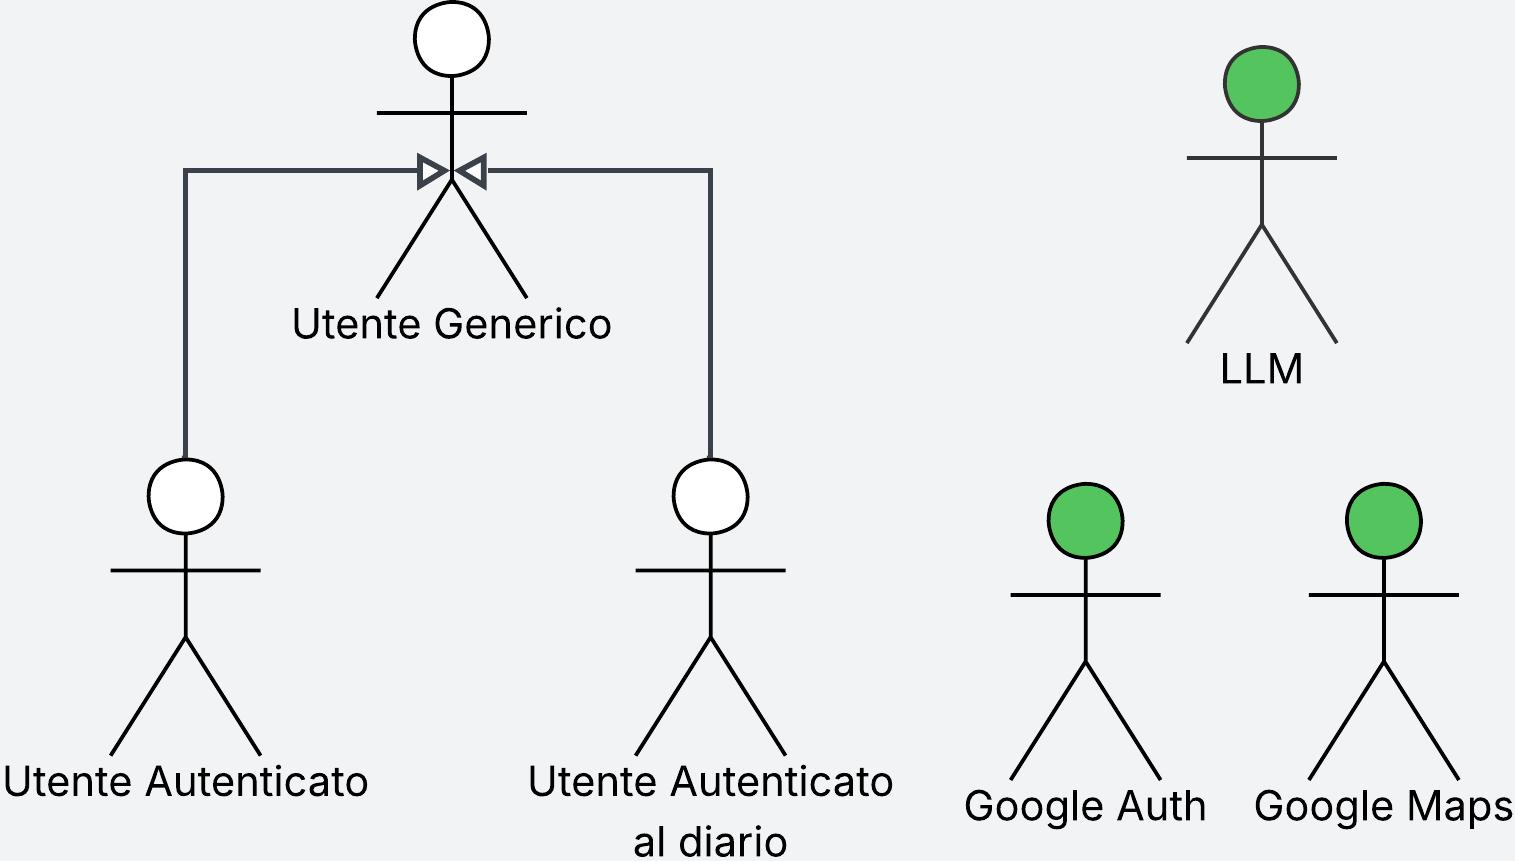
\includegraphics[width=1\textwidth]{attori.png}
    \caption{Diagramma degli attori}
    \label{fig:attori}
\end{figure}

\begin{center}
\small
\arrayrulecolor{black}
\begin{longtable}{|p{0.30\textwidth}|p{0.60\textwidth}|}

\hline
\rowcolor{gray!70}
\centering \textbf{Attori primari} & \centering \textbf{Descrizione} \tabularnewline
\hline
\endfirsthead
\hline
\endhead
\rowcolor{white}
\centering \textbf{\term{Utente} Generico} & Un \term{Utente} che non ha eseguito l'autenticazione all'applicazione e che non ha ancora creato una password per il diario criptato. Il sistema permette a questo attore di eseguire un sottoinsieme della totalità delle funzionalità. \\
\hline
\rowcolor{gray!20}
\centering \textbf{\term{Utente} Autenticato} & Un \term{Utente} il quale ha eseguito l'autenticazione all'applicazione. Il sistema possiede l'indirizzo mail di questo attore. Ha accesso a delle funzionalità aggiuntive rispetto all'\term{Utente} Generico e all'\term{Utente} autenticato al diario. \\
\hline
\rowcolor{white}
\centering \textbf{\term{Utente} autenticato al diario} & \term{Utente} che ha impostato la password per il diario criptato. \\
\hline
\rowcolor{gray!70}
\centering \textbf{Attori secondari} & \centering \textbf{Descrizione} \tabularnewline
\hline
\rowcolor{white}
\centering \textbf{Google Auth} & Servizio di autenticazione esterno che permette al sistema di identificare l'\term{Utente} tramite le proprie credenziali Google, evitando la creazione di nuovi account dedicati. \\
\hline
\rowcolor{gray!20}
\centering \textbf{Google Maps} & Servizio di mappatura esterno invocato dal sistema per mostrare la posizione precisa dei luoghi sicuri e calcolare i percorsi per raggiungerli. \\
\hline
\rowcolor{white}
\centering \textbf{LLM} & Modello di Intelligenza Artificiale esterno che riceve i messaggi dell'\term{Utente} e il contesto della conversazione per generare risposte coerenti e simulare un'interazione umana nelle funzionalità di supporto. \\
\hline

\caption{Tabella di spiegazione degli attori} \label{tab:attori} \\

\end{longtable}
\end{center}

% ===== LISTA CASI D'USO ======

\subsection{Lista casi d'uso}

% ==== AUTENTICAZIONE APP ====

\subsubsection{UC-1 Autenticazione all'app tramite Google Auth} \label{subsec:UC-1}

\begin{figure}[H]
    \centering
    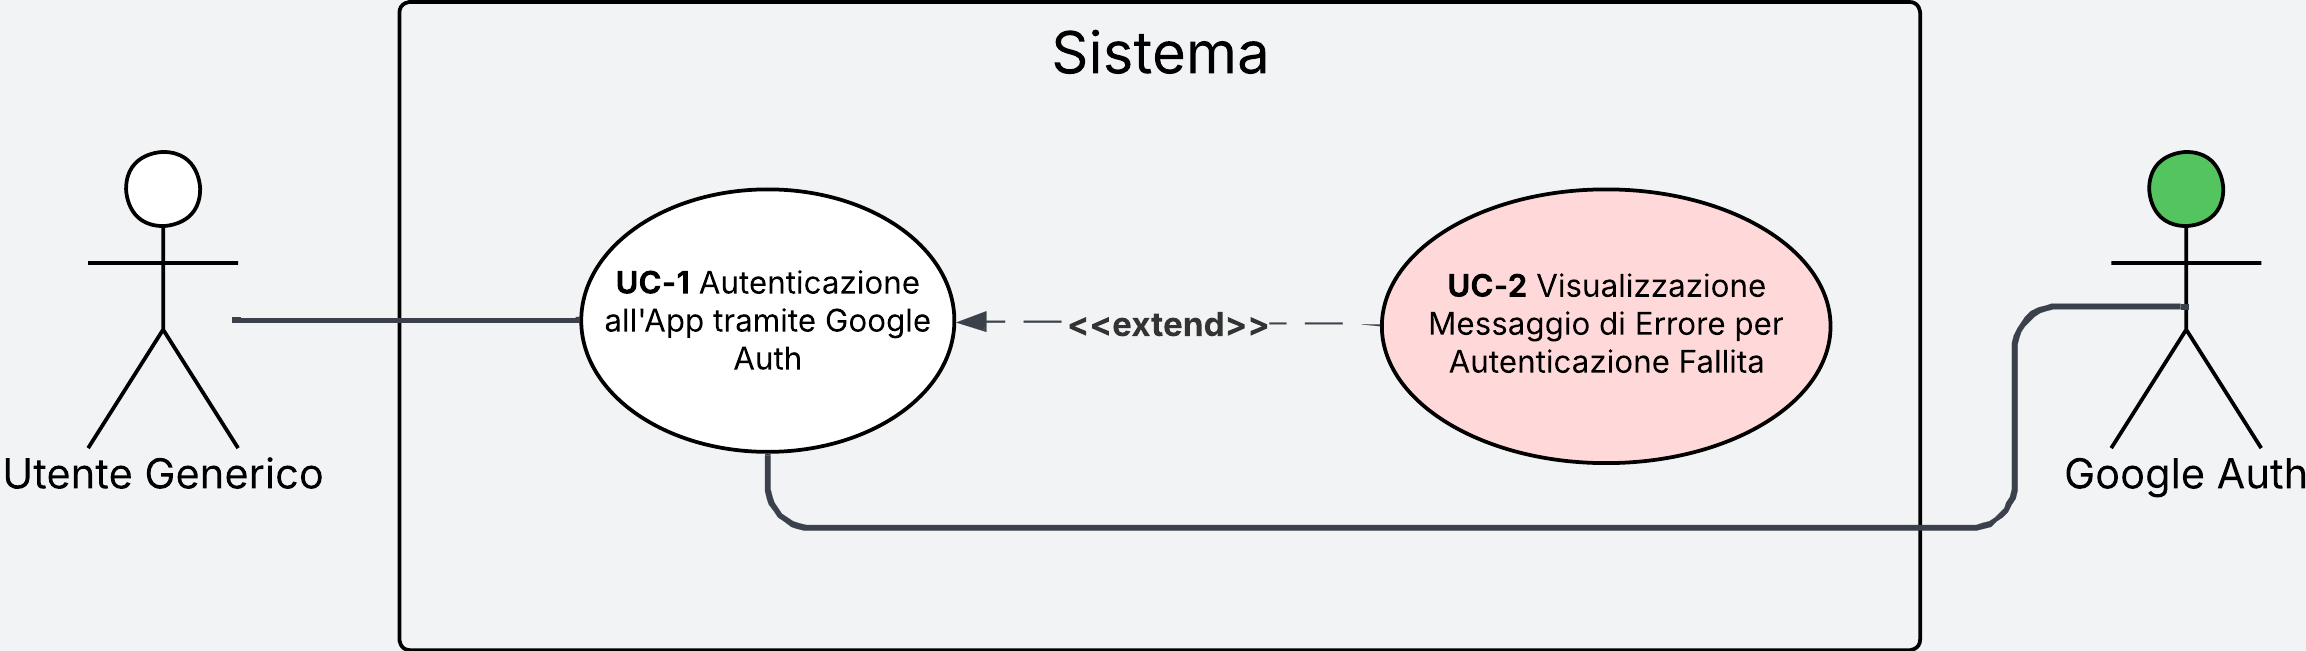
\includegraphics[width=1\textwidth]{use_case/UC-1-auth.png}
    \caption{Diagramma del caso d'uso UC-1}
    \label{fig:UC-1}
\end{figure}

\begin{itemize}
    \item \textbf{Attore principale:} \term{Utente} Generico
    \item \textbf{Attore secondario:} Google Auth
    \item \textbf{Pre-condizioni:} 
    \begin{itemize}
        \item Il sistema è attivo
        \item L'attore non è autenticato all'applicazione
    \end{itemize}
    \item \textbf{Post-condizioni:}
    \begin{itemize}
        \item L’attore è autenticato all'applicazione
        \item Il sistema riconosce l'attore come \term{Utente} Autenticato
        \item L'attore può accedere alle funzionalità riservate dell'applicazione
        \item La funzionalità di Dead Man Switch viene attivata automaticamente
    \end{itemize}
    \item \textbf{Scenario principale:}
    \begin{itemize}
        \item L'attore richiede l'autenticazione tramite Google
        \item L'attore viene reindirizzato a Google Auth dal sistema
        \item L'attore si autentica su Google Auth
        \item L'attore accede al sistema come "\term{Utente} Autenticato"
    \end{itemize}
    \item \textbf{Scenario secondario:}
    \begin{itemize}
        \item Google Auth restituisce errore $\rightarrow$ \hyperref[subsec:UC-2]{UC-2}
    \end{itemize} 
    \item \textbf{Estensioni:}
    \begin{itemize}
        \item \hyperref[subsec:UC-2]{UC-2}
    \end{itemize}
    \item \textbf{Trigger:} L'attore vuole accedere all'applicazione
\end{itemize}

\subsubsection{UC-2 Visualizzazione messaggio di errore per autenticazione fallita} \label{subsec:UC-2}
\begin{itemize}
    \item \textbf{Attore principale:} \term{Utente} Generico
    \item \textbf{Attore secondario:} Google Auth
    \item \textbf{Pre-condizioni:} 
    \begin{itemize}
        \item Il sistema è attivo
        \item L'attore ha tentato l'autenticazione tramite il servizio Google Auth
        \item Google Auth ha restituito un token non valido o un errore
    \end{itemize}
    \item \textbf{Post-condizioni:}
    \begin{itemize}
        \item L'attore visualizza l'errore
        \item L'autenticazione può essere ripetuta
        \item L'attore rimane nello stato di "\term{Utente} non autenticato"
    \end{itemize}
    \item \textbf{Scenario principale:}
    \begin{itemize}
        \item Il servizio Google Auth comunica al sistema l’esito negativo dell’autenticazione
        \item Il sistema mostra all’attore un messaggio di errore relativo all’autenticazione fallita
    \end{itemize}
    \item \textbf{Trigger:} Google Auth restituisce un codice di errore durante il \ignoreglossary{processo} di autenticazione
\end{itemize}

% ==== UC-3 - SWITCH MODE ====

\subsubsection{UC-3 - Selezione profilo} \label{subsec:UC-3}
\begin{figure}[H]
    \centering
    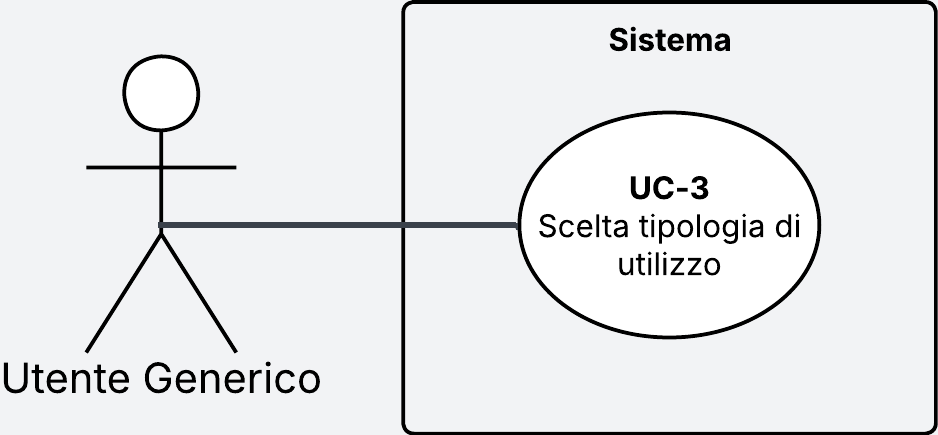
\includegraphics[width=1\textwidth]{use_case/UC-3-switchmode.png}
    \caption{Diagramma del caso d'uso UC-3}
    \label{fig:UC-3}
\end{figure}
\begin{itemize}
    \item \textbf{Attore principale:} \term{Utente} Generico
    \item \textbf{Pre-condizioni:}
    \begin{itemize}
        \item Il sistema è attivo
        \item Sta avvenendo il primo accesso al sistema da parte dell'attore
    \end{itemize}
    \item \textbf{Post-condizioni:}
    \begin{itemize}
        \item Il profilo è salvato dal sistema
    \end{itemize}
    \item \textbf{Scenario principale:}
    \begin{itemize}
        \item L'attore vede una spiegazione della differenza tra i due profili
        \item L'attore visualizza i due profili proposti "Per me" e "Per altri"
        \item L'attore seleziona il profilo "Per me" o "Per altri"
        \item Il sistema salva il profilo scelto
    \end{itemize}
    \item \textbf{Trigger:} Il sistema richiede la selezione del profilo
\end{itemize}

% ==== UC-4 - LISTA CONTATTI FIDATI ====

\subsubsection{UC-4 - Visualizzazione lista contatti fidati} \label{sec:UC-4}
\begin{tcolorbox}[colback=gray!10,colframe=gray!50,title=Nota]
{\small Il caso d'uso \hyperref[sec:UC-4]{UC-4} è suddiviso nei casi d'uso inclusi \hyperref[subsec:UC-4.1]{UC-4.1} e \hyperref[subsec:UC-4.1.1]{UC-4.1.1}, che ne dettagliano il comportamento.
Il diagramma riportato di seguito mostra anche un ulteriore caso d'uso correlato (\hyperref[sec:UC-5]{UC-5}), la cui descrizione dettagliata è riportata nelle sezioni successive del documento.}
\end{tcolorbox}
\begin{figure}[H]
    \centering
    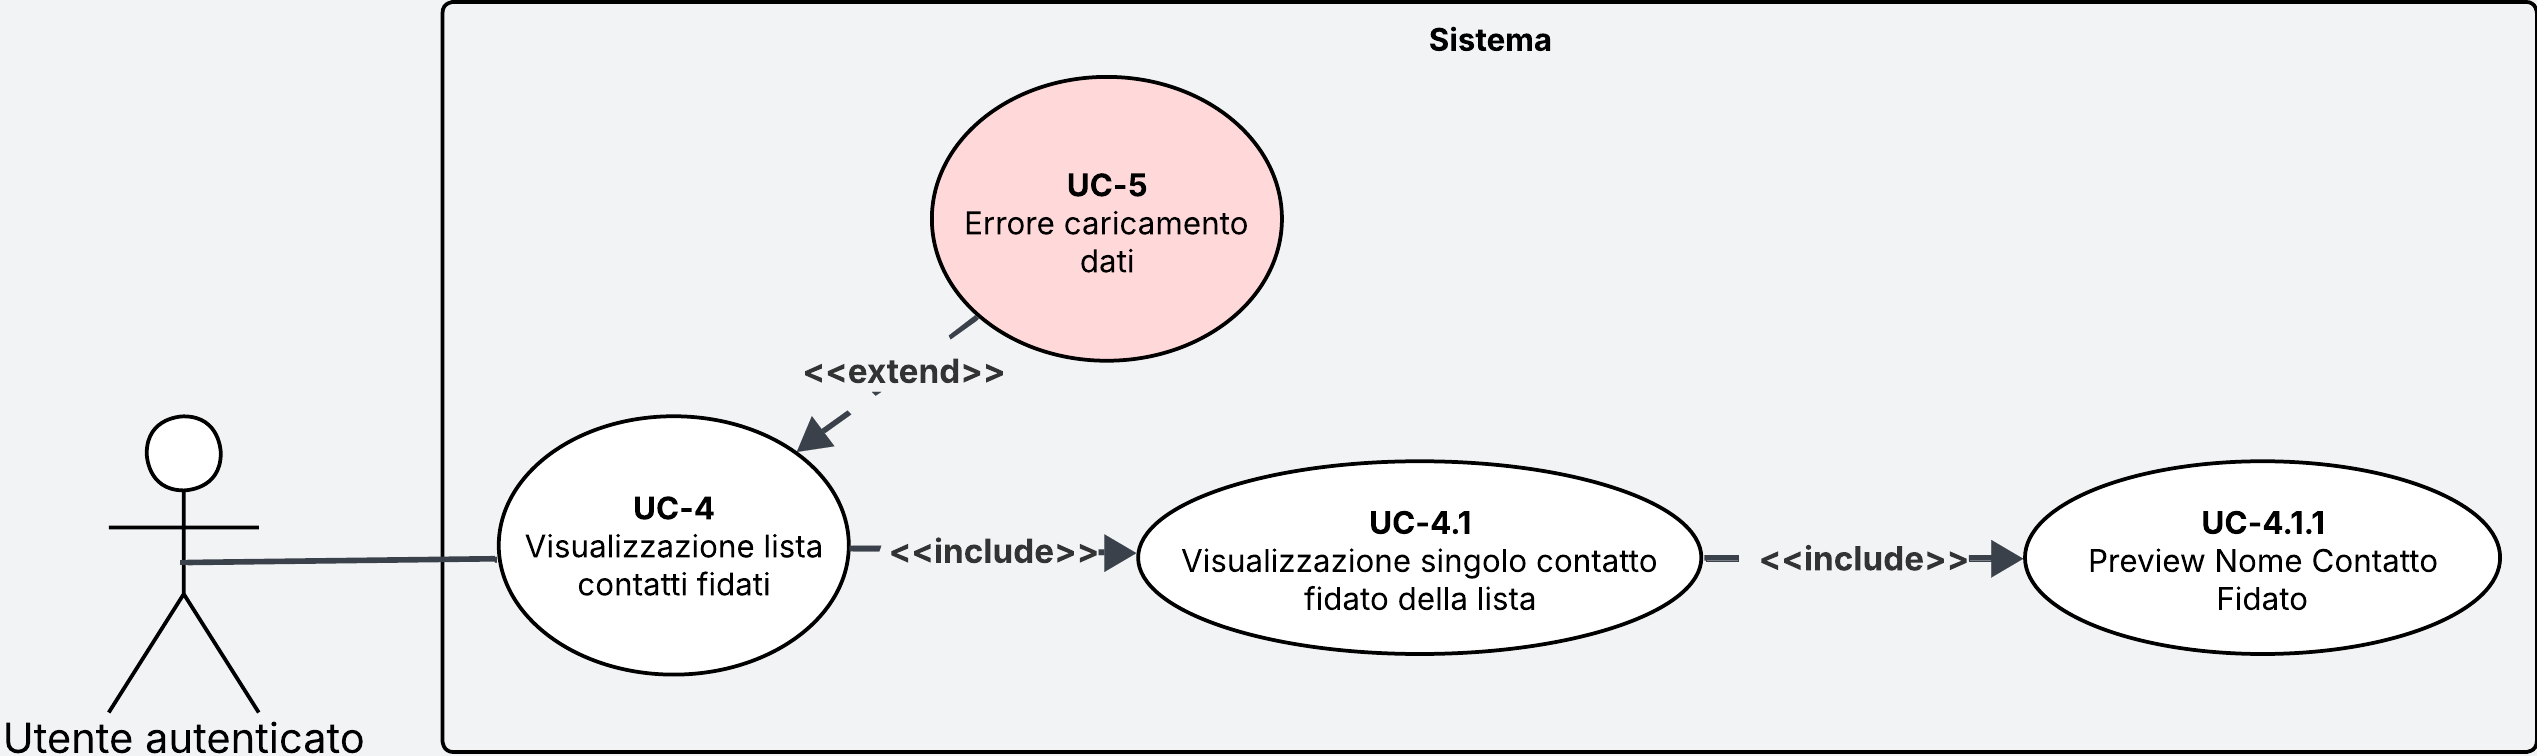
\includegraphics[width=1\textwidth]{use_case/UC-4-lista-contatti-fidati.png}
    \caption{Diagramma del caso d'uso UC-4 con relativi sottocasi d'uso}
    \label{fig:UC-4}
\end{figure}
\begin{itemize}
    \item \textbf{Attore principale:} \term{Utente} Autenticato
    \item \textbf{Pre-condizioni:}
    \begin{itemize}
        \item Il sistema è attivo
        \item L'attore ha selezionato la voce per visualizzare la propria rete di contatti fidati
    \end{itemize}
    \item \textbf{Post-condizioni:} 
    \begin{itemize}
        \item L'attore visualizza la lista dei contatti fidati
    \end{itemize}
    \item \textbf{Scenario principale:} 
    \begin{itemize}
        \item L'attore visualizza le voci della lista dei contatti fidati
        \item L'attore guarda singolarmente i contatti fidati (e la preview delle informazioni del contatto) nella lista, senza interagirvi
    \end{itemize}
    \item \textbf{Scenario secondario:} 
    \begin{itemize}
        \item Si \ignoreglossary{verifica} un errore
        \item Il sistema notifica l'errore all'attore $\rightarrow$ \hyperref[sec:UC-5]{UC-5}
    \end{itemize}
    \item \textbf{Inclusioni:} 
    \begin{itemize}
        \item \hyperref[subsec:UC-4.1]{UC-4.1}
    \end{itemize}
    \item \textbf{Estensioni:} 
    \begin{itemize}
        \item \hyperref[sec:UC-5]{UC-5}
    \end{itemize}
    \item \textbf{Trigger:} L'attore vuole vedere la sua rete dei contatti fidati
\end{itemize}

\subsubsection{UC-4.1 - Visualizzazione singolo contatto fidato della lista} \label{subsec:UC-4.1}
\begin{itemize}
    \item \textbf{Attore principale:} \term{Utente} Autenticato
    \item \textbf{Pre-condizioni:} 
    \begin{itemize}
        \item Il sistema è attivo
        \item L'attore sta visualizzando la lista dei contatti fidati
    \end{itemize}
    \item \textbf{Post-condizioni:}
    \begin{itemize}
        \item L'attore visualizza un singolo contatto dalla lista
    \end{itemize}
    \item \textbf{Scenario principale:} 
    \begin{itemize}
        \item L'attore visualizza un singolo contatto fidato nella lista
        \item L'attore visualizza l'anteprima del nome del contatto fidato $\rightarrow$ \hyperref[subsec:UC-4.1.1]{UC-4.1.1}
    \end{itemize}
    \item \textbf{Inclusioni:}
    \begin{itemize}
        \item \hyperref[subsec:UC-4.1.1]{UC-4.1.1}
    \end{itemize}
    \item \textbf{Trigger:} L'attore vuole visualizzare un singolo contatto fidato dalla lista
\end{itemize}

\subsubsection{UC-4.1.1 - Preview nome contatto fidato} \label{subsec:UC-4.1.1}
\begin{itemize}
    \item \textbf{Attore principale:} \term{Utente} Autenticato
    \item \textbf{Pre-condizioni:}
    \begin{itemize}
        \item Il sistema è attivo
        \item L'attore sta visualizzando la lista dei contatti fidati
        \item L'attore visualizza un singolo contatto dalla lista
    \end{itemize}
    \item \textbf{Post-condizioni:}
    \begin{itemize}
        \item L'attore visualizza l'anteprima del nome del contatto fidato
    \end{itemize}
    \item \textbf{Scenario principale:} 
    \begin{itemize}
        \item L'attore visualizza l'anteprima del nome del singolo contatto fidato dalla lista
    \end{itemize}
\end{itemize}

\subsubsection{UC-5 - Errore caricamento dati} \label{sec:UC-5}

\begin{itemize}
    \item \textbf{Attore principale:} \term{Utente} Generico
    \item \textbf{Pre-condizioni:}
    \begin{itemize}
        \item Il sistema è attivo
        \item L'attore ha selezionato una sezione che prevede il recupero di dati dal database
    \end{itemize}
    \item \textbf{Post-condizioni:} 
    \begin{itemize}
        \item Il sistema notifica l'errore all'attore
    \end{itemize}
    \item \textbf{Scenario principale:} 
    \begin{itemize}
        \item Si \ignoreglossary{verifica} un errore
        \item Il sistema rileva il fallimento della richiesta a causa dell'errore
        \item Il sistema mostra un messaggio di errore all'attore
    \end{itemize}
    \item \textbf{Trigger:} Si \ignoreglossary{verifica} un errore durante il caricamento dei dati
\end{itemize}

\subsubsection{UC-6 - Visualizzazione informazioni contatto fidato} \label{subsec:UC-6}
\begin{tcolorbox}[colback=gray!10,colframe=gray!50,title=Nota]
{\small Il caso d'uso \hyperref[subsec:UC-6]{UC-6} è suddiviso nei casi d'uso inclusi \hyperref[subsec:UC-6.1]{UC-6.1}, \hyperref[subsec:UC-6.2]{UC-6.2} e \hyperref[subsec:UC-6.3]{UC-6.3}, che ne dettagliano il comportamento}
\end{tcolorbox}
\begin{figure}[H]
    \centering
    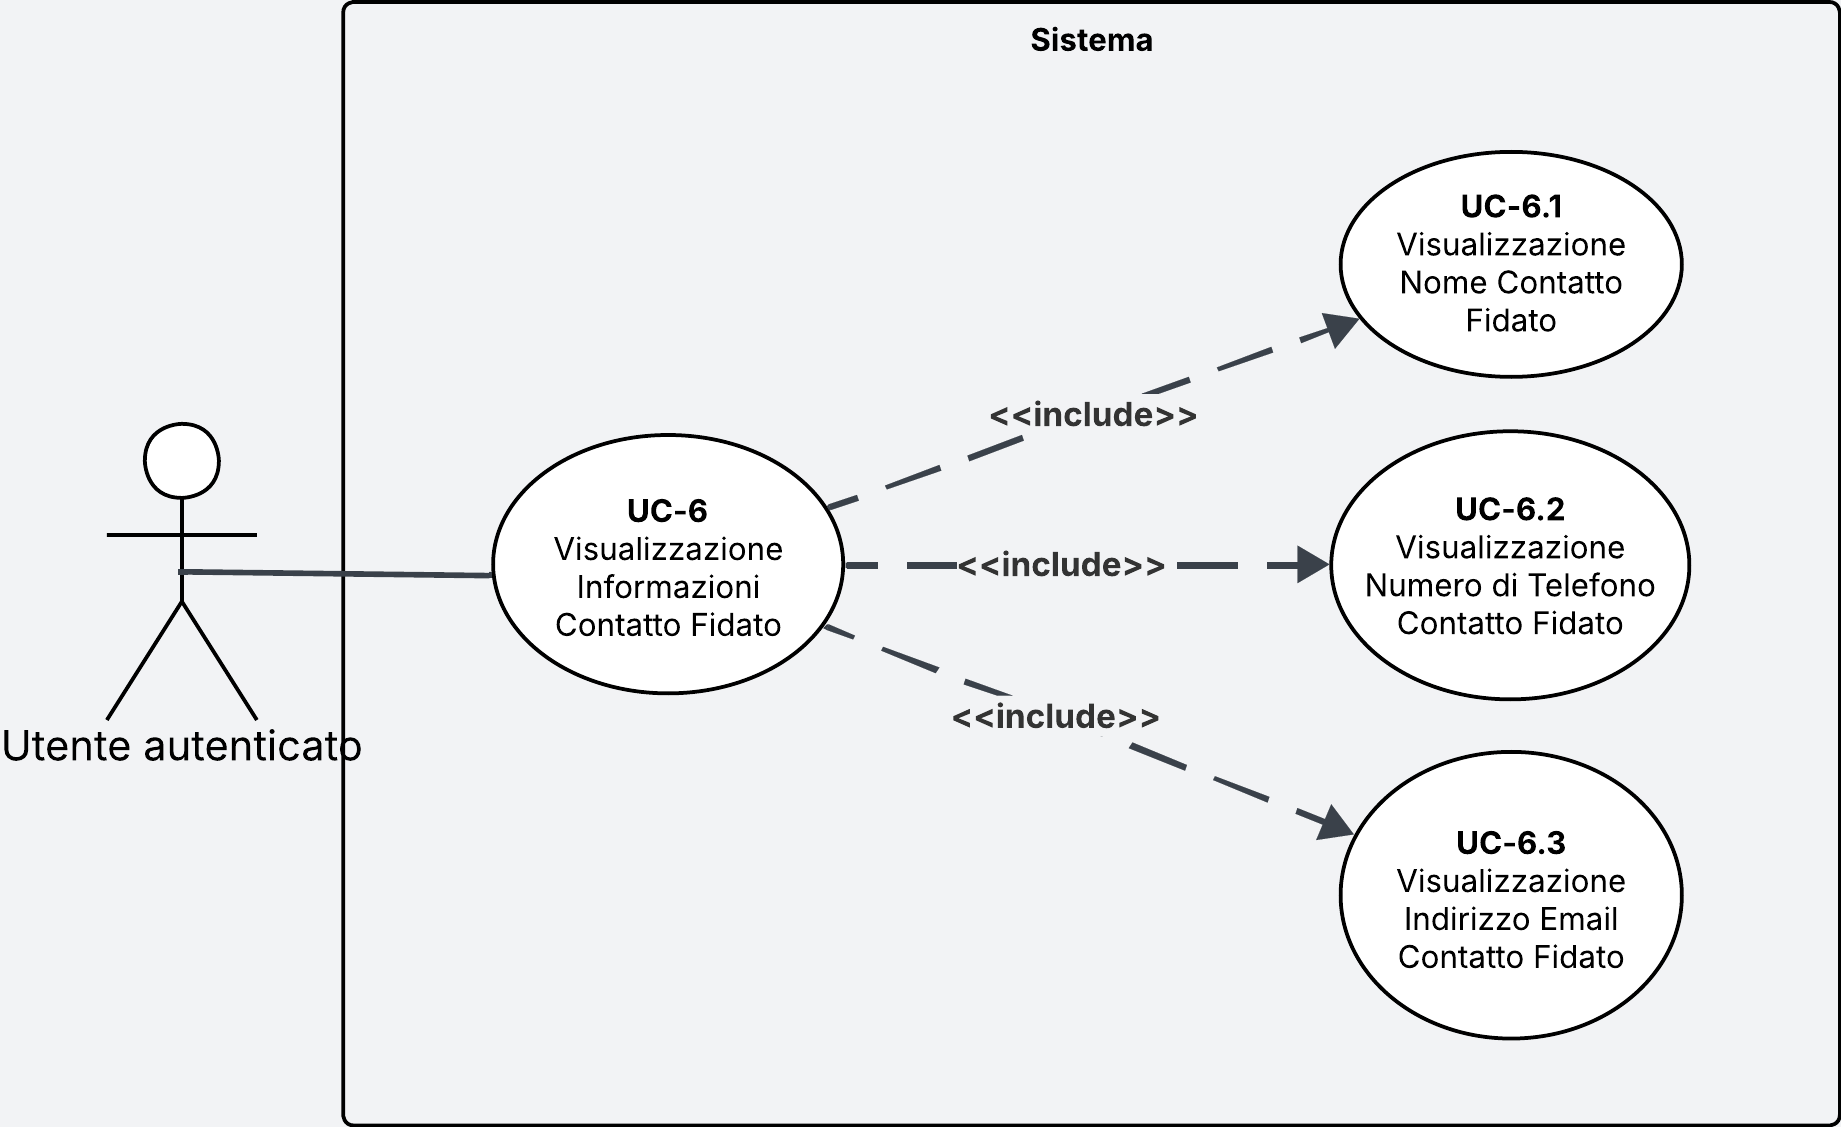
\includegraphics[width=1\textwidth]{use_case/UC-6-visualizzazione-info-contatti-fidati.png}
    \caption{Diagramma del caso d'uso UC-6 con relativi sottocasi d'uso}
    \label{fig:UC-6}
\end{figure}
\begin{itemize}
    \item \textbf{Attore principale:} \term{Utente} Generico
    \item \textbf{Pre-condizioni:} 
    \begin{itemize}
        \item Il sistema è attivo
        \item L'attore sta visualizzando la lista dei contatti fidati
        \item L'attore ha selezionato un contatto fidato dalla lista dei contatti fidati
    \end{itemize}
    \item \textbf{Post-condizioni:}
    \begin{itemize}
        \item L'attore visualizza le informazioni del contatto fidato
    \end{itemize}
    \item \textbf{Scenario principale:} 
    \begin{itemize}
        \item Per il contatto fidato selezionato il sistema mostra le relative informazioni quali:
        \begin{itemize}
            \item il nome $\rightarrow$ \hyperref[subsec:UC-6.1]{UC-6.1}
            \item il numero di telefono $\rightarrow$ \hyperref[subsec:UC-6.2]{UC-6.2}
            \item l'indirizzo email $\rightarrow$ \hyperref[subsec:UC-6.3]{UC-6.3}
        \end{itemize}
    \end{itemize}
    \item \textbf{Inclusioni:}
    \begin{itemize}
        \item \hyperref[subsec:UC-6.1]{UC-6.1}
        \item \hyperref[subsec:UC-6.2]{UC-6.2}
        \item \hyperref[subsec:UC-6.3]{UC-6.3}
    \end{itemize}
    \item \textbf{Trigger:} L'attore vuole visualizzare le informazioni di contatto per un contatto fidato
\end{itemize}

\subsubsection{UC-6.1 - Visualizzazione nome contatto fidato} \label{subsec:UC-6.1}
\begin{itemize}
    \item \textbf{Attore principale:} \term{Utente} Generico
    \item \textbf{Pre-condizioni:} 
    \begin{itemize}
        \item Il sistema è attivo
        \item L'attore sta visualizzando le informazioni del contatto fidato
    \end{itemize}
    \item \textbf{Post-condizioni:}
    \begin{itemize}
        \item L'attore visualizza il nome del contatto fidato
    \end{itemize}
    \item \textbf{Scenario principale:} 
    \begin{itemize}
        \item Il sistema mostra a schermo il nome del contatto fidato
    \end{itemize}
\end{itemize}

\subsubsection{UC-6.2 - Visualizzazione numero di telefono contatto fidato} \label{subsec:UC-6.2}
\begin{itemize}
    \item \textbf{Attore principale:} \term{Utente} Generico
    \item \textbf{Pre-condizioni:} 
    \begin{itemize}
        \item Il sistema è attivo
        \item L'attore sta visualizzando le informazioni del contatto fidato
    \end{itemize}
    \item \textbf{Post-condizioni:}
    \begin{itemize}
        \item L'attore visualizza il numero di telefono del contatto fidato
    \end{itemize}
    \item \textbf{Scenario principale:} 
    \begin{itemize}
        \item Il sistema mostra a schermo il numero di telefono del contatto fidato
    \end{itemize}
\end{itemize}

\subsubsection{UC-6.3 - Visualizzazione indirizzo email contatto fidato} \label{subsec:UC-6.3}
\begin{itemize}
    \item \textbf{Attore principale:} \term{Utente} Generico
    \item \textbf{Pre-condizioni:} 
    \begin{itemize}
        \item Il sistema è attivo
        \item L'attore sta visualizzando le informazioni del contatto fidato
    \end{itemize}
    \item \textbf{Post-condizioni:}
    \begin{itemize}
        \item L'attore visualizza l'indirizzo email del contatto fidato
    \end{itemize}
    \item \textbf{Scenario principale:} 
    \begin{itemize}
        \item Il sistema mostra a schermo l'indirizzo email del contatto fidato
    \end{itemize}
\end{itemize}

% ===== AGGIUNTA CONTATTO FIDATO =====

\subsubsection{UC-7 - Aggiunta contatto fidato} \label{subsec:UC-7}
\begin{tcolorbox}[colback=gray!10,colframe=gray!50,title=Nota]
{\small Il caso d'uso \hyperref[subsec:UC-7]{UC-7} è suddiviso nei casi d'uso inclusi \hyperref[subsec:UC-7.1]{UC-7.1}, \hyperref[subsec:UC-7.2]{UC-7.2} e \hyperref[subsec:UC-7.3]{UC-7.3}, che ne dettagliano il comportamento.
Il diagramma riportato di seguito mostra anche ulteriori casi d'uso correlati (\hyperref[subsec:UC-8]{UC-8}, \hyperref[subsec:UC-9]{UC-9}, \hyperref[subsec:UC-10]{UC-10} e \hyperref[subsec:UC-11]{UC-11}), la cui descrizione dettagliata è riportata nelle sezioni successive del documento.}
\end{tcolorbox}
\begin{figure}[H]
    \centering
    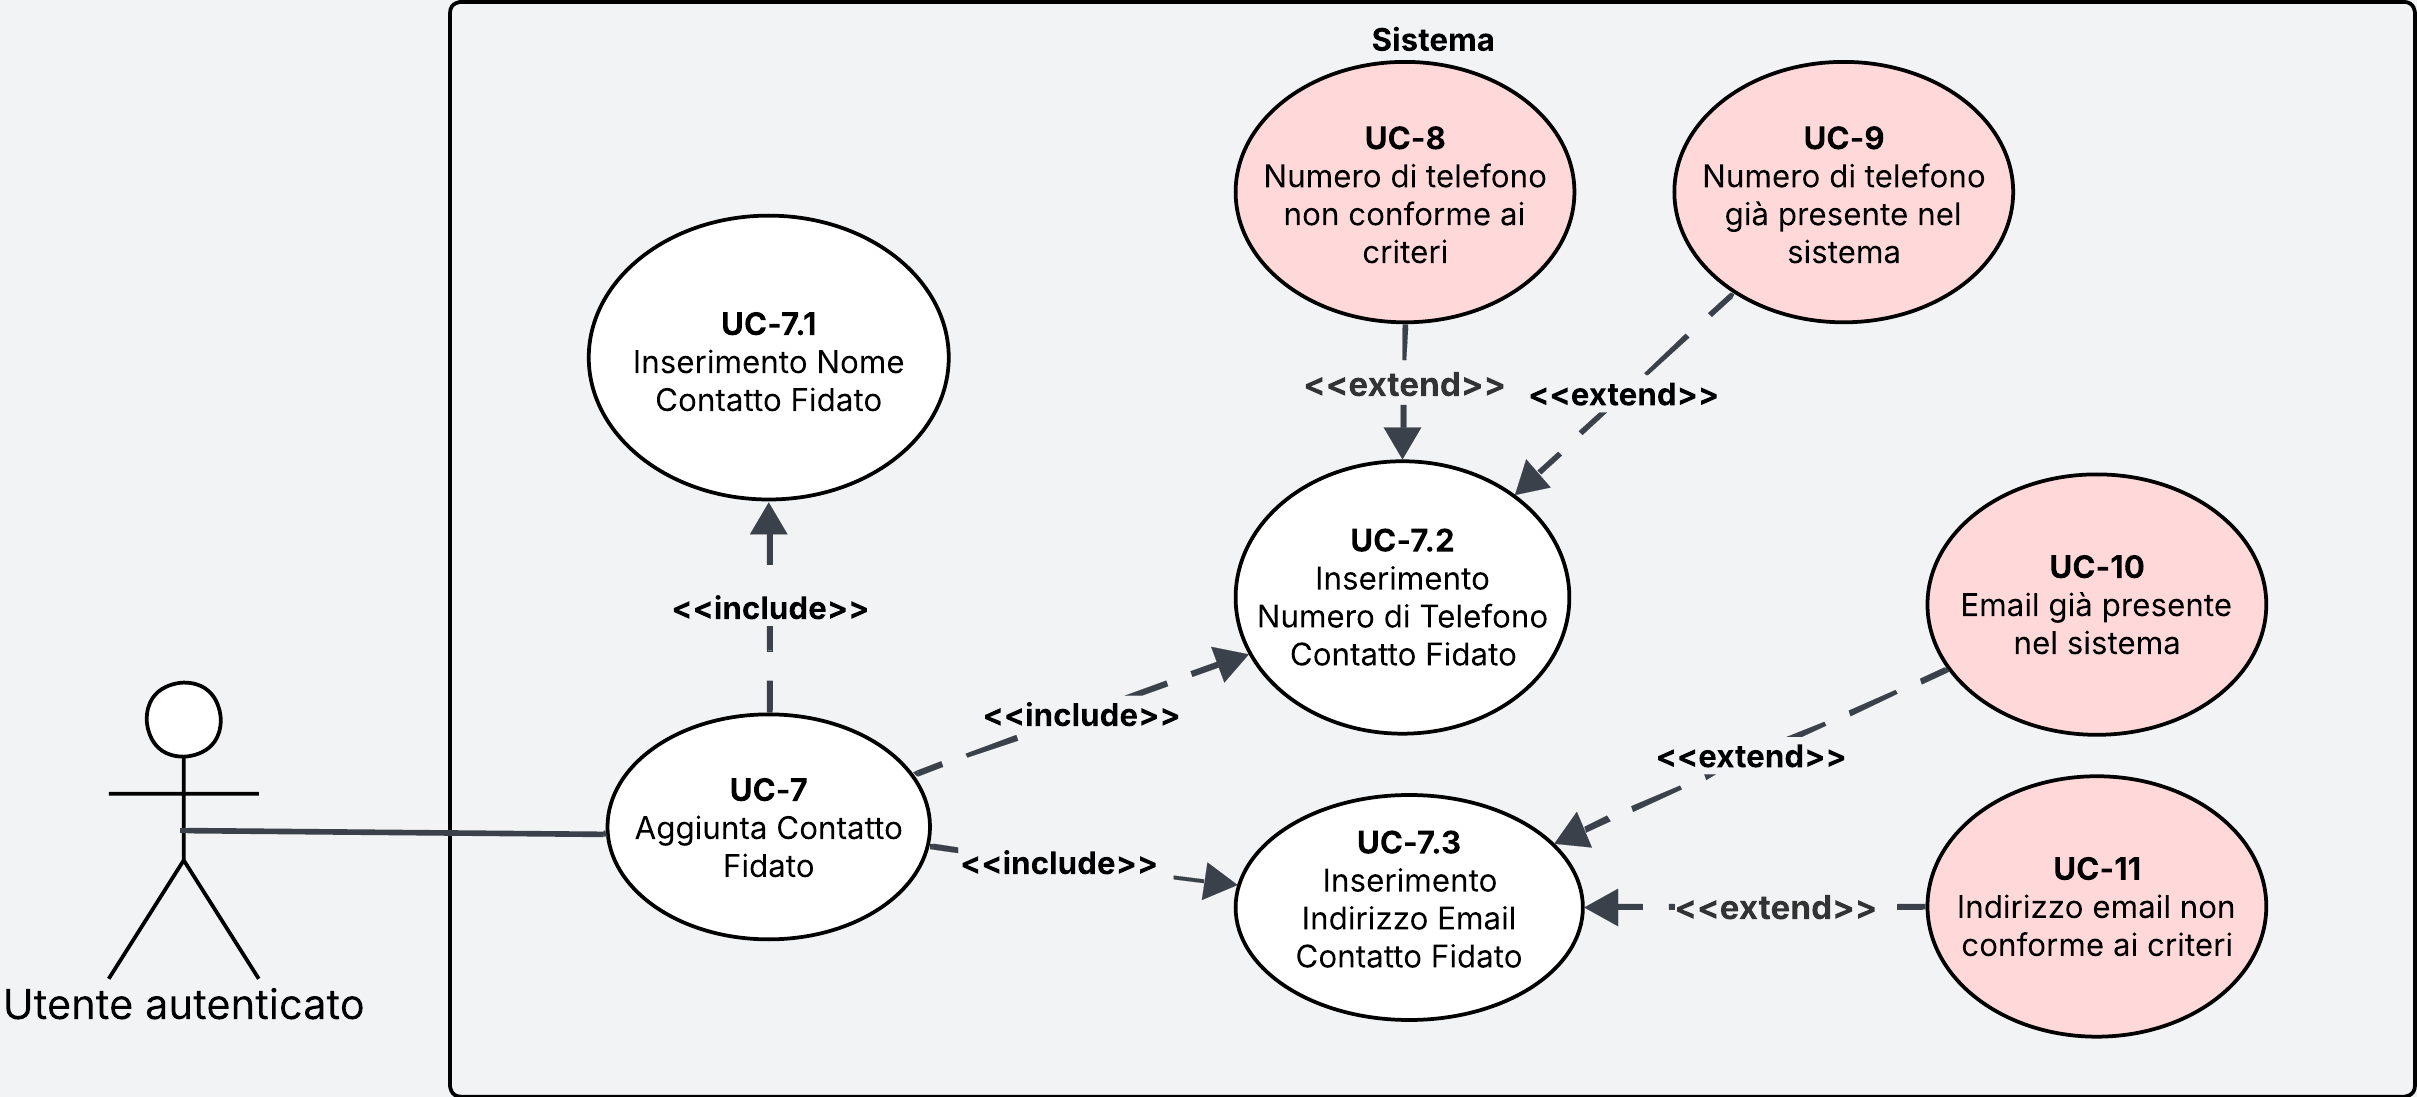
\includegraphics[width=1\textwidth]{use_case/UC-7-aggiunta-contatto-fidato.png}
    \caption{Diagramma del caso d'uso UC-7 con relativi sottocasi d'uso}
    \label{fig:UC-7}
\end{figure}
\begin{itemize}
    \item \textbf{Attore principale:} \term{Utente} Autenticato
    \item \textbf{Pre-condizioni:} 
    \begin{itemize}
        \item Il sistema è attivo
        \item L'attore ha selezionato la voce per l'aggiunta di un nuovo contatto fidato
    \end{itemize}
    \item \textbf{Post-condizioni:}
    \begin{itemize}
        \item Le informazioni del contatto fidato sono memorizzate nel sistema
    \end{itemize}
    \item \textbf{Scenario principale:} 
    \begin{itemize}
        \item L'attore seleziona la voce per l'aggiunta del contatto fidato
        \item L'attore inserisce il nome del contatto fidato $\rightarrow$ \hyperref[subsec:UC-7.1]{UC-7.1}
        \item L'attore inserisce il numero di telefono del contatto fidato $\rightarrow$ \hyperref[subsec:UC-7.2]{UC-7.2}
        \item L'attore inserisce l'indirizzo email del contatto fidato $\rightarrow$ \hyperref[subsec:UC-7.3]{UC-7.3}
        \item L'attore seleziona la voce per il salvataggio del contatto fidato nella rete di contatti
    \end{itemize}
    \item \textbf{Inclusioni:}
    \begin{itemize}
        \item \hyperref[subsec:UC-7.1]{UC-7.1}
        \item \hyperref[subsec:UC-7.2]{UC-7.2}
        \item \hyperref[subsec:UC-7.3]{UC-7.3}
    \end{itemize}
    \item \textbf{Trigger:} L'attore vuole aggiungere un nuovo contatto fidato nella propria rete
\end{itemize}

\subsubsection{UC-7.1 - Inserimento nome contatto fidato} \label{subsec:UC-7.1}
\begin{itemize}
    \item \textbf{Attore principale:} \term{Utente} Generico
    \item \textbf{Pre-condizioni:}
    \begin{itemize}
        \item Il sistema è attivo
        \item L'attore ha selezionato la voce per l'aggiunta di un nuovo contatto fidato
    \end{itemize}
    \item \textbf{Post-condizioni:} 
    \begin{itemize}
        \item Il sistema riceve il nome del contatto fidato che l'attore vuole inserire
    \end{itemize}
    \item \textbf{Scenario principale:} 
    \begin{itemize}
        \item L'attore inserisce il nome del contatto fidato da memorizzare
    \end{itemize}
    \item \textbf{Trigger:} L'attore vuole inserire un nuovo contatto nella propria rete di contatti fidati
\end{itemize}

\subsubsection{UC-7.2 - Inserimento numero di telefono contatto fidato} \label{subsec:UC-7.2}
\begin{itemize}
    \item \textbf{Attore principale:} \term{Utente} Generico
    \item \textbf{Pre-condizioni:}
    \begin{itemize}
        \item Il sistema è attivo
        \item L'attore ha selezionato la voce per l'aggiunta di un nuovo contatto fidato
    \end{itemize}
    \item \textbf{Post-condizioni:} 
    \begin{itemize}
        \item Il sistema riceve il numero di telefono del contatto fidato che l'attore vuole inserire
    \end{itemize}
    \item \textbf{Scenario principale:} 
    \begin{itemize}
        \item L'attore inserisce il numero di telefono del contatto fidato da memorizzare
    \end{itemize}
    \item \textbf{Scenario secondario:}
    \begin{itemize}
        \item Il numero inserito dall'attore non è conforme ai criteri dell'applicazione $\rightarrow$ \hyperref[subsec:UC-8]{UC-8}
        \item Il numero inserito è già presente nel sistema $\rightarrow$ \hyperref[subsec:UC-9]{UC-9}
    \end{itemize}
    \item \textbf{Estensioni:} 
    \begin{itemize}
        \item \hyperref[subsec:UC-8]{UC-8}
        \item \hyperref[subsec:UC-9]{UC-9}
    \end{itemize}
    \item \textbf{Trigger:} L'attore vuole inserire un nuovo contatto nella propria rete di contatti fidati
\end{itemize}

\subsubsection{UC-7.3 - Inserimento indirizzo email contatto fidato} \label{subsec:UC-7.3}
\begin{itemize}
    \item \textbf{Attore principale:} \term{Utente} Generico
    \item \textbf{Pre-condizioni:}
    \begin{itemize}
        \item Il sistema è attivo
        \item L'attore ha selezionato la voce per l'aggiunta di un nuovo contatto fidato
    \end{itemize}
    \item \textbf{Post-condizioni:} 
    \begin{itemize}
        \item Il sistema riceve l'indirizzo email del contatto fidato che l'attore vuole inserire
    \end{itemize}
    \item \textbf{Scenario principale:} 
    \begin{itemize}
        \item L'attore inserisce l'indirizzo email del contatto fidato da memorizzare
    \end{itemize}
    \item \textbf{Scenario secondario:}
    \begin{itemize}
        \item L'indirizzo email inserito dall'attore non è conforme ai criteri dell'applicazione $\rightarrow$ \hyperref[subsec:UC-11]{UC-11}
        \item L'indirizzo email inserito è già presente nel sistema $\rightarrow$ \hyperref[subsec:UC-10]{UC-10}
    \end{itemize}
    \item \textbf{Estensioni:} 
    \begin{itemize}
        \item \hyperref[subsec:UC-11]{UC-11}
        \item \hyperref[subsec:UC-10]{UC-10}
    \end{itemize}
    \item \textbf{Trigger:} L'attore vuole inserire un nuovo contatto nella propria rete di contatti fidati
\end{itemize}

\subsubsection{UC-8 Numero di telefono non conforme ai criteri} \label{subsec:UC-8}
\begin{itemize}
    \item \textbf{Attore principale:} \term{Utente} Generico
    \item \textbf{Pre-condizioni:}
    \begin{itemize}
        \item Il sistema è attivo
        \item L'attore ha selezionato la voce per l'aggiunta di un nuovo contatto fidato
        \item L'attore ha inserito un numero di telefono non conforme ai criteri dell'applicazione
    \end{itemize}
    \item \textbf{Post-condizioni:} 
    \begin{itemize}
        \item Il sistema notifica all'attore che il numero di telefono inserito non è valido
        \item L'attore può correggere il numero di telefono inserito
    \end{itemize}
    \item \textbf{Scenario principale:} 
    \begin{itemize}        
        \item L'attore inserisce un numero di telefono non conforme ai criteri dell'applicazione
        \item Il sistema \ignoreglossary{verifica} il numero di telefono e rileva che non è valido
        \item Il sistema notifica all'attore l'errore e richiede la correzione del numero di telefono
    \end{itemize}
    \item \textbf{Trigger:} L'attore ha inserito un numero di telefono non conforme ai criteri dell'applicazione
\end{itemize}

\subsubsection{UC-9 - Numero di telefono già presente nel sistema} \label{subsec:UC-9}
\begin{itemize}
    \item \textbf{Attore principale:} \term{Utente} Autenticato
    \item \textbf{Pre-condizioni:}
    \begin{itemize}
        \item Il sistema è attivo
        \item L'attore sta aggiungendo o modificando un contatto fidato
        \item L'attore ha inserito un numero di telefono già associato a un altro contatto
    \end{itemize}
    \item \textbf{Post-condizioni:}
    \begin{itemize}
        \item Il sistema notifica la presenza del duplicato
        \item Il salvataggio del contatto viene bloccato
    \end{itemize}
    \item \textbf{Scenario principale:}
    \begin{itemize}
        \item Il sistema rileva che il numero di telefono inserito è già presente in rubrica
        \item Il sistema mostra un messaggio di errore specifico per il numero duplicato
        \item Il sistema richiede all'attore di inserire un numero diverso
    \end{itemize}
    \item \textbf{Trigger:} Rilevamento di un numero di telefono duplicato durante il salvataggio o l'inserimento
\end{itemize}

\subsubsection{UC-10 - Email già presente nel sistema} \label{subsec:UC-10}
\begin{itemize}
    \item \textbf{Attore principale:} \term{Utente} Autenticato
    \item \textbf{Pre-condizioni:}
    \begin{itemize}
        \item Il sistema è attivo
        \item L'attore sta aggiungendo o modificando un contatto fidato
        \item L'attore ha inserito un indirizzo email già associato a un altro contatto
    \end{itemize}
    \item \textbf{Post-condizioni:}
    \begin{itemize}
        \item Il sistema notifica la presenza del duplicato
        \item Il salvataggio del contatto viene bloccato
    \end{itemize}
    \item \textbf{Scenario principale:}
    \begin{itemize}
        \item Il sistema rileva che l'email inserita è già presente in rubrica
        \item Il sistema mostra un messaggio di errore specifico per l'email duplicata
        \item Il sistema richiede all'attore di inserire un'email diversa
    \end{itemize}
    \item \textbf{Trigger:} Rilevamento di un'email duplicata durante il salvataggio o l'inserimento
\end{itemize}

\subsubsection{UC-11 Indirizzo email non conforme ai criteri} \label{subsec:UC-11}
\begin{itemize}
    \item \textbf{Attore principale:} \term{Utente} Generico
    \item \textbf{Pre-condizioni:}
    \begin{itemize}
        \item Il sistema è attivo
        \item L'attore ha selezionato la voce per l'aggiunta di un nuovo contatto fidato
        \item L'attore ha inserito un indirizzo email non conforme ai criteri dell'applicazione
    \end{itemize}
    \item \textbf{Post-condizioni:} 
    \begin{itemize}
        \item Il sistema notifica all'attore che l'indirizzo email inserito non è valido
        \item L'attore può correggere l'indirizzo email inserito
    \end{itemize}
    \item \textbf{Scenario principale:} 
    \begin{itemize}        
        \item L'attore inserisce un indirizzo email non conforme ai criteri dell'applicazione
        \item Il sistema \ignoreglossary{verifica} l'indirizzo email e rileva che non è valido
        \item Il sistema notifica all'attore l'errore e richiede la correzione dell'indirizzo email
    \end{itemize}
    \item \textbf{Trigger:} L'attore ha inserito un indirizzo email non conforme ai criteri dell'applicazione
\end{itemize}

% ===== UC-12: MODIFICA CONTATTO FIDATO =====

\subsubsection{UC-12 - Modifica contatto fidato} \label{subsec:UC-12}
\begin{tcolorbox}[colback=gray!10,colframe=gray!50,title=Nota]
{\small Il caso d'uso \hyperref[subsec:UC-12]{UC-12} è suddiviso nei casi d'uso inclusi \hyperref[subsec:UC-12.1]{UC-12.1}, \hyperref[subsec:UC-12.2]{UC-12.2} e \hyperref[subsec:UC-12.3]{UC-12.3}, che ne dettagliano il comportamento.
Il diagramma riportato di seguito mostra anche ulteriori casi d'uso correlati (\hyperref[subsec:UC-8]{UC-8}, \hyperref[subsec:UC-9]{UC-9}, \hyperref[subsec:UC-10]{UC-10} e \hyperref[subsec:UC-11]{UC-11}), la cui descrizione dettagliata è riportata nelle sezioni precedenti del documento.}
\end{tcolorbox}
\begin{figure}[H]
    \centering
    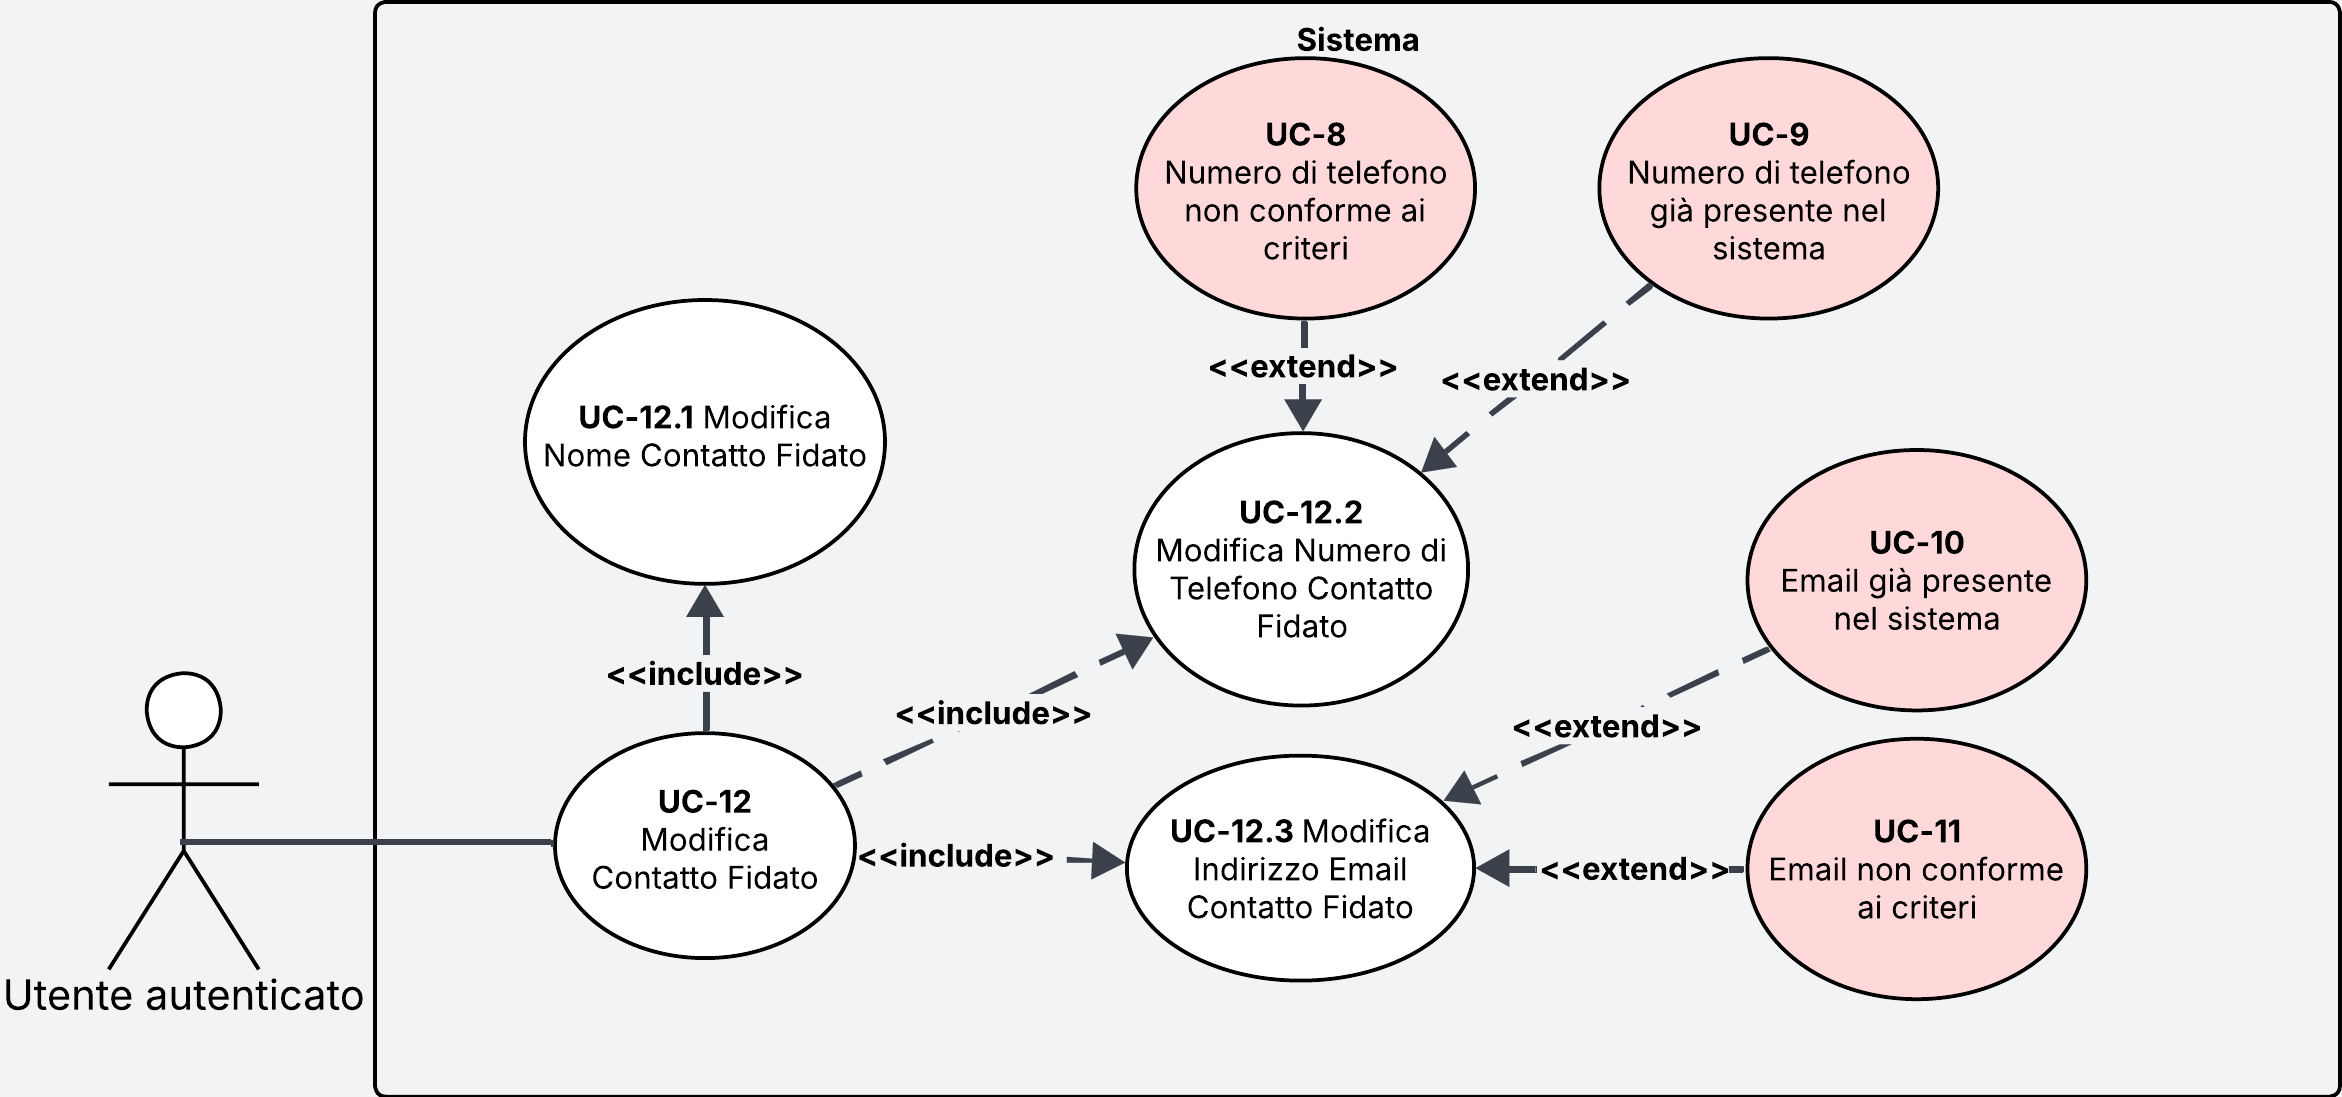
\includegraphics[width=1\textwidth]{use_case/UC-12-modifica-contatto-fidato.png}
    \caption{Diagramma del caso d'uso UC-12}
    \label{fig:UC-12}
\end{figure}
\begin{itemize}
    \item \textbf{Attore principale:} \term{Utente} Autenticato
    \item \textbf{Pre-condizioni:} 
    \begin{itemize}
        \item Il sistema è attivo
        \item Almeno un contatto fidato è presente nella rete dei contatti
        \item L'attore ha selezionato la voce per la modifica di un contatto fidato
    \end{itemize}
    \item \textbf{Post-condizioni:}
    \begin{itemize}
        \item Le nuove informazioni del contatto fidato sono memorizzate nel sistema
    \end{itemize}
    \item \textbf{Scenario principale:} 
    \begin{itemize}
        \item L'attore seleziona la voce per la modifica del contatto fidato
        \item L'attore modifica il nome del contatto fidato $\rightarrow$ \hyperref[subsec:UC-12.1]{UC-12.1}
        \item L'attore modifica il numero di telefono del contatto fidato $\rightarrow$ \hyperref[subsec:UC-12.2]{UC-12.2}
        \item L'attore modifica l'indirizzo email del contatto fidato $\rightarrow$ \hyperref[subsec:UC-12.3]{UC-12.3}
        \item L'attore seleziona la voce per il salvataggio delle modifiche del contatto fidato nella rete di contatti
    \end{itemize}
    \item \textbf{Inclusioni:}
    \begin{itemize}
        \item \hyperref[subsec:UC-12.1]{UC-12.1}
        \item \hyperref[subsec:UC-12.2]{UC-12.2}
        \item \hyperref[subsec:UC-12.3]{UC-12.3}
    \end{itemize}
    \item \textbf{Trigger:} L'attore vuole modificare un contatto fidato nella propria rete
\end{itemize}

\subsubsection{UC-12.1 - Modifica nome contatto fidato} \label{subsec:UC-12.1}
\begin{itemize}
    \item \textbf{Attore principale:} \term{Utente} Autenticato
    \item \textbf{Pre-condizioni:}
    \begin{itemize}
        \item Il sistema è attivo
        \item L'attore ha selezionato la voce per la modifica di un contatto fidato
        \item L'attore ha selezionato il campo del nome del contatto fidato da modificare
    \end{itemize}
    \item \textbf{Post-condizioni:} 
    \begin{itemize}
        \item Il sistema riceve il nome del contatto fidato che l'attore vuole modificare
    \end{itemize}
    \item \textbf{Scenario principale:} 
    \begin{itemize}
        \item L'attore inserisce il nuovo nome del contatto fidato da memorizzare
        \item L'attore salva le modifiche apportate
    \end{itemize}
    \item \textbf{Trigger:} L'attore vuole modificare il nome di un contatto fidato presente nella propria rete di contatti fidati
\end{itemize}

\subsubsection{UC-12.2 - Modifica numero di telefono contatto fidato} \label{subsec:UC-12.2}
\begin{itemize}
    \item \textbf{Attore principale:} \term{Utente} Autenticato
    \item \textbf{Pre-condizioni:}
    \begin{itemize}
        \item Il sistema è attivo
        \item L'attore ha selezionato la voce per la modifica di un contatto fidato
        \item L'attore ha selezionato il campo del numero di telefono del contatto fidato da modificare
    \end{itemize}
    \item \textbf{Post-condizioni:} 
    \begin{itemize}
        \item Il sistema riceve il numero di telefono del contatto fidato che l'attore vuole modificare
    \end{itemize}
    \item \textbf{Scenario principale:} 
    \begin{itemize}
        \item L'attore inserisce il numero di telefono del contatto fidato da memorizzare
        \item L'attore salva le modifiche apportate
    \end{itemize}
    \item \textbf{Scenario secondario:}
    \begin{itemize}
        \item Il numero inserito dall'attore non è conforme ai criteri dell'applicazione $\rightarrow$ \hyperref[subsec:UC-8]{UC-8}
        \item Il numero modificato è già presente nel sistema per un altro contatto $\rightarrow$ \hyperref[subsec:UC-9]{UC-9}
    \end{itemize}
    \item \textbf{Estensioni:}
    \begin{itemize}
        \item \hyperref[subsec:UC-8]{UC-8}
        \item \hyperref[subsec:UC-9]{UC-9}
    \end{itemize}
    \item \textbf{Trigger:} L'attore vuole modificare il numero di telefono di un contatto fidato presente nella propria rete di contatti fidati
\end{itemize}

\subsubsection{UC-12.3 - Modifica indirizzo email contatto fidato} \label{subsec:UC-12.3}
\begin{itemize}
    \item \textbf{Attore principale:} \term{Utente} Autenticato
    \item \textbf{Pre-condizioni:}
    \begin{itemize}
        \item Il sistema è attivo
        \item L'attore ha selezionato la voce per la modifica di un contatto fidato
        \item L'attore ha selezionato il campo dell'indirizzo email del contatto fidato da modificare
    \end{itemize}
    \item \textbf{Post-condizioni:} 
    \begin{itemize}
        \item Il sistema riceve l'indirizzo email del contatto fidato che l'attore vuole modificare
    \end{itemize}
    \item \textbf{Scenario principale:} 
    \begin{itemize}
        \item L'attore inserisce l'indirizzo email del contatto fidato da memorizzare
        \item L'attore salva le modifiche apportate
    \end{itemize}
    \item \textbf{Scenario secondario:}
    \begin{itemize}
        \item L'indirizzo email inserito dall'attore non è conforme ai criteri dell'applicazione $\rightarrow$ \hyperref[subsec:UC-11]{UC-11}
        \item L'indirizzo email modificato è già presente nel sistema per un altro contatto $\rightarrow$ \hyperref[subsec:UC-10]{UC-10}
    \end{itemize}
    \item \textbf{Estensioni:}
    \begin{itemize}
        \item \hyperref[subsec:UC-11]{UC-11}
        \item \hyperref[subsec:UC-10]{UC-10}
    \end{itemize}
    \item \textbf{Trigger:} L'attore vuole modificare l'indirizzo email di un contatto fidato presente nella propria rete di contatti fidati
\end{itemize}

% ===== UC-13 - CANCELLAZIONE CONTATTO FIDATO =====

\subsubsection{UC-13 Eliminazione contatto fidato} \label{subsec:UC-13}
\begin{figure}[H]
    \centering
    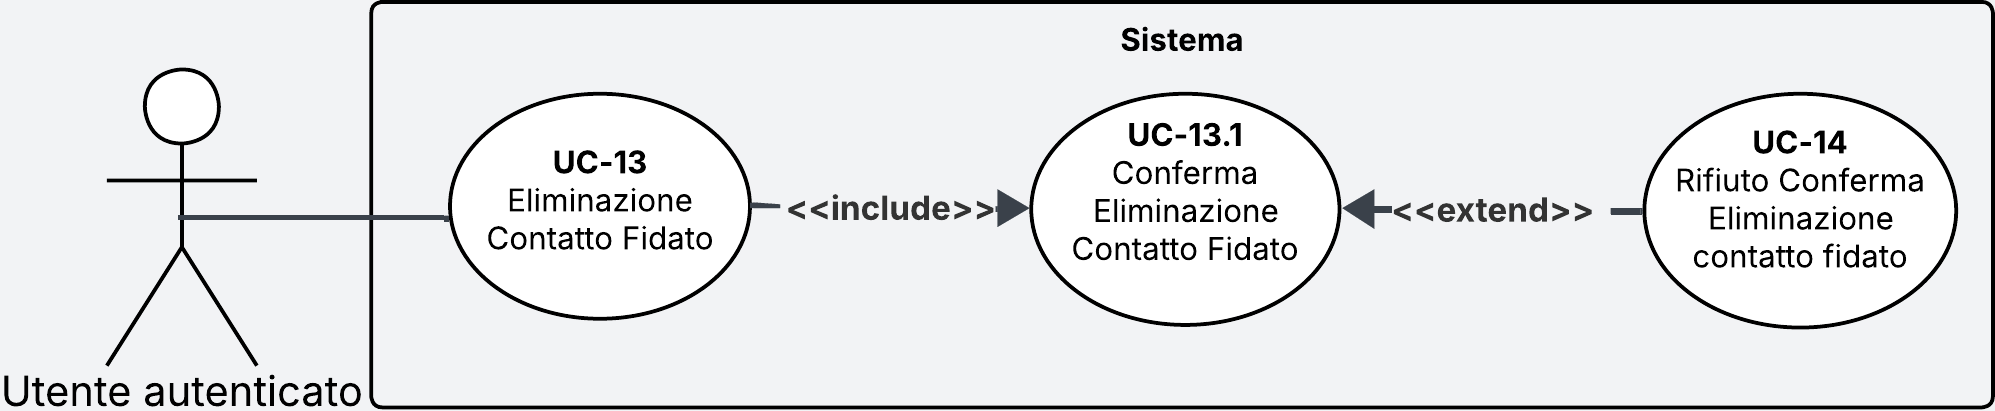
\includegraphics[width=1\textwidth]{use_case/UC-13-impostazioni.png}
    \caption{Diagramma del caso d'uso UC-13}
    \label{fig:UC-13}
\end{figure}
\begin{itemize}
    \item \textbf{Attore principale:} \term{Utente} Autenticato
    \item \textbf{Pre-condizioni:}
    \begin{itemize}
        \item Il sistema è attivo
        \item L'attore sta visualizzando le informazioni di un contatto fidato
        \item Almeno un contatto fidato è presente nella rete dei contatti fidati
    \end{itemize}
    \item \textbf{Post-condizioni:}
    \begin{itemize}
        \item Il sistema rimuove un contatto fidato dalla rete dei contatti fidati dell'attore
    \end{itemize}
    \item \textbf{Scenario principale:} 
    \begin{itemize}
        \item L'attore seleziona un contatto dalla lista dei contatti fidati
        \item L'attore seleziona la voce di cancellazione per quel contatto fidato
        \item L'attore conferma l'eliminazione del contatto fidato $\rightarrow$ \hyperref[subsec:UC-13.1]{UC-13.1}
        \item Il sistema rimuove il contatto fidato scelto dall'attore dalla rete dei contatti fidati dell'attore
    \end{itemize}
    \item \textbf{Inclusioni:} 
    \begin{itemize}
        \item \hyperref[subsec:UC-13.1]{UC-13.1}
    \end{itemize}
    \item \textbf{Trigger:} L'attore vuole rimuovere un contatto dalla propria rete di contatti fidati
\end{itemize}

\subsubsection{UC-13.1 Conferma eliminazione contatto fidato} \label{subsec:UC-13.1}
\begin{itemize}
    \item \textbf{Attore principale:} \term{Utente} Autenticato
    \item \textbf{Pre-condizioni:}
    \begin{itemize}
        \item Il sistema è attivo
        \item L'attore ha selezionato la voce di cancellazione per quel contatto fidato
    \end{itemize}
    \item \textbf{Post-condizioni:}
    \begin{itemize}
        \item Il sistema riceve la conferma dell'attore di rimuovere un contatto fidato dalla propria rete dei contatti fidati
    \end{itemize}
    \item \textbf{Scenario principale:}
    \begin{itemize}
        \item L'attore conferma l'eliminazione del contatto fidato
        \item Il sistema rimuove il contatto fidato scelto dall'attore dalla rete dei contatti fidati dell'attore
    \end{itemize}
    \item \textbf{Trigger:} L'attore ha scelto la voce di cancellazione per quel contatto fidato
\end{itemize}

% ==== DEAD MAN'S SWITCH ====

\subsubsection{UC-15 - Impostazione timer prima inattività} \label{sec:UC-15}
\begin{figure}[H]
    \centering
    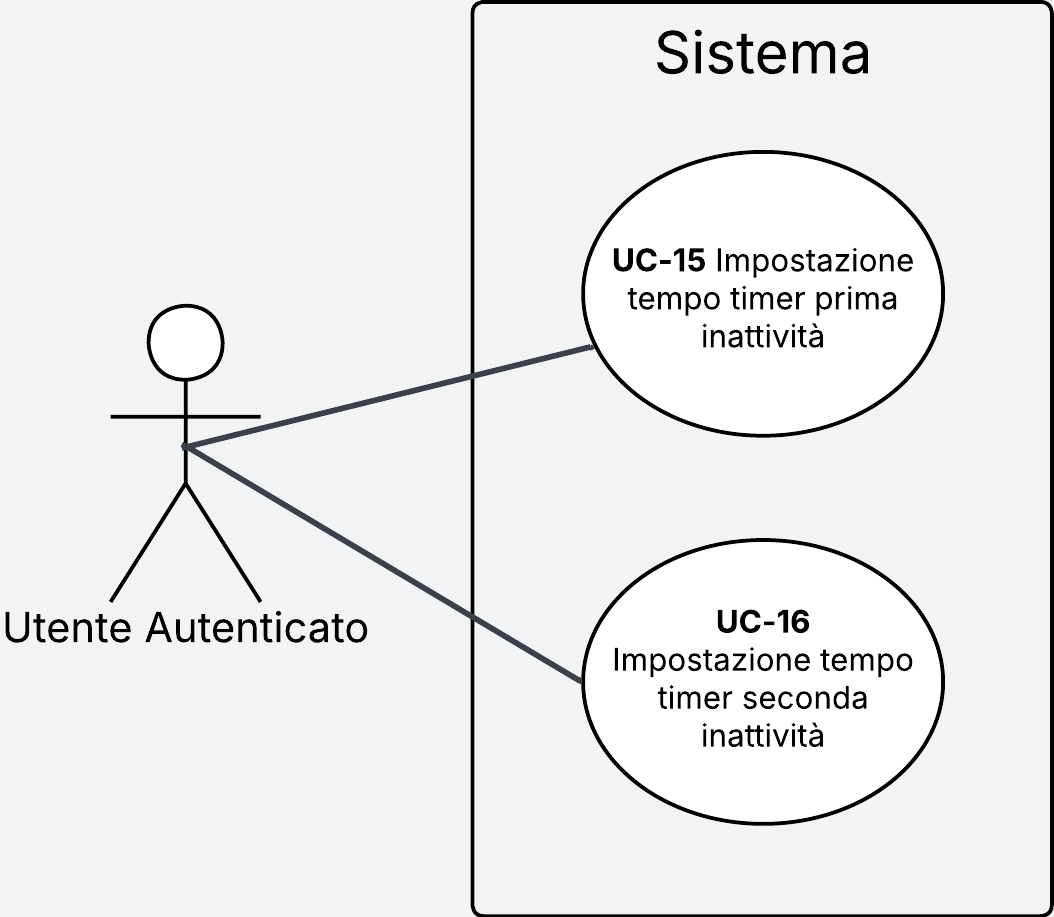
\includegraphics[width=1\textwidth]{use_case/UC-15-16-dmswitch.png}
    \caption{Diagramma dei casi d'uso UC-15 e UC-16}
    \label{fig:UC-15}
\end{figure}
\begin{itemize}
    \item \textbf{Attore principale:} \term{Utente} Autenticato
    \item \textbf{Pre-condizioni:}
    \begin{itemize}
        \item Il sistema è attivo
        \item La funzionalità Dead Man's Switch è abilitata
        \item L'attore ha effettuato l'accesso alle impostazioni del Dead Man's Switch
    \end{itemize}
    \item \textbf{Post-condizioni:}
    \begin{itemize}
        \item Il sistema memorizza l'intervallo di tempo per il primo controllo di inattività
    \end{itemize}
    \item \textbf{Scenario principale:} 
    \begin{itemize}
        \item L'attore seleziona la voce per l'impostazione del primo timer
        \item L'attore imposta la durata desiderata dopo la quale il sistema invierà la mail di controllo all'attore
        \item L'attore conferma la scelta
        \item Il sistema aggiorna la configurazione
    \end{itemize}
    \item \textbf{Trigger:} L'attore vuole definire dopo quanto tempo il sistema deve verificare la sua presenza
\end{itemize}

\subsubsection{UC-16 - Impostazione timer seconda inattività} \label{sec:UC-16}
\begin{itemize}
    \item \textbf{Attore principale:} \term{Utente} Autenticato
    \item \textbf{Pre-condizioni:}
    \begin{itemize}
        \item Il sistema è attivo
        \item La funzionalità Dead Man's Switch è abilitata
        \item L'attore si trova nelle impostazioni del Dead Man's Switch
        \item Il timer di prima inattività è stato configurato
    \end{itemize}
    \item \textbf{Post-condizioni:}
    \begin{itemize}
        \item Il sistema memorizza l'intervallo di tempo per il secondo controllo di inattività
    \end{itemize}
    \item \textbf{Scenario principale:}
    \begin{itemize}
        \item L'attore seleziona la voce per l'impostazione del secondo timer
        \item L'attore imposta la durata che deve trascorrere tra la mail di controllo e l'invio del messaggio di SOS ai contatti fidati
        \item L'attore conferma la scelta
        \item Il sistema aggiorna la configurazione
    \end{itemize}
    \item \textbf{Trigger:} L'attore vuole definire quanto tempo ha per rispondere alla mail di controllo prima che parta l'allarme
\end{itemize}

\subsubsection{UC-17 - Modifica mail di avviso} \label{sec:UC-17}
\begin{figure}[H]
    \centering
    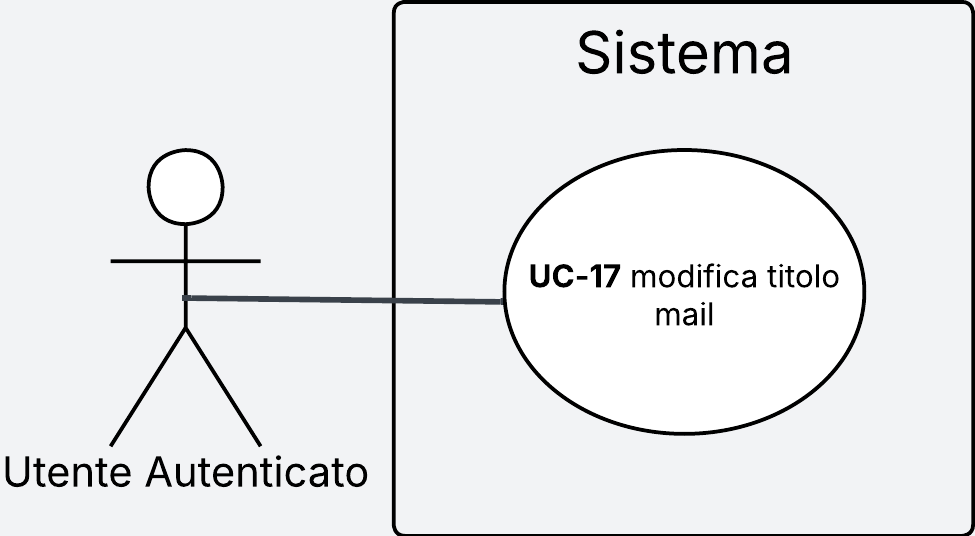
\includegraphics[width=1\textwidth]{use_case/UC-17-dmswitch.png}
    \caption{Diagramma del caso d'uso UC-17}
    \label{fig:UC-17}
\end{figure}
\begin{itemize}
    \item \textbf{Attore principale:} \term{Utente} Autenticato
    \item \textbf{Pre-condizioni:}
    \begin{itemize}
        \item Il sistema è attivo
        \item La funzionalità Dead Man's Switch è abilitata
        \item L'attore ha selezionato l'opzione di modifica della mail di avviso
    \end{itemize}
    \item \textbf{Post-condizioni:}
    \begin{itemize}
        \item Le preferenze dell'attore sono salvate nel sistema
    \end{itemize}
    \item \textbf{Scenario principale:} 
    \begin{itemize}
        \item L'attore modifica il titolo della mail \hyperref[sec:UC-17.1]{UC-17.1}
        \item L'attore modifica il corpo della mail \hyperref[sec:UC-17.2]{UC-17.2}
        \item L'attore seleziona la voce di salvataggio delle modifiche per la mail di avviso
    \end{itemize}
    \item \textbf{Inclusioni:}
    \begin{itemize}
        \item \hyperref[sec:UC-17.1]{UC-17.1}
        \item \hyperref[sec:UC-17.2]{UC-17.2}
    \end{itemize}
    \item \textbf{Trigger:} L'attore vuole personalizzare la mail di avviso che riceverà in caso di inutilizzo prolungato dell'applicazione
\end{itemize}

\subsubsection{UC-17.1 - Modifica titolo mail di avviso} \label{sec:UC-17.1}
\begin{itemize}
    \item \textbf{Attore principale:} \term{Utente} Autenticato
    \item \textbf{Pre-condizioni:}
    \begin{itemize}
        \item Il sistema è attivo
        \item La funzionalità Dead Man's Switch è abilitata
        \item L'attore ha selezionato il campo per la modifica del titolo della mail di avviso
    \end{itemize}
    \item \textbf{Post-condizioni:}
    \begin{itemize}
        \item La modifica del titolo della mail di avviso viene salvata dal sistema
    \end{itemize}
    \item \textbf{Scenario principale:} 
    \begin{itemize}
        \item L'attore inserisce il titolo della mail di avviso
    \end{itemize}
    \item \textbf{Trigger:} L'attore vuole personalizzare il titolo della mail di avviso che riceverà in caso di inutilizzo prolungato dell'applicazione
\end{itemize}

\subsubsection{UC-17.2 - Modifica corpo mail di avviso} \label{sec:UC-17.2}
\begin{itemize}
    \item \textbf{Attore principale:} \term{Utente} Autenticato
    \item \textbf{Pre-condizioni:}
    \begin{itemize}
        \item Il sistema è attivo
        \item La funzionalità Dead Man's Switch è abilitata
        \item L'attore ha selezionato l'opzione di modifica della mail di avviso
        \item L'attore ha selezionato il campo per la modifica del corpo della mail di avviso
    \end{itemize}
    \item \textbf{Post-condizioni:}
    \begin{itemize}
        \item La modifica del corpo della mail di avviso viene salvata dal sistema
    \end{itemize}
    \item \textbf{Scenario principale:} 
    \begin{itemize}
        \item L'attore inserisce il corpo della mail di avviso
    \end{itemize}
    \item \textbf{Trigger:} L'attore vuole personalizzare il corpo della mail che riceverà in caso di inutilizzo prolungato dell'applicazione
\end{itemize}

\subsubsection{UC-18 - Visualizzazione preview mail di avviso} \label{sec:UC-18}
\begin{figure}[H]
    \centering
    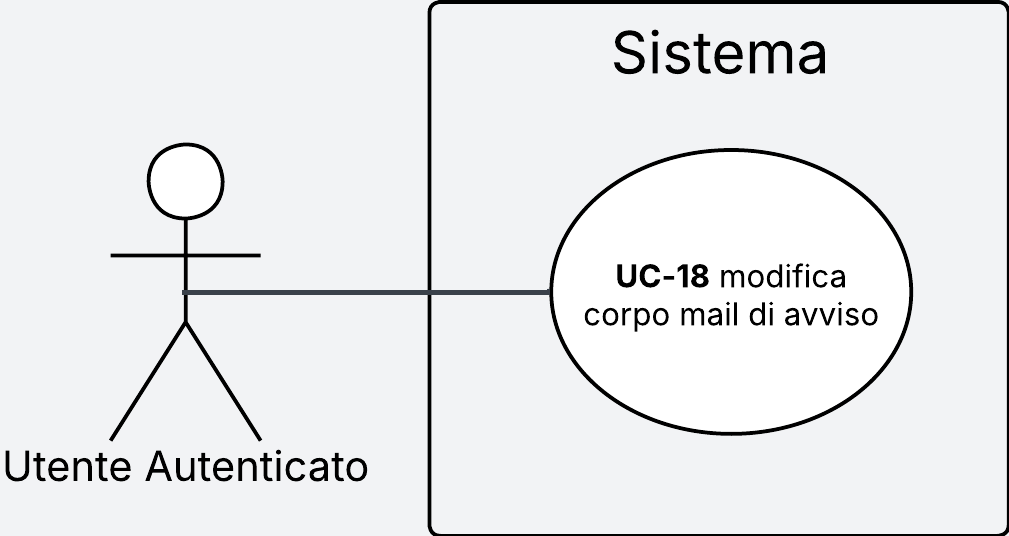
\includegraphics[width=1\textwidth]{use_case/UC-18-dmswitch.png}
    \caption{Diagramma del caso d'uso UC-18}
    \label{fig:UC-18}
\end{figure}
\begin{itemize}
    \item \textbf{Attore principale:} \term{Utente} Autenticato
    \item \textbf{Pre-condizioni:}
    \begin{itemize}
        \item Il sistema è attivo
        \item La funzionalità Dead Man's Switch è abilitata
        \item L'attore vuole verificare l'aspetto della mail configurata
    \end{itemize}
    \item \textbf{Post-condizioni:}
    \begin{itemize}
        \item L'attore visualizza una preview fedele della mail che verrà inviata
    \end{itemize}
    \item \textbf{Scenario principale:} 
    \begin{itemize}
        \item Il sistema recupera le preferenze di formattazione della mail di avviso
        \item Il sistema compone la preview del messaggio
        \item Il sistema visualizza il titolo della mail $\rightarrow$ \hyperref[subsec:UC-18.1]{UC-18.1}
        \item Il sistema visualizza il corpo della mail $\rightarrow$ \hyperref[subsec:UC-18.2]{UC-18.2}
    \end{itemize}
    \item \textbf{Scenario secondario:} 
    \begin{itemize}
        \item Errore nel recupero della configurazione 
    \end{itemize}
    \item \textbf{Inclusioni:}
    \begin{itemize}
        \item \hyperref[subsec:UC-18.1]{UC-18.1}
        \item \hyperref[subsec:UC-18.2]{UC-18.2}
    \end{itemize}
    \item \textbf{Trigger:} L'attore vuole visualizzare le informazioni della mail che riceverà in caso di inutilizzo prolungato dell'applicazione
\end{itemize}

\subsubsection{UC-18.1 - Visualizzazione corpo della mail di avviso} \label{subsec:UC-18.1}
\begin{itemize}
    \item \textbf{Attore principale:} \term{Utente} Autenticato
    \item \textbf{Pre-condizioni:}
    \begin{itemize}
        \item La funzionalità Dead Man's Switch è abilitata
        \item Il sistema sta renderizzando la preview
    \end{itemize}
    \item \textbf{Post-condizioni:} Il contenuto principale della mail è visibile
    \item \textbf{Scenario principale:} 
    \begin{itemize}
        \item Il sistema mostra il testo del messaggio nel corpo della preview
    \end{itemize}
    \item \textbf{Trigger:} L'attore vuole visualizzare la preview della mail che riceverà in caso di inutilizzo prolungato dell'applicazione
\end{itemize}

\subsubsection{UC-18.2 - Visualizzazione titolo mail di avviso} \label{subsec:UC-18.2}
\begin{itemize}
    \item \textbf{Attore principale:} \term{Utente} Autenticato
    \item \textbf{Pre-condizioni:}
    \begin{itemize}
        \item La funzionalità Dead Man's Switch è abilitata
        \item Il sistema sta visualizzando la preview
    \end{itemize}
    \item \textbf{Post-condizioni:} L'oggetto della mail è visibile
    \item \textbf{Scenario principale:} 
    \begin{itemize}
        \item Il sistema mostra il testo configurato come oggetto della mail nell'header della preview
    \end{itemize}
    \item \textbf{Trigger:} L'attore vuole visualizzare il titolo della mail che riceverà in caso di inutilizzo prolungato dell'applicazione
\end{itemize}

\subsubsection{UC-19 - Attivazione Dead Man's Switch} \label{sec:UC-19}
\begin{figure}[H]
    \centering
    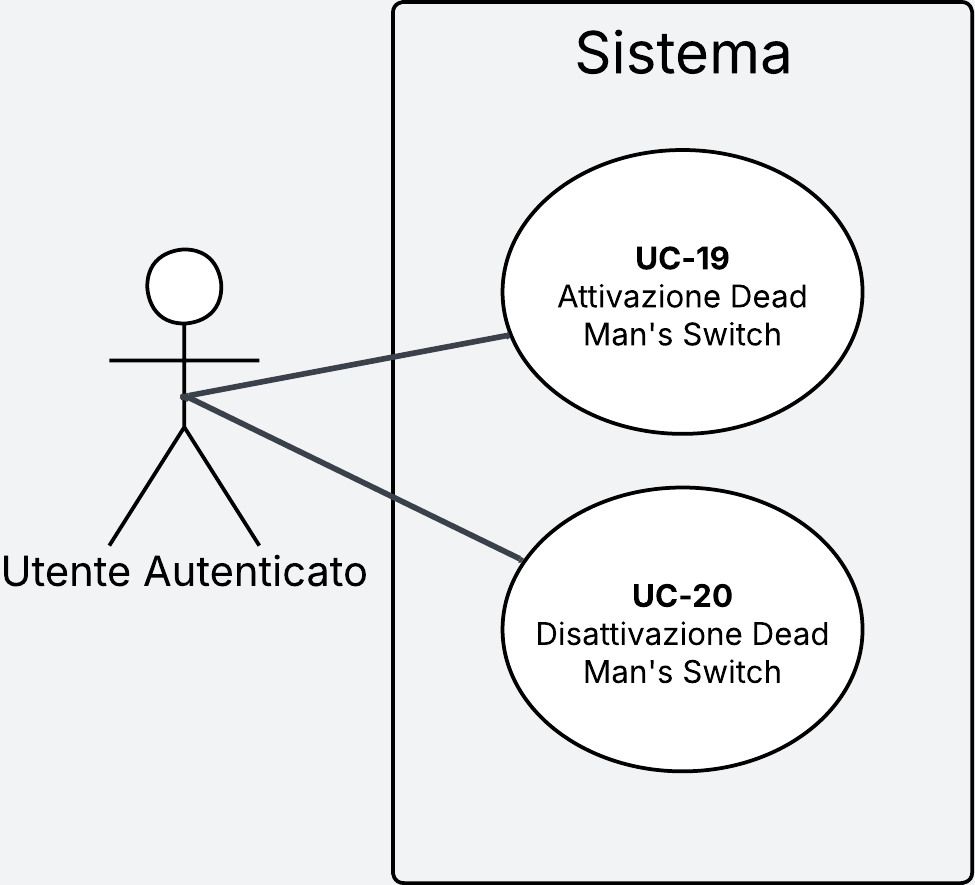
\includegraphics[width=1\textwidth]{use_case/UC-19-20-dmswitch.png}
    \caption{Diagramma dei casi d'uso UC-19 e UC-20}
    \label{fig:UC-19}
\end{figure}
\begin{itemize}
    \item \textbf{Attore principale:} \term{Utente} Autenticato
    \item \textbf{Pre-condizioni:}
    \begin{itemize}
        \item Il sistema è attivo
        \item L'attore ha effettuato l'accesso alle impostazioni del Dead Man's Switch
        \item L'attore ha selezionato l'opzione di attivazione del Dead Man's Switch
    \end{itemize}
    \item \textbf{Post-condizioni:}
    \begin{itemize}
        \item Il Dead Man's Switch è attivo
    \end{itemize}
    \item \textbf{Scenario principale:} 
    \begin{itemize}
        \item L'attore seleziona l'opzione di attivazione del Dead Man's Switch
    \end{itemize}
    \item \textbf{Trigger:} L'attore vuole attivare la funzionalità del Dead Man's Switch
\end{itemize}

\subsubsection{UC-20 - Disattivazione Dead Man's Switch} \label{sec:UC-20}
\begin{itemize}
    \item \textbf{Attore principale:} \term{Utente} Autenticato
    \item \textbf{Pre-condizioni:}
    \begin{itemize}
        \item Il sistema è attivo
        \item L'attore ha effettuato l'accesso alle impostazioni del Dead Man's Switch
        \item L'attore ha selezionato l'opzione di disattivazione del Dead Man's Switch
    \end{itemize}
    \item \textbf{Post-condizioni:}
    \begin{itemize}
        \item Il Dead Man's Switch non è attivo
    \end{itemize}
    \item \textbf{Scenario principale:} 
    \begin{itemize}
        \item L'attore seleziona l'opzione di disattivazione del Dead Man's Switch
    \end{itemize}
    \item \textbf{Trigger:} L'attore vuole disattivare la funzionalità del Dead Man's Switch
\end{itemize}

% ==== DIARIO CRIPTATO =====

\subsubsection{UC-21 - Impostazione password per diario criptato} \label{subsec:UC-21}
\begin{figure}[H]
    \centering
    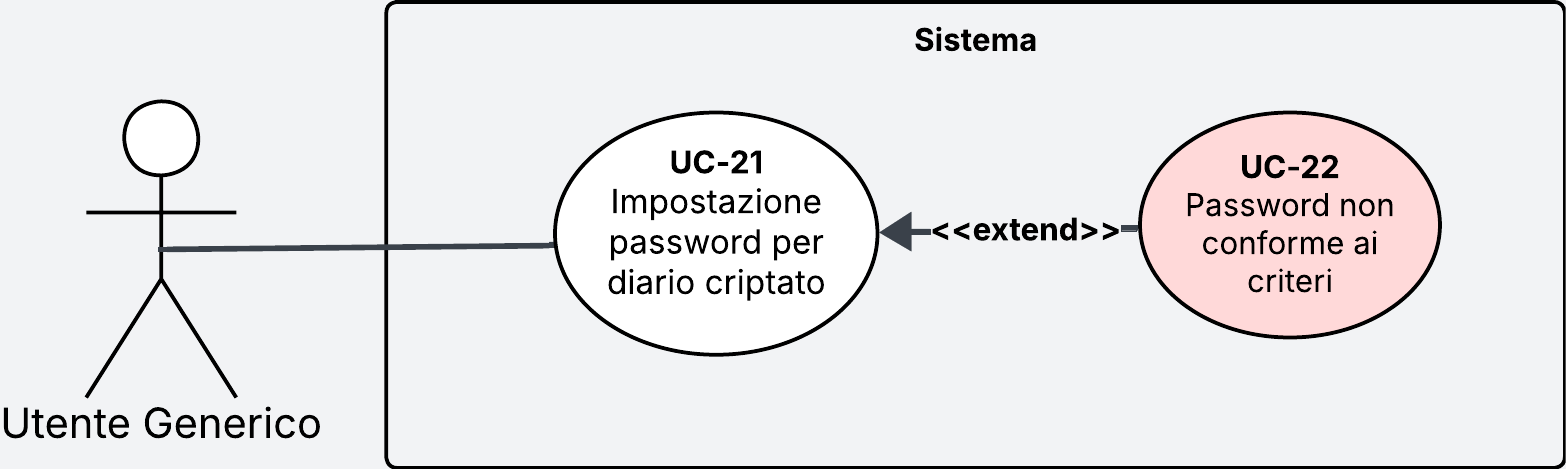
\includegraphics[width=1\textwidth]{use_case/UC-21-impostazione-password-diario-criptato.png}
    \caption{Diagramma del caso d'uso UC-21}
    \label{fig:UC-21}
\end{figure}
\begin{itemize}
    \item \textbf{Attore principale:} \term{Utente} Generico
    \item \textbf{Pre-condizioni:}
    \begin{itemize}
        \item Il sistema è attivo
        \item L'attore si trova nella schermata di impostazione password per il diario criptato
        \item L'attore non ha nessuna password impostata per il diario criptato
    \end{itemize}
    \item \textbf{Post-condizioni:} 
    \begin{itemize}
        \item Il sistema ha validato e memorizzato la password del diario criptato
        \item L'attore è autenticato al diario
    \end{itemize}
    \item \textbf{Scenario principale:} 
    \begin{itemize}
        \item L'attore digita la password desiderata per il diario criptato nel campo dedicato
        \item L'attore conferma l'inserimento della password
        \item Il sistema valida la password inserita
        \item Il sistema memorizza la password del diario criptato
    \end{itemize}
    \item \textbf{Scenari secondari:} 
    \begin{itemize}
        \item La password non è conforme ai criteri di sicurezza minimi imposti dal sistema. La password non viene memorizzata e viene mostrato un messaggio di errore. $\rightarrow$ \hyperref[subsec:UC-22]{UC-22}
    \end{itemize}
    \item \textbf{Estensioni:}
    \begin{itemize}
        \item \hyperref[subsec:UC-22]{UC-22}
    \end{itemize}
    \item \textbf{Trigger:} L'attore vuole impostare la password per il diario criptato
\end{itemize}

\subsubsection{UC-22 - Password non conforme ai criteri} \label{subsec:UC-22}
\begin{itemize}
    \item \textbf{Attore principale:} \term{Utente} Generico
    \item \textbf{Pre-condizioni:}
    \begin{itemize}
        \item Il sistema è attivo
        \item L'attore sta impostando la password per l'accesso al diario
        \item La password inserita non rispetta i criteri di sicurezza definiti dal sistema
    \end{itemize}
    \item \textbf{Post-condizioni:} 
    \begin{itemize}
        \item Il sistema ha notificato l'attore della non conformità
        \item La password non è stata accettata
        \item L'attore può inserire una nuova password conforme ai criteri
    \end{itemize}
    \item \textbf{Scenario principale:} 
    \begin{itemize}
        \item Il sistema valida la password inserita rispetto ai criteri di sicurezza
        \item Il sistema rileva che la password non soddisfa i requisiti minimi
        \item Il sistema visualizza un messaggio di errore specificando i criteri non soddisfatti
        \item Il sistema richiede all'attore di inserire una password valida
    \end{itemize}
    \item \textbf{Trigger:} La password inserita non rispetta i criteri di sicurezza dell'applicazione
\end{itemize}

\subsubsection{UC-23 - Impostazione password per diario fittizio} \label{subsec:UC-23}
\begin{figure}[H]
    \centering
    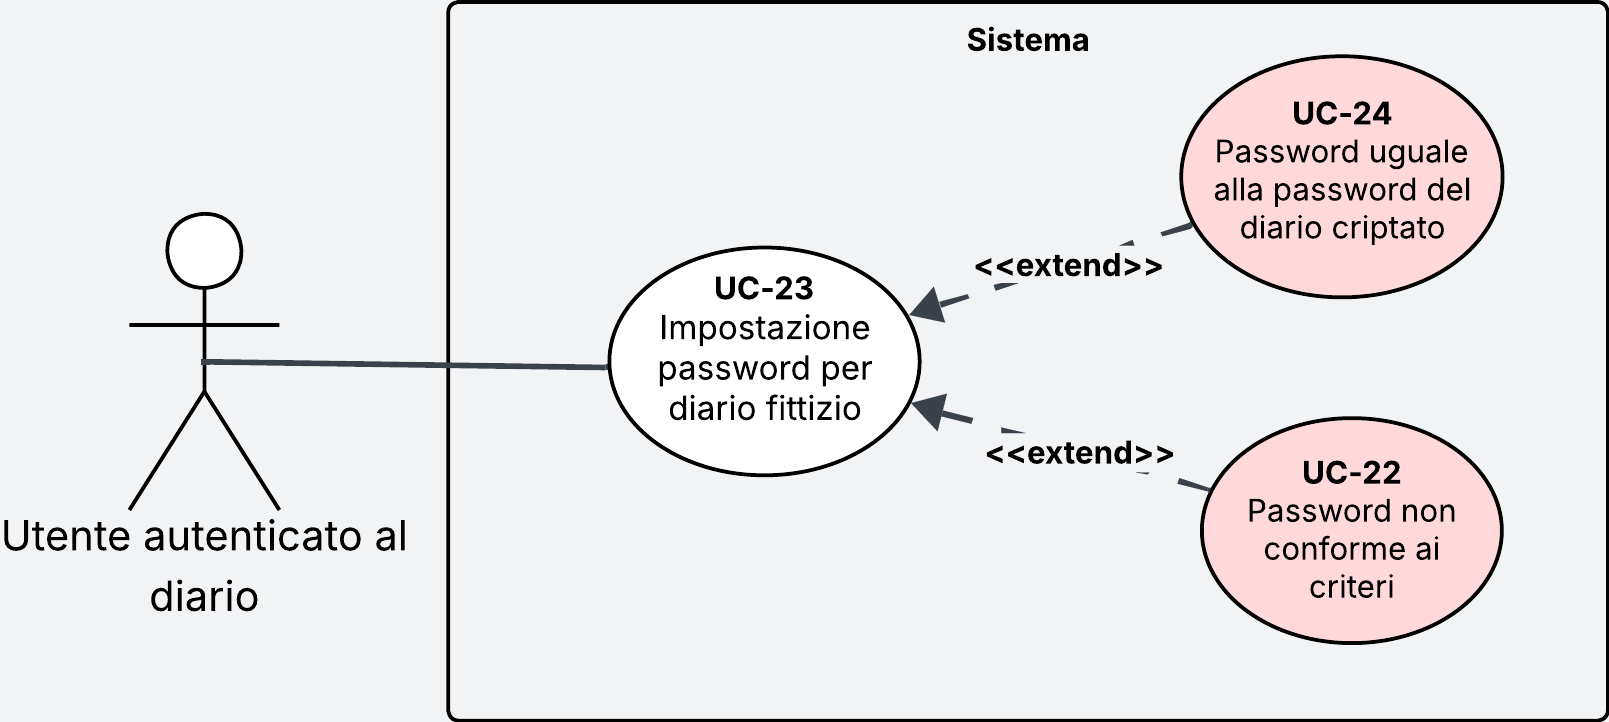
\includegraphics[width=1\textwidth]{use_case/UC-23-impostazione-password-diario-fittizio.png}
    \caption{Diagramma del caso d'uso UC-23}
    \label{fig:UC-23}
\end{figure}
\begin{itemize}
    \item \textbf{Attore principale:} \term{Utente} autenticato al diario
    \item \textbf{Pre-condizioni:}
    \begin{itemize}
        \item Il sistema è attivo
        \item L'attore si trova all'interno del diario criptato
        \item L'attore non ha nessuna password impostata per il diario fittizio
    \end{itemize}
    \item \textbf{Post-condizioni:} 
    \begin{itemize}
        \item La password del diario fittizio è validata e memorizzata
    \end{itemize}
    \item \textbf{Scenario principale:} 
    \begin{itemize}
        \item L'attore seleziona la voce per l'impostazione della password per il diario fittizio
        \item L'attore digita la password desiderata per il diario fittizio nel campo dedicato
        \item L'attore conferma la password inserita
        \item Il sistema valida la password inserita
        \item Il sistema memorizza la password del diario fittizio
    \end{itemize}
    \item \textbf{Scenari secondari:} 
    \begin{itemize}
        \item La password del diario fittizio combacia con quella già impostata del diario criptato. $\rightarrow$ \hyperref[subsec:UC-24]{UC-24}
        \item La password non è conforme ai criteri di sicurezza minimi imposti dal sistema. La password non viene memorizzata e viene mostrato un messaggio di errore. $\rightarrow$ \hyperref[subsec:UC-22]{UC-22}
    \end{itemize}
    \item \textbf{Estensioni:}
    \begin{itemize}
        \item \hyperref[subsec:UC-24]{UC-24}
        \item \hyperref[subsec:UC-22]{UC-22}
    \end{itemize}
    \item \textbf{Trigger:} L'attore vuole impostare la password per il diario fittizio
\end{itemize}

\subsubsection{UC-24 - Password uguale alla password del diario criptato} \label{subsec:UC-24}
\begin{itemize}
    \item \textbf{Attore principale:} \term{Utente} autenticato al diario
    \item \textbf{Pre-condizioni:}
    \begin{itemize}
        \item Il sistema è attivo
        \item L'attore sta impostando la password per il diario fittizio
        \item La password inserita è identica alla password del diario criptato
    \end{itemize}
    \item \textbf{Post-condizioni:} 
    \begin{itemize}
        \item Il sistema ha notificato l'attore dell'errore
        \item La password non è stata memorizzata
        \item L'attore può inserire una nuova password
    \end{itemize}
    \item \textbf{Scenario principale:} 
    \begin{itemize}
        \item Il sistema rileva che la password inserita è identica a quella del diario criptato
        \item Il sistema visualizza un messaggio di errore informando l'attore che le due password devono essere differenti
        \item Il sistema richiede all'attore di inserire una password diversa
    \end{itemize}
    \item \textbf{Trigger:} La password inserita per il diario fittizio corrisponde alla password del diario criptato
\end{itemize}

\subsubsection{UC-25 - Inserimento password accesso diario} \label{subsec:UC-25}
\begin{figure}[H]
    \centering
    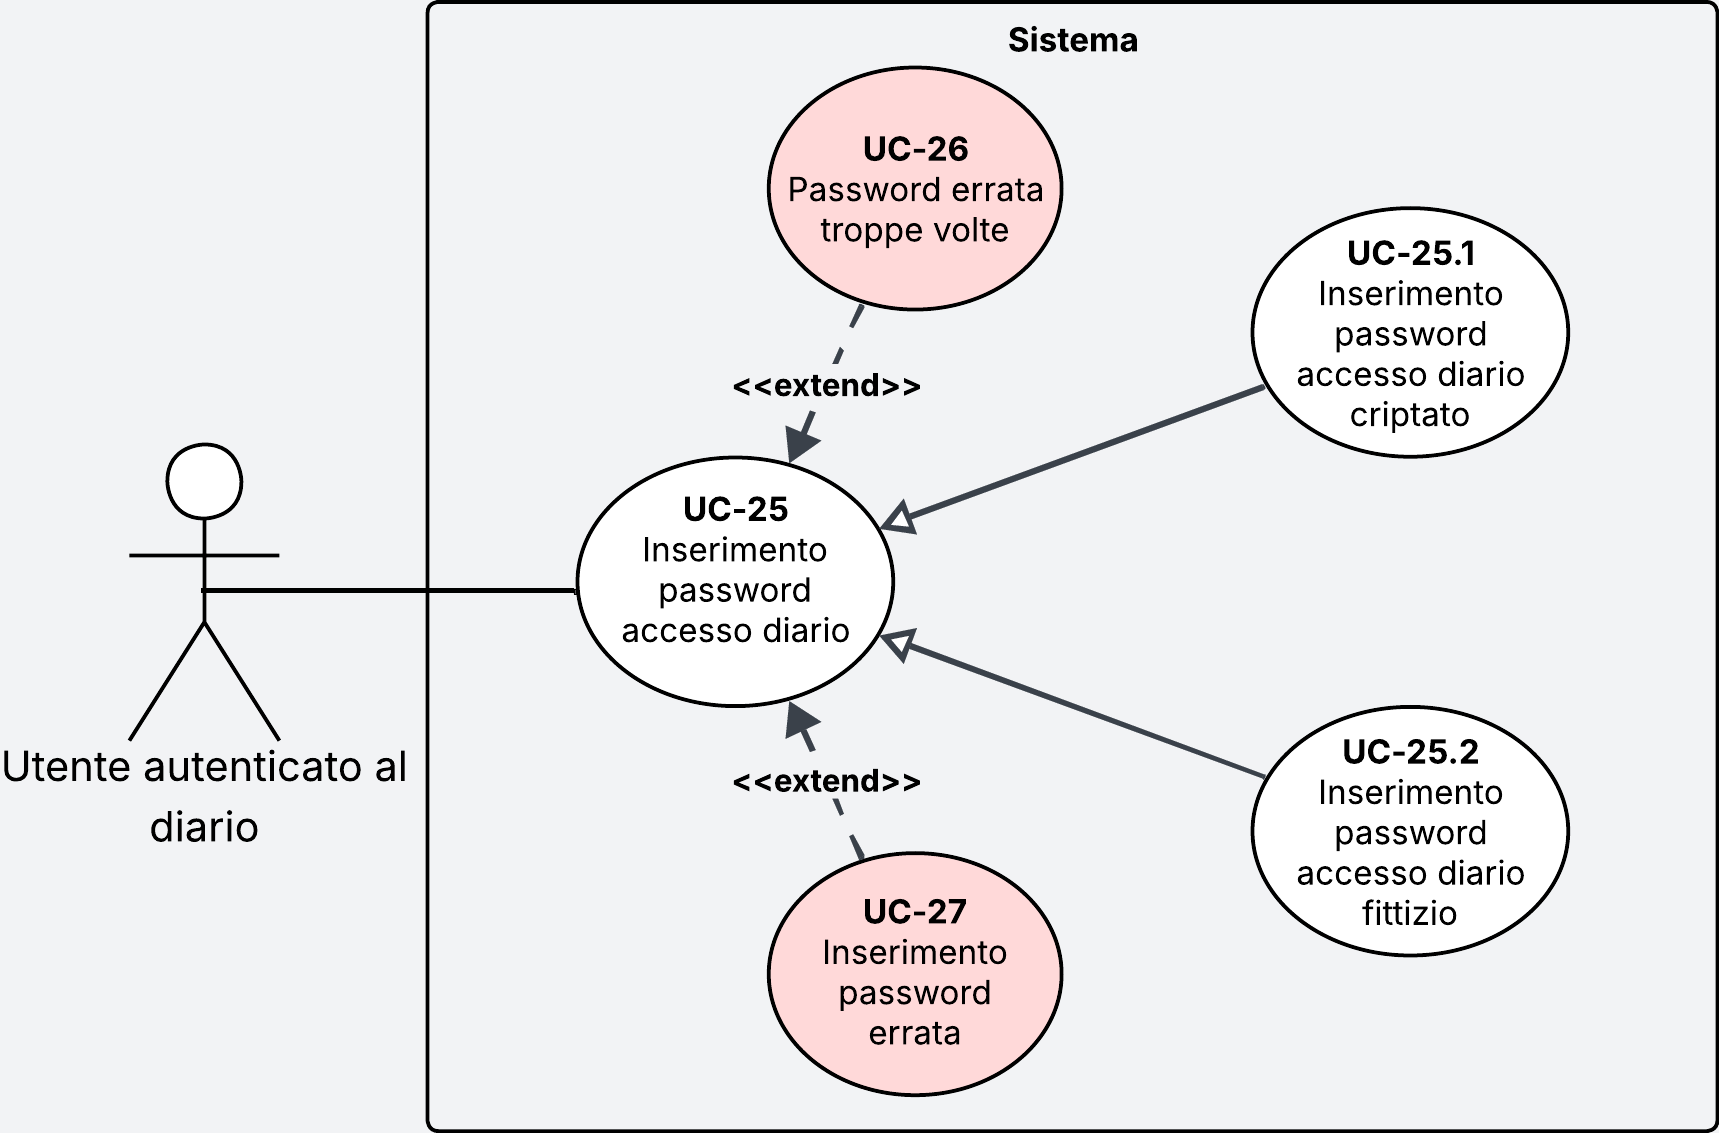
\includegraphics[width=1\textwidth]{use_case/UC-25-inserimento-password-accesso-diario.png}
    \caption{Diagramma del caso d'uso UC-25}
    \label{fig:UC-25}
\end{figure}
\begin{itemize}
    \item \textbf{Attore principale:} \term{Utente} autenticato al diario
    \item \textbf{Pre-condizioni:}
    \begin{itemize}
        \item Il sistema è attivo
        \item L'attore si trova nella schermata di accesso al diario
    \end{itemize}
    \item \textbf{Post-condizioni:} 
    \begin{itemize}
        \item L'attore ha accesso al diario corrispondente alla password inserita
    \end{itemize}
    \item \textbf{Scenario principale:} 
    \begin{itemize}
        \item L'attore inserisce la password nel campo dedicato
        \item L'attore conferma l'inserimento
        \item Il sistema riceve la password inserita e \ignoreglossary{verifica} che corrisponda a una delle password memorizzate
        \item L'attore ottiene l'accesso al diario a cui corrisponde la password inserita
    \end{itemize}
    \item \textbf{Scenari secondari:} 
    \begin{itemize}
        \item L'attore inserisce la password errata. Il sistema notifica l'errore e impedisce l'accesso al diario. $\rightarrow$ \hyperref[subsec:UC-27]{UC-27}
        \item L'attore ha inserito la password errata più volte di quanto consentito dal sistema. Il sistema nega l'accesso e disabilita l'inserimento della password per un periodo di tempo predefinito. $\rightarrow$ \hyperref[subsec:UC-26]{UC-26}
    \end{itemize}
    \item \textbf{Estensioni:}
    \begin{itemize}
        \item \hyperref[subsec:UC-27]{UC-27}
        \item \hyperref[subsec:UC-26]{UC-26}
    \end{itemize}
        \item \textbf{Trigger:} L'attore vuole accedere al diario
        \item \textbf{Specializzazioni:}
    \begin{itemize}
        \item \hyperref[subsec:UC-25.1]{UC-25.1}
        \item \hyperref[subsec:UC-25.2]{UC-25.2}
    \end{itemize}

\end{itemize}

\subsubsection{UC-25.1 - Inserimento password accesso diario criptato} \label{subsec:UC-25.1}
\begin{itemize}
    \item \textbf{Attore principale:} \term{Utente} autenticato al diario
    \item \textbf{Pre-condizioni:}
    \begin{itemize}
        \item Il sistema è attivo
        \item L'attore si trova nella schermata di accesso al diario
    \end{itemize}
    \item \textbf{Post-condizioni:} 
    \begin{itemize}
        \item L'attore ha accesso al diario criptato
    \end{itemize}
    \item \textbf{Scenario principale:} 
    \begin{itemize}
        \item L'attore inserisce la password nel campo dedicato
        \item L'attore conferma l'inserimento
        \item Il sistema riceve la password e \ignoreglossary{verifica} che corrisponda alla password memorizzata per il diario criptato
        \item L'attore ottiene l'accesso al diario criptato
    \end{itemize}

\end{itemize}

\subsubsection{UC-25.2 - Inserimento password accesso diario fittizio} \label{subsec:UC-25.2}
\begin{itemize}
    \item \textbf{Attore principale:} \term{Utente} autenticato al diario
    \item \textbf{Pre-condizioni:}
    \begin{itemize}
        \item Il sistema è attivo
        \item L'attore si trova nella schermata di accesso al diario
        \item Il diario fittizio è stato precedentemente configurato con una password
    \end{itemize}
    \item \textbf{Post-condizioni:} 
    \begin{itemize}
        \item L'attore ha accesso al diario fittizio
    \end{itemize}
    \item \textbf{Scenario principale:} 
    \begin{itemize}
        \item L'attore inserisce la password nel campo dedicato
        \item L'attore conferma l'inserimento
        \item Il sistema riceve la password e \ignoreglossary{verifica} che corrisponda alla password memorizzata per il diario fittizio
        \item L'attore ottiene l'accesso al diario fittizio
    \end{itemize}

\end{itemize}

\subsubsection{UC-26 - Password errata troppe volte} \label{subsec:UC-26}
\begin{itemize}
    \item \textbf{Attore principale:} \term{Utente} autenticato al diario
    \item \textbf{Pre-condizioni:}
    \begin{itemize}
        \item Il sistema è attivo
        \item L'attore si trova nella schermata di accesso al diario
        \item L'attore ha effettuato molteplici tentativi falliti di accesso al diario
        \item Il numero di tentativi errati ha superato la soglia massima consentita
    \end{itemize}
    \item \textbf{Post-condizioni:} 
    \begin{itemize}
        \item Il sistema ha attivato le misure di sicurezza previste
        \item L'accesso al diario è temporaneamente bloccato
    \end{itemize}
    \item \textbf{Scenario principale:} 
    \begin{itemize}
        \item Il sistema rileva il superamento del numero massimo di tentativi falliti
        \item Il sistema blocca temporaneamente l'accesso alla funzionalità del diario
        \item Il sistema visualizza un messaggio informando l'attore del blocco temporaneo
        \item Il sistema attende un periodo di tempo predefinito prima di consentire nuovi tentativi
    \end{itemize}
    \item \textbf{Trigger:} L'attore ha inserito la password errata per un numero di volte superiore alla soglia massima consentita
\end{itemize}

\subsubsection{UC-27 - Inserimento password errata} \label{subsec:UC-27}
\begin{itemize}
    \item \textbf{Attore principale:} \term{Utente} autenticato al diario
    \item \textbf{Pre-condizioni:}
    \begin{itemize}
        \item Il sistema è attivo
        \item L'attore si trova nella schermata di accesso al diario
        \item L'attore ha inserito una password per l'accesso al diario
        \item La password inserita non corrisponde né a quella del diario criptato, né a quella del diario fittizio
        \item Il numero di tentativi errati non ha superato la soglia massima consentita
    \end{itemize}
    \item \textbf{Post-condizioni:} 
    \begin{itemize}
        \item Il sistema registra l'avvenuto inserimento di una password errata
        \item Il sistema ha negato l'accesso al diario
        \item L'attore può effettuare un nuovo tentativo di accesso
    \end{itemize}
    \item \textbf{Scenario principale:} 
    \begin{itemize}
        \item Il sistema rileva che la password inserita non corrisponde a nessuna tra le password memorizzate
        \item Il sistema visualizza un messaggio di errore informando l'attore dell'inserimento errato
    \end{itemize}
    \item \textbf{Trigger:} L'attore inserisce una password errata per l'accesso al diario

\end{itemize}

\subsubsection{UC-28 - Visualizzazione diario criptato} \label{subsec:UC-28}
\begin{figure}[H]
    \centering
    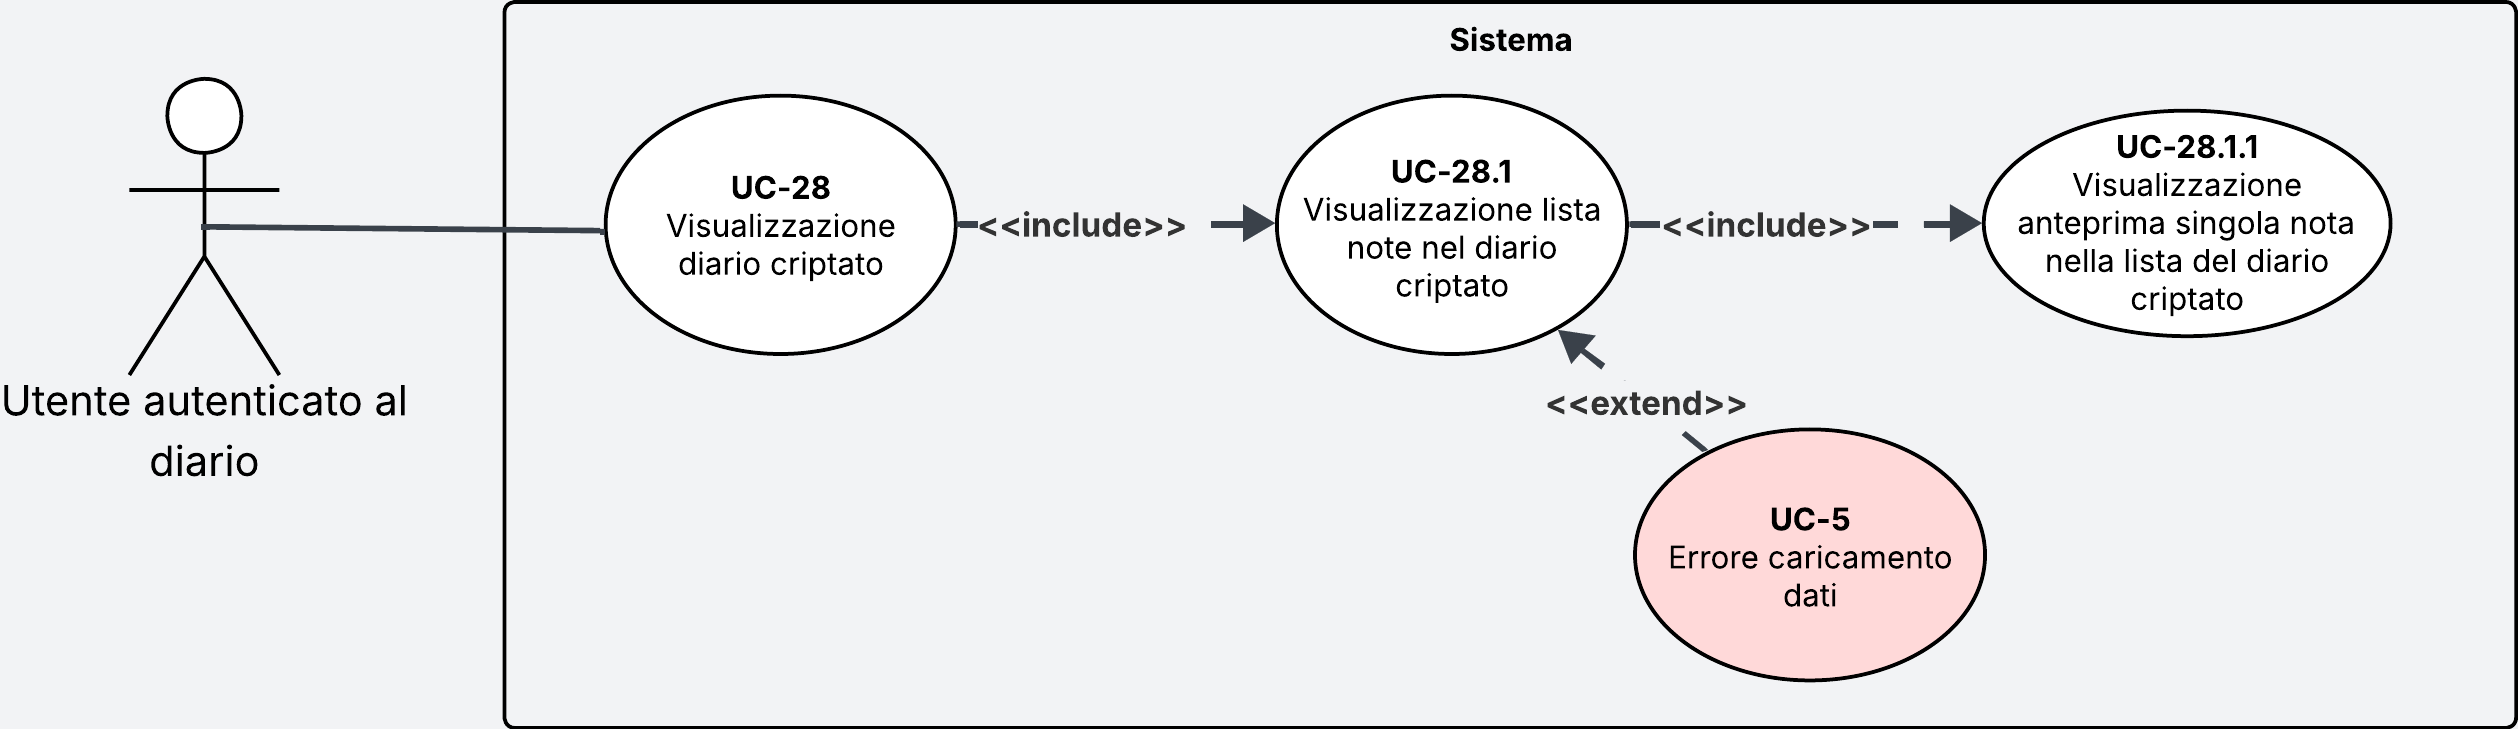
\includegraphics[width=1\textwidth]{use_case/UC-28-visualizzazione-diario-criptato.png}
    \caption{Diagramma del caso d'uso UC-28}
    \label{fig:UC-28}
\end{figure}
\begin{itemize}
    \item \textbf{Attore principale:} \term{Utente} autenticato al diario
    \item \textbf{Pre-condizioni:}
    \begin{itemize}
        \item Il sistema è attivo
        \item L'attore si trova all'interno del diario criptato
    \end{itemize}
    \item \textbf{Post-condizioni:} 
    \begin{itemize}
        \item Il sistema visualizza l'interfaccia principale del diario criptato con la lista delle note
    \end{itemize}
    \item \textbf{Scenario principale:} 
    \begin{itemize}
        \item L'attore accede alla schermata principale del diario criptato
        \item Il sistema carica e visualizza la lista delle note presenti $\rightarrow$ \hyperref[subsec:UC-28.1]{UC-28.1}
    \end{itemize}
    \item \textbf{Inclusioni:}
    \begin{itemize}
        \item \hyperref[subsec:UC-28.1]{UC-28.1}
    \end{itemize}
    \item \textbf{Trigger:} L'attore vuole accedere al diario criptato
\end{itemize}

\subsubsection{UC-28.1 - Visualizzazione lista note nel diario criptato} \label{subsec:UC-28.1}
\begin{itemize}
    \item \textbf{Attore principale:} \term{Utente} autenticato al diario
    \item \textbf{Pre-condizioni:}
    \begin{itemize}
        \item Il sistema è attivo
        \item L'attore si trova all'interno del diario criptato
        \item Esiste almeno una nota all'interno del diario criptato
    \end{itemize}
    \item \textbf{Post-condizioni:} 
    \begin{itemize}
        \item Il sistema visualizza l'elenco completo delle anteprime delle note presenti nel diario criptato
    \end{itemize}
    \item \textbf{Scenario principale:} 
    \begin{itemize}
        \item Il sistema recupera tutte le note memorizzate nel diario criptato
        \item Il sistema visualizza, in una lista, le anteprime di ogni singola nota $\rightarrow$ \hyperref[subsec:UC-28.1.1]{UC-28.1.1}
    \end{itemize}
    \item \textbf{Scenario secondario:} 
    \begin{itemize}
        \item Il sistema non è in grado di recuperare le note dal database $\rightarrow$ \hyperref[sec:UC-5]{UC-5}
    \end{itemize}
    \item \textbf{Inclusioni:}
    \begin{itemize}
        \item \hyperref[subsec:UC-28.1.1]{UC-28.1.1}
    \end{itemize}
    \item \textbf{Estensioni:}
    \begin{itemize}
        \item \hyperref[sec:UC-5]{UC-5}
    \end{itemize}
    \item \textbf{Trigger:} L'attore vuole accedere al diario criptato
\end{itemize}

\subsubsection{UC-28.1.1 - Visualizzazione anteprima singola nota della lista nel diario criptato} \label{subsec:UC-28.1.1}
\begin{itemize}
    \item \textbf{Attore principale:} \term{Utente} autenticato al diario
    \item \textbf{Pre-condizioni:}
    \begin{itemize}
        \item Il sistema è attivo
        \item L'attore si trova all'interno del diario criptato
        \item Esiste almeno una nota all'interno del diario criptato
        \item L'attore sta visualizzando la sezione contenente la lista delle note del diario criptato
        \item Il sistema ha recuperato e organizzato le anteprime delle note da visualizzare
    \end{itemize}
    \item \textbf{Post-condizioni:} 
    \begin{itemize}
        \item Il sistema visualizza l'anteprima di una nota all'interno della lista
    \end{itemize}
    \item \textbf{Scenario principale:} 
    \begin{itemize}
        \item Il sistema recupera le informazioni della nota da visualizzare
        \item Il sistema visualizza parte del contenuto testuale presente all'inizio della nota
    \end{itemize}
    \item \textbf{Trigger:} L'attore vuole accedere al diario criptato
\end{itemize}

% UC modifica e visualizzazione note diario criptato
\subsubsection{UC-30 - Eliminazione nota diario criptato} \label{subsec:UC-30}
\begin{figure}[H]
    \centering
    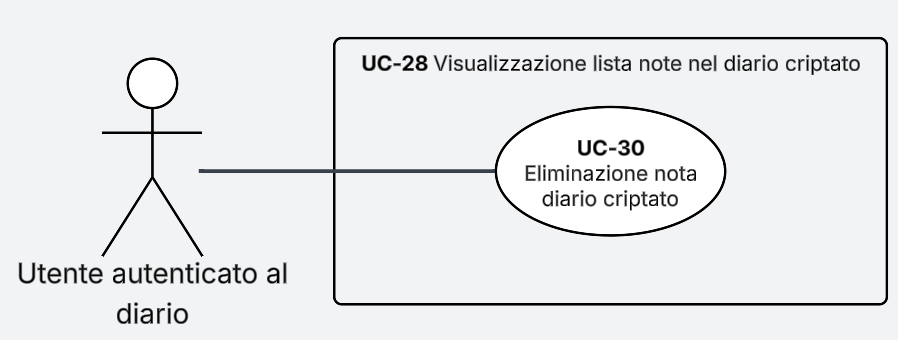
\includegraphics[width=1\textwidth]{use_case/UC-30-diario.png}
    \caption{Diagramma dei casi d'uso UC-30 e UC-30.1}
    \label{fig:UC-30, UC-30.1}
\end{figure}
\begin{itemize}
    \item \textbf{Attore principale:} \term{Utente} Autenticato al diario
    \item \textbf{Pre-condizioni:}
    \begin{itemize}
        \item Il sistema è attivo
        \item L'attore è all'interno del diario criptato
        \item Esiste almeno una nota nel diario criptato
        \item L'attore sta visualizzando la lista delle note del diario criptato
    \end{itemize}
    \item \textbf{Post-condizioni:} 
    \begin{itemize}
        \item La nota è stata rimossa dal diario criptato
        \item La nota non è più visibile nella lista delle note del diario criptato
    \end{itemize}
    \item \textbf{Scenario principale:} 
    \begin{itemize}
        \item L'attore seleziona la voce di eliminazione di una nota dalla lista di note del diario criptato
        \item Il sistema richiede conferma dell'operazione di eliminazione $\rightarrow$ \hyperref[subsec:UC-30.1]{UC-30.1}
        \item L'attore conferma l'eliminazione
        \item Il sistema rimuove definitivamente la nota dal diario criptato
        \item Il sistema aggiorna la lista delle note
    \end{itemize}
    \item \textbf{Inclusioni:}
    \begin{itemize}
        \item \hyperref[subsec:UC-30.1]{UC-30.1}
    \end{itemize}
    \item \textbf{Trigger:} L'attore desidera eliminare una nota del diario criptato
\end{itemize}

\subsubsection{UC-30.1 - Conferma eliminazione nota diario criptato}\label{subsec:UC-30.1}
\begin{itemize}
    \item \textbf{Attore principale:} \term{Utente} autenticato al diario
    \item \textbf{Pre-condizioni:}
    \begin{itemize}
        \item Il sistema è attivo
        \item L'attore è all'interno del diario criptato
        \item Esiste almeno una nota nel diario criptato
        \item L'attore sta visualizzando la lista delle note del diario criptato
        \item L'attore ha selezionato la voce per eliminare la nota dalla lista delle note del diario criptato
    \end{itemize}
    \item \textbf{Post-condizioni:}
    \begin{itemize}
        \item Il sistema riceve la conferma dell'attore di eliminare la nota dalla lista delle note del diario criptato
    \end{itemize}
    \item \textbf{Scenario principale:}
    \begin{itemize}
        \item L'attore conferma l'eliminazione di una nota dalla lista di note del diario criptato
        \item Il sistema rimuove la nota dalla lista delle note del diario criptato
    \end{itemize}
    \item \textbf{Trigger:} L'attore desidera eliminare una nota del diario criptato
\end{itemize}

\subsubsection{UC-31 - Creazione nota} \label{subsec:UC-31}
\begin{figure}[H]
    \centering
    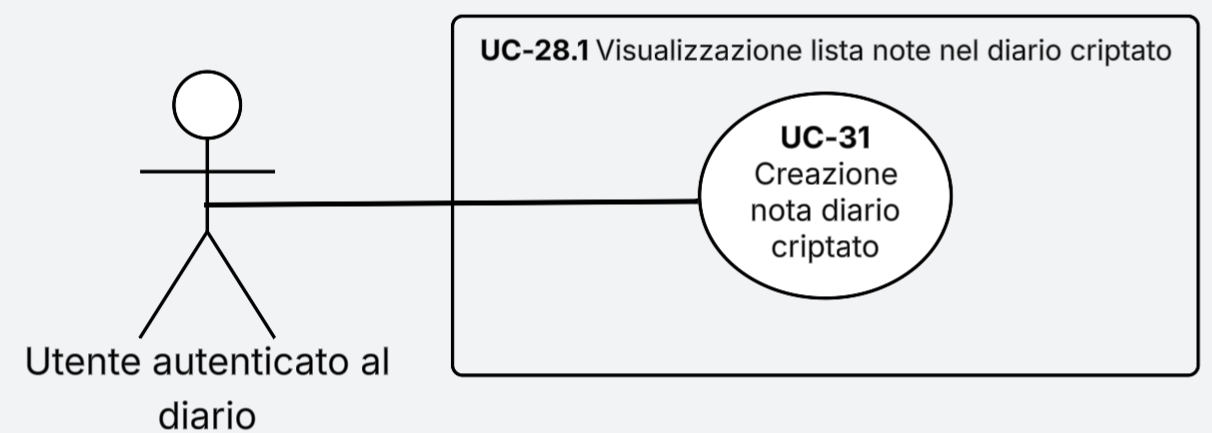
\includegraphics[width=1\textwidth]{use_case/UC-31-diario.png}
    \caption{Diagramma del caso d'uso UC-31}
    \label{fig:UC-31}
\end{figure}
\begin{itemize}
    \item \textbf{Attore principale:} \term{Utente} Autenticato al diario
    \item \textbf{Pre-condizioni:}
    \begin{itemize}
        \item Il sistema è attivo
        \item L'attore si trova all'interno del diario criptato
        \item L'attore sta visualizzando la lista delle note del diario criptato
    \end{itemize}
    \item \textbf{Post-condizioni:} 
    \begin{itemize}
        \item Il sistema crea una nuova nota vuota e la memorizza nel diario criptato
    \end{itemize}
    \item \textbf{Scenario principale:} 
    \begin{itemize}
        \item L'attore ha selezionato la voce per l'aggiunta di una nuova nota
        \item La nuova nota viene creata ed è visibile nella lista delle note del diario criptato
    \end{itemize}
    \item \textbf{Trigger:} L'attore vuole creare una nuova nota nel diario criptato
\end{itemize}

\subsubsection{UC-32 - Visualizzazione contenuto nota diario criptato} \label{subsec:UC-32}
\begin{figure}[H]
    \centering
    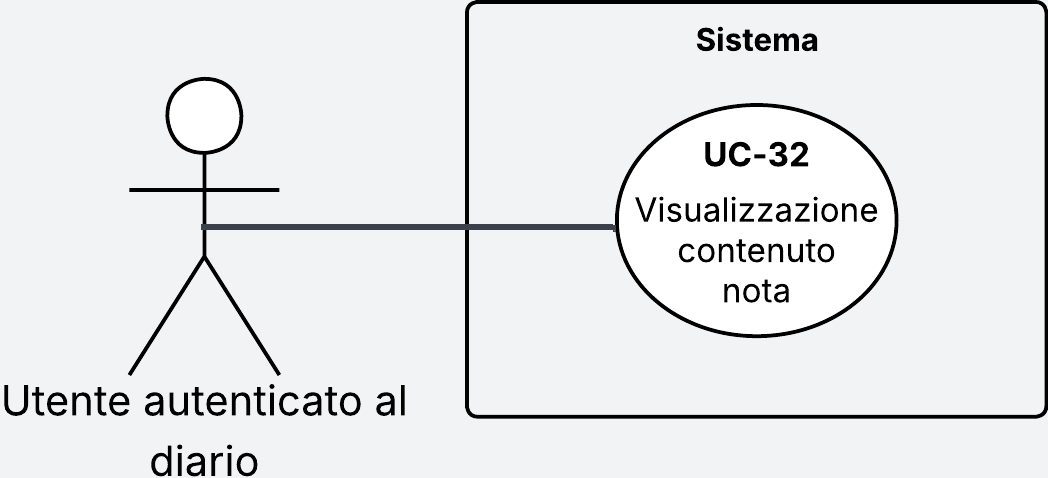
\includegraphics[width=1\textwidth]{use_case/UC-32-diario.png}
    \caption{Diagramma del caso d'uso UC-32}
    \label{fig:UC-32}
\end{figure}
\begin{itemize}
    \item \textbf{Attore principale:} \term{Utente} Autenticato al diario
    \item \textbf{Pre-condizioni:}
    \begin{itemize}
        \item Il sistema è attivo
        \item L'attore si trova all'interno del diario criptato
        \item Esiste almeno una nota nel diario criptato
        \item L'attore sta visualizzando la lista delle note nel diario criptato
    \end{itemize}
    \item \textbf{Post-condizioni:} 
    \begin{itemize}
        \item L'attore visualizza il contenuto di una nota del diario criptato
    \end{itemize}
    \item \textbf{Scenario principale:} 
    \begin{itemize}
        \item L'attore seleziona una nota dalla lista
        \item Il sistema recupera il contenuto completo della nota
        \item Il sistema visualizza a schermo il contenuto testuale della nota $\rightarrow$ \hyperref[subsec:UC-32.1]{UC-32.1}
        \item Il sistema visualizza a schermo il contenuto multimediale della nota $\rightarrow$ \hyperref[subsec:UC-32.2]{UC-32.2}
        \item L'attore può visualizzare e interagire con il contenuto della nota
    \end{itemize}
    \item \textbf{Inclusioni:}
    \begin{itemize}
        \item \hyperref[subsec:UC-32.1]{UC-32.1}
        \item \hyperref[subsec:UC-32.2]{UC-32.2}
    \end{itemize}
    \item \textbf{Trigger:} L'attore vuole visualizzare il contenuto di una nota nel diario criptato
\end{itemize}

\subsubsection{UC-32.1 - Visualizzazione contenuto testuale nota diario criptato} \label{subsec:UC-32.1}
\begin{itemize}
    \item \textbf{Attore principale:} \term{Utente} Autenticato al diario
    \item \textbf{Pre-condizioni:}
    \begin{itemize}
        \item Il sistema è attivo
        \item L'attore si trova all'interno del diario criptato
        \item Esiste almeno una nota nel diario criptato
        \item L'attore sta visualizzando il contenuto di una nota del diario criptato
    \end{itemize}
    \item \textbf{Post-condizioni:}
    \begin{itemize}
        \item L'attore visualizza il contenuto testuale della nota
    \end{itemize}
    \item \textbf{Scenario principale:}
    \begin{itemize}
        \item Il sistema mostra il contenuto testuale della nota 
    \end{itemize}
    \item \textbf{Trigger:} L'attore vuole visualizzare il contenuto testuale di una nota del diario criptato
\end{itemize}

\subsubsection{UC-32.2 - Visualizzazione contenuto multimediale nota diario criptato} \label{subsec:UC-32.2}
\begin{itemize}
    \item \textbf{Attore principale:} \term{Utente} Autenticato al diario
    \item \textbf{Pre-condizioni:}
    \begin{itemize}
        \item Il sistema è attivo
        \item L'attore si trova all'interno del diario criptato
        \item Esiste almeno una nota nel diario criptato
        \item L'attore sta visualizzando il contenuto di una nota del diario criptato
    \end{itemize}
    \item \textbf{Post-condizioni:}
    \begin{itemize}
        \item L'attore visualizza il contenuto multimediale della nota
    \end{itemize}
    \item \textbf{Scenario principale:}
    \begin{itemize}
        \item Il sistema mostra il contenuto multimediale della nota 
    \end{itemize}
    \item \textbf{Specializzazioni:}
    \begin{itemize}
        \item \hyperref[subsec:UC-32.2.1]{UC-32.2.1}
        \item \hyperref[subsec:UC-32.2.2]{UC-32.2.2}
    \end{itemize}
    \item \textbf{Trigger:} L'attore vuole visualizzare il contenuto multimediale di una nota del diario criptato
\end{itemize}

\subsubsection{UC-32.2.1 - Visualizzazione audio nota diario criptato} \label{subsec:UC-32.2.1}
\begin{itemize}
    \item \textbf{Attore principale:} \term{Utente} Autenticato al diario
    \item \textbf{Pre-condizioni:}
    \begin{itemize}
        \item Il sistema è attivo
        \item L'attore si trova all'interno del diario criptato
        \item Esiste almeno una nota nel diario criptato
        \item L'attore sta visualizzando il contenuto di una nota del diario criptato
    \end{itemize}
    \item \textbf{Post-condizioni:}
    \begin{itemize}
        \item L'attore visualizza il contenuto audio presente nella nota
    \end{itemize}
    \item \textbf{Scenario principale:}
    \begin{itemize}
        \item Il sistema mostra il contenuto audio presente nella nota 
    \end{itemize}
    \item \textbf{Trigger:} L'attore vuole visualizzare il contenuto audio di una nota del diario criptato
\end{itemize}

\subsubsection{UC-32.2.2 - Visualizzazione immagini nota diario criptato} \label{subsec:UC-32.2.2}
\begin{itemize}
    \item \textbf{Attore principale:} \term{Utente} Autenticato al diario
    \item \textbf{Pre-condizioni:}
    \begin{itemize}
        \item Il sistema è attivo
        \item L'attore si trova all'interno del diario criptato
        \item Esiste almeno una nota nel diario criptato
        \item L'attore sta visualizzando il contenuto di una nota del diario criptato
    \end{itemize}
    \item \textbf{Post-condizioni:}
    \begin{itemize}
        \item L'attore visualizza le immagini presenti nella nota
    \end{itemize}
    \item \textbf{Scenario principale:}
    \begin{itemize}
        \item Il sistema mostra le immagini presenti nella nota 
    \end{itemize}
    \item \textbf{Trigger:} L'attore vuole visualizzare le immagini presenti in una nota del diario criptato
\end{itemize}

\subsubsection{UC-33 - Inserimento testo in nota diario criptato} \label{subsec:UC-33}
\begin{figure}[H]
    \centering
    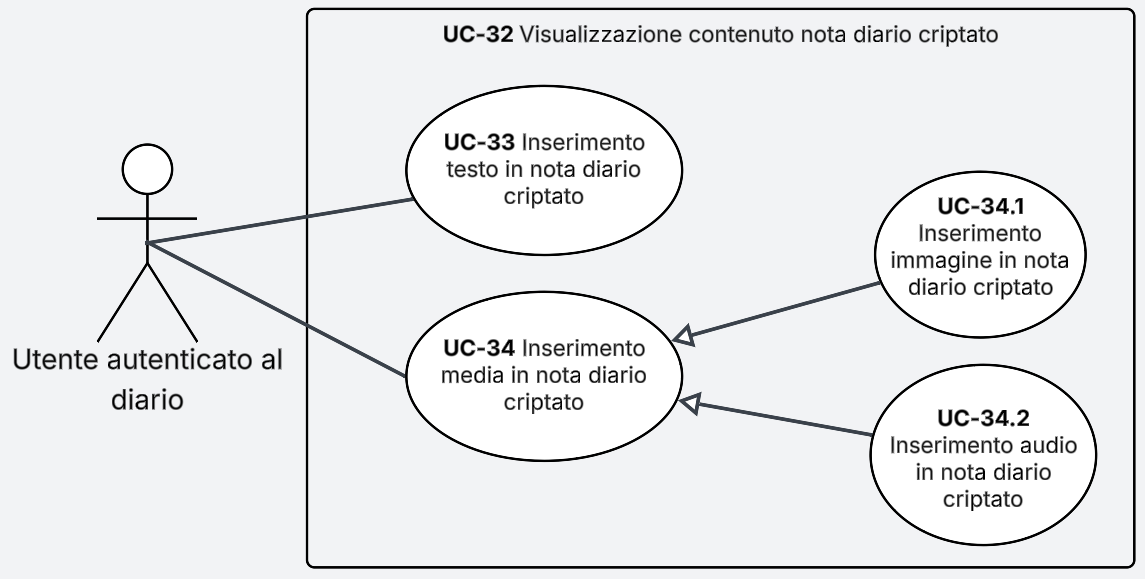
\includegraphics[width=1\textwidth]{use_case/UC-33_32-diario.png}
    \caption{Diagramma dei casi d'uso UC-33, UC-34, UC-34.1 e UC-34.2}
    \label{fig:UC-33, UC-34, UC-34.1, UC-34.2}
\end{figure}
\begin{itemize}
    \item \textbf{Attore principale:} \term{Utente} Autenticato al diario
    \item \textbf{Pre-condizioni:}
    \begin{itemize}
        \item Il sistema è attivo
        \item L'attore si trova all'interno del diario criptato
        \item L'attore sta visualizzando il contenuto di una nota del diario criptato
        \item Non è presente contenuto testuale nella nota
    \end{itemize}
    \item \textbf{Post-condizioni:}
    \begin{itemize}
        \item Il sistema riceve correttamente il testo digitato da memorizzare nella nota
    \end{itemize}
    \item \textbf{Scenario principale:}
    \begin{itemize}
        \item L'attore ha selezionato l'area apposita per l'inserimento del testo nella nota
        \item L'attore digita il testo da inserire nella nota
    \end{itemize}
    \item \textbf{Trigger:} L'attore vuole aggiungere del testo ad una nota nel diario criptato
\end{itemize}

\subsubsection{UC-34 - Inserimento media in nota diario criptato} \label{subsec:UC-34}
\begin{itemize}
    \item \textbf{Attore principale:} \term{Utente} Autenticato al diario
    \item \textbf{Pre-condizioni:}
    \begin{itemize}
        \item Il sistema è attivo
        \item L'attore si trova all'interno del diario criptato
        \item L'attore sta visualizzando il contenuto di una nota del diario criptato
    \end{itemize}
    \item \textbf{Post-condizioni:}
    \begin{itemize}
        \item Il sistema riceve correttamente il media da memorizzare nella nota
    \end{itemize}
    \item \textbf{Scenario principale:}
    \begin{itemize}
        \item L'attore ha selezionato la voce per l'aggiunta di un media
        \item L'attore inserisce il media desiderato
    \end{itemize}
    \item \textbf{Specializzazioni}
    \begin{itemize}
        \item \hyperref[subsec:UC-34.1]{UC-34.1}
        \item \hyperref[subsec:UC-34.2]{UC-34.2}
    \end{itemize}
    \item \textbf{Trigger:} L'attore vuole aggiungere del contenuto multimediale ad una nota nel diario criptato
\end{itemize}

\subsubsection{UC-34.1 - Inserimento immagine in nota diario criptato} \label{subsec:UC-34.1}
\begin{itemize}
    \item \textbf{Attore principale:} \term{Utente} Autenticato al diario
    \item \textbf{Pre-condizioni:}
    \begin{itemize}
        \item Il sistema è attivo
        \item L'attore si trova all'interno del diario criptato
        \item L'attore sta visualizzando il contenuto di una nota del diario criptato
    \end{itemize}
    \item \textbf{Post-condizioni:}
    \begin{itemize}
        \item Il sistema riceve correttamente l'immagine da memorizzare nella nota
    \end{itemize}
    \item \textbf{Scenario principale:}
    \begin{itemize}
        \item L'attore ha selezionato la voce per l'aggiunta di un media
        \item L'attore inserisce una immagine nella nota
    \end{itemize}
    \item \textbf{Trigger:} L'attore vuole aggiungere un'immagine ad una nota nel diario criptato
\end{itemize}

\subsubsection{UC-34.2 - Inserimento audio in nota diario criptato} \label{subsec:UC-34.2}
\begin{itemize}
    \item \textbf{Attore principale:} \term{Utente} Autenticato al diario
    \item \textbf{Pre-condizioni:}
    \begin{itemize}
        \item Il sistema è attivo
        \item L'attore si trova all'interno del diario criptato
        \item L'attore sta visualizzando il contenuto di una nota del diario criptato
    \end{itemize}
    \item \textbf{Post-condizioni:}
    \begin{itemize}
        \item Il sistema riceve correttamente l'audio da memorizzare nella nota
    \end{itemize}
    \item \textbf{Scenario principale:}
    \begin{itemize}
        \item L'attore ha selezionato la voce per l'aggiunta di un media
        \item L'attore inserisce un audio nella nota
    \end{itemize}
    \item \textbf{Trigger:} L'attore vuole aggiungere del contenuto audio ad una nota nel diario criptato
\end{itemize}

\subsubsection{UC-35 - Modifica testo in nota diario criptato} \label{subsec:UC-35}
\begin{figure}[H]
    \centering
    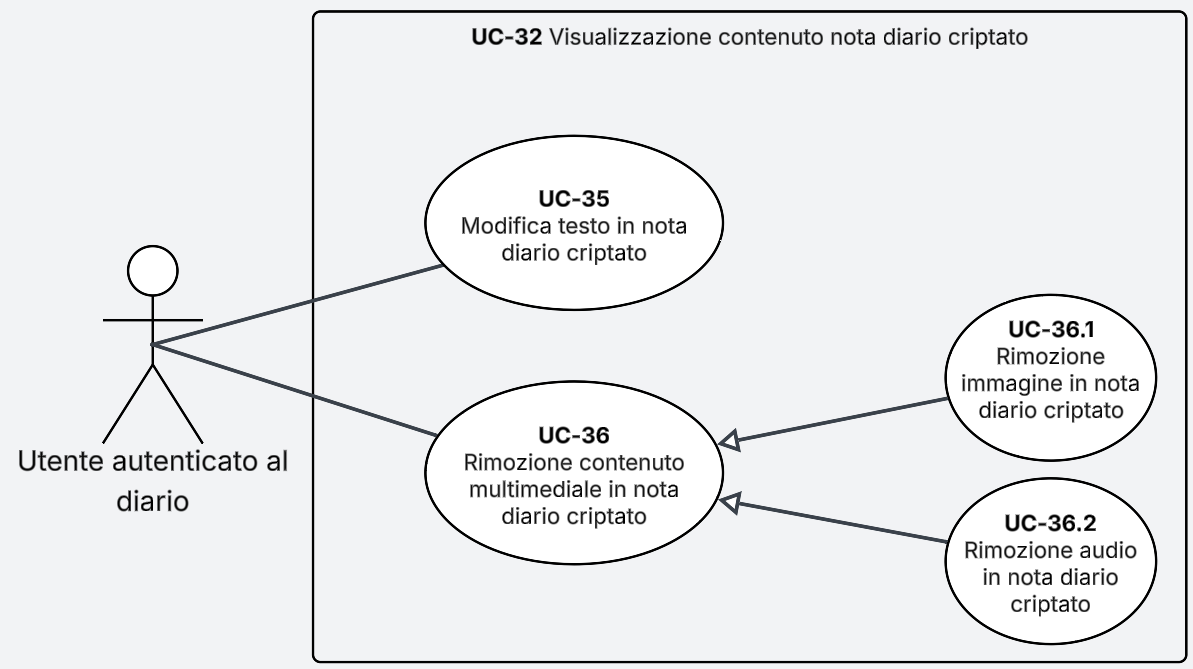
\includegraphics[width=1\textwidth]{use_case/UC-35_32-diario.png}
    \caption{Diagramma dei casi d'uso UC-35, UC-36, UC-36.1 e UC-36.2}
    \label{fig:UC-35, UC-36, UC-36.1, UC-36.2}
\end{figure}
\begin{itemize}
    \item \textbf{Attore principale:} \term{Utente} Autenticato al diario
    \item \textbf{Pre-condizioni:}
    \begin{itemize}
        \item Il sistema è attivo
        \item L'attore è all'interno del diario criptato
        \item L'attore sta visualizzando il contenuto di una nota del diario criptato
        \item È presente del contenuto testuale nella nota
    \end{itemize}
    \item \textbf{Post-condizioni:}
    \begin{itemize}
        \item L'attore ha modificato con successo il contenuto testuale nella nota
        \item Il sistema ha ricevuto correttamente la modifica del contenuto testuale ed esso è stato salvato
    \end{itemize}
    \item \textbf{Scenario principale:}
    \begin{itemize}
        \item L'attore seleziona nella nota il contenuto testuale che intende modificare
        \item L'attore modifica come desiderato il contenuto testuale selezionato
    \end{itemize}
    \item \textbf{Trigger:} L'attore vuole modificare del testo in una nota del diario criptato
\end{itemize}

\subsubsection{UC-36 - Rimozione contenuto multimediale in nota diario criptato} \label{subsec:UC-36}
\begin{itemize}
    \item \textbf{Attore principale:} \term{Utente} Autenticato al diario
    \item \textbf{Pre-condizioni:}
    \begin{itemize}
        \item Il sistema è attivo
        \item L'attore si trova all'interno del diario criptato
        \item L'attore sta visualizzando il contenuto di una nota del diario criptato
        \item La nota visualizzata contiene almeno un elemento multimediale
    \end{itemize}
    \item \textbf{Post-condizioni:}
    \begin{itemize}
        \item Il sistema riceve correttamente la rimozione del contenuto multimediale della nota
        \item Il contenuto multimediale non è più visibile nella nota
    \end{itemize}
    \item \textbf{Scenario principale:}
    \begin{itemize}
        \item L'attore seleziona il contenuto multimediale che vuole rimuovere
        \item L'attore seleziona la voce apposita per la rimozione del contenuto multimediale
        \item Il sistema rimuove definitivamente dalla nota il contenuto multimediale selezionato
    \end{itemize}
    \item \textbf{Specializzazioni}
    \begin{itemize}
        \item \hyperref[subsec:UC-36.1]{UC-36.1}
        \item \hyperref[subsec:UC-36.2]{UC-36.2}
    \end{itemize}
    \item \textbf{Trigger:} L'attore vuole rimuovere del contenuto multimediale da una nota nel diario criptato
\end{itemize}

\subsubsection{UC-36.1 - Rimozione immagine in nota diario criptato} \label{subsec:UC-36.1}
\begin{itemize}
    \item \textbf{Attore principale:} \term{Utente} Autenticato al diario
    \item \textbf{Pre-condizioni:}
    \begin{itemize}
        \item Il sistema è attivo
        \item L'attore si trova all'interno del diario criptato
        \item L'attore sta visualizzando il contenuto di una nota del diario criptato
        \item La nota visualizzata contiene almeno una immagine
    \end{itemize}
    \item \textbf{Post-condizioni:}
    \begin{itemize}
        \item Il sistema riceve correttamente la rimozione dell'immagine della nota
        \item L'immagine non è più visibile nella nota
    \end{itemize}
    \item \textbf{Scenario principale:}
    \begin{itemize}
        \item L'attore seleziona l'immagine che vuole rimuovere
        \item L'attore seleziona la voce apposita per la rimozione dell'immagine
        \item Il sistema rimuove definitivamente dalla nota l'immagine selezionata
    \end{itemize}
    \item \textbf{Trigger:} L'attore vuole rimuovere un'immagine da una nota nel diario criptato
\end{itemize}

\subsubsection{UC-36.2 - Rimozione audio in nota diario criptato} \label{subsec:UC-36.2}
\begin{itemize}
    \item \textbf{Attore principale:} \term{Utente} Autenticato al diario
    \item \textbf{Pre-condizioni:}
    \begin{itemize}
        \item Il sistema è attivo
        \item L'attore si trova all'interno del diario criptato
        \item L'attore sta visualizzando il contenuto di una nota del diario criptato
        \item La nota visualizzata contiene almeno una traccia audio
    \end{itemize}
    \item \textbf{Post-condizioni:}
    \begin{itemize}
        \item Il sistema riceve correttamente la rimozione della traccia audio della nota
        \item La traccia audio non è più presente nella nota
    \end{itemize}
    \item \textbf{Scenario principale:}
    \begin{itemize}
        \item L'attore seleziona la traccia audio che vuole rimuovere
        \item L'attore seleziona la voce apposita per la rimozione della traccia audio
        \item Il sistema rimuove definitivamente dalla nota la traccia audio selezionata
    \end{itemize}
    \item \textbf{Trigger:} L'attore vuole rimuovere una traccia audio da una nota nel diario criptato
\end{itemize}

\subsubsection{UC-29 - Visualizzazione diario fittizio} \label{subsec:UC-29}
\begin{figure}[H]
    \centering
    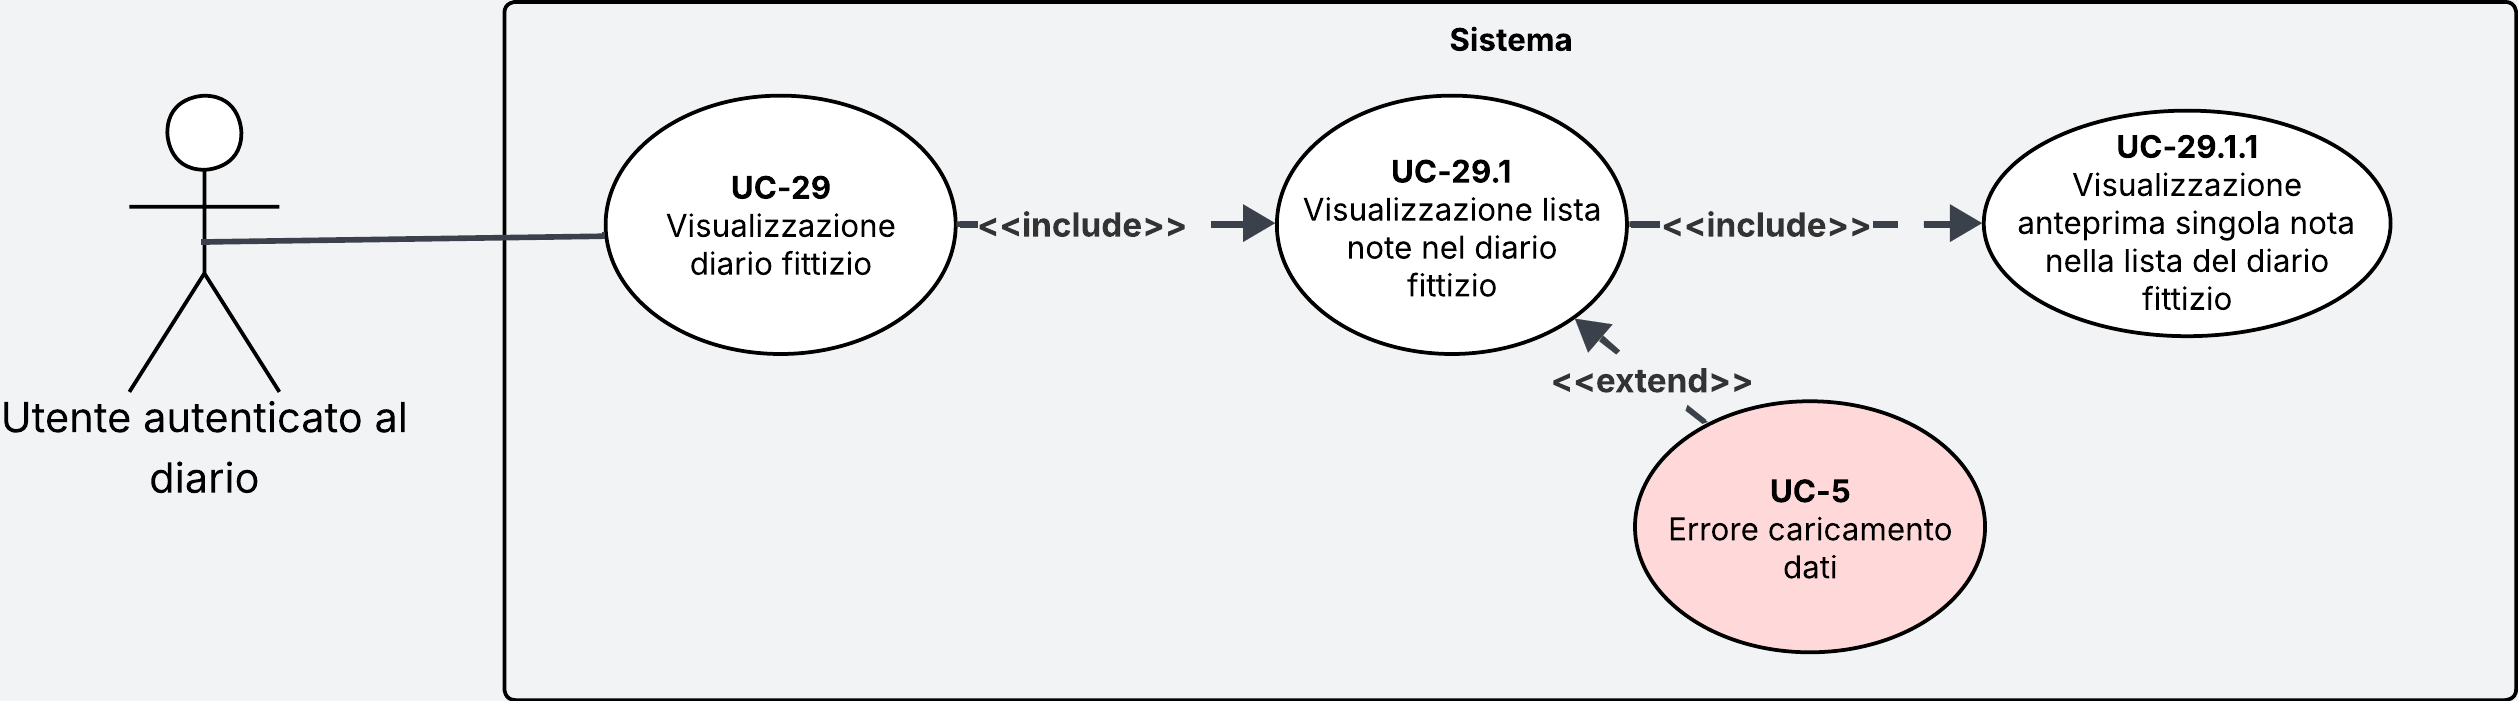
\includegraphics[width=1\textwidth]{use_case/UC-29-visualizzazione-diario-fittizio.png}
    \caption{Diagramma del caso d'uso UC-29}
    \label{fig:UC-29}
\end{figure}
\begin{itemize}
    \item \textbf{Attore principale:} \term{Utente} autenticato al diario
    \item \textbf{Pre-condizioni:}
    \begin{itemize}
        \item Il sistema è attivo
        \item L'attore si trova all'interno del diario fittizio
    \end{itemize}
    \item \textbf{Post-condizioni:} 
    \begin{itemize}
        \item Il sistema visualizza l'interfaccia principale del diario fittizio con la lista delle note
    \end{itemize}
    \item \textbf{Scenario principale:} 
    \begin{itemize}
        \item L'attore accede alla schermata principale del diario fittizio
        \item Il sistema carica e visualizza la lista delle note presenti $\rightarrow$ \hyperref[subsec:UC-29.1]{UC-29.1}
    \end{itemize}
    \item \textbf{Inclusioni:}
    \begin{itemize}
        \item \hyperref[subsec:UC-29.1]{UC-29.1}
    \end{itemize}
    \item \textbf{Trigger:} L'attore vuole accedere al diario fittizio
\end{itemize}

\subsubsection{UC-29.1 - Visualizzazione lista note nel diario fittizio} \label{subsec:UC-29.1}
\begin{itemize}
    \item \textbf{Attore principale:} \term{Utente} autenticato al diario
    \item \textbf{Pre-condizioni:}
    \begin{itemize}
        \item Il sistema è attivo
        \item L'attore si trova all'interno del diario fittizio
        \item Esiste almeno una nota all'interno del diario fittizio
    \end{itemize}
    \item \textbf{Post-condizioni:} 
    \begin{itemize}
        \item Il sistema visualizza l'elenco completo delle anteprime delle note presenti nel diario fittizio
    \end{itemize}
    \item \textbf{Scenario principale:} 
    \begin{itemize}
        \item Il sistema recupera tutte le note memorizzate nel diario fittizio
        \item Il sistema visualizza, in una lista, le anteprime di ogni singola nota $\rightarrow$ \hyperref[subsec:UC-29.1.1]{UC-29.1.1}
    \end{itemize}
    \item \textbf{Scenario secondario:} 
    \begin{itemize}
        \item Il sistema non è in grado di recuperare le note dal database $\rightarrow$ \hyperref[sec:UC-5]{UC-5}
    \end{itemize}
    \item \textbf{Inclusioni:}
    \begin{itemize}
        \item \hyperref[subsec:UC-29.1.1]{UC-29.1.1}
    \end{itemize}
    \item \textbf{Estensioni:}
    \begin{itemize}
        \item \hyperref[sec:UC-5]{UC-5}
    \end{itemize}
    \item \textbf{Trigger:} L'attore vuole accedere al diario fittizio
\end{itemize}

\subsubsection{UC-29.1.1 - Visualizzazione anteprima singola nota della lista nel diario fittizio} \label{subsec:UC-29.1.1}
\begin{itemize}
    \item \textbf{Attore principale:} \term{Utente} autenticato al diario
    \item \textbf{Pre-condizioni:}
    \begin{itemize}
        \item Il sistema è attivo
        \item L'attore si trova all'interno del diario fittizio
        \item Esiste almeno una nota all'interno del diario fittizio
        \item L'attore sta visualizzando la sezione contenente la lista delle note del diario fittizio
        \item Il sistema ha recuperato e organizzato le anteprime delle note da visualizzare
    \end{itemize}
    \item \textbf{Post-condizioni:} 
    \begin{itemize}
        \item Il sistema visualizza l'anteprima di una nota all'interno della lista
    \end{itemize}
    \item \textbf{Scenario principale:} 
    \begin{itemize}
        \item Il sistema recupera le informazioni della nota da visualizzare
        \item Il sistema visualizza parte del contenuto testuale presente all'inizio della nota
    \end{itemize}
    \item \textbf{Trigger:} L'attore vuole accedere al diario fittizio
\end{itemize}

\subsubsection{UC-37 - Eliminazione nota diario fittizio} \label{subsec:UC-37}
\begin{figure}[H]
    \centering
    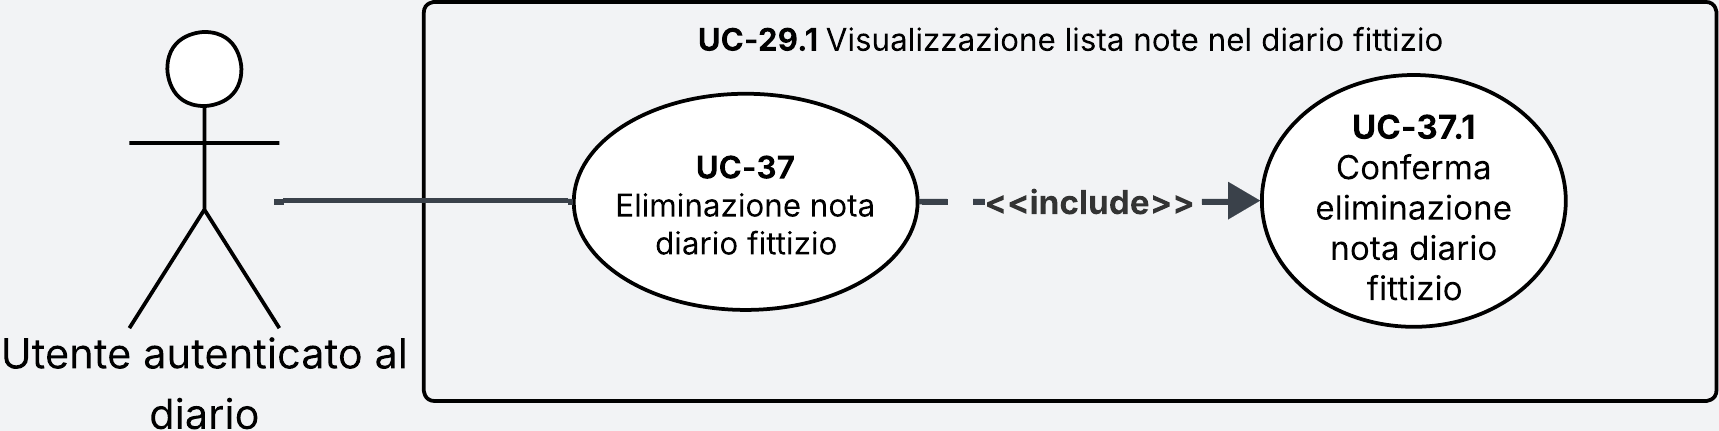
\includegraphics[width=1\textwidth]{use_case/UC-37-diario_fittizio.png}
    \caption{Diagramma dei casi d'uso UC-37 e UC-37.1}
    \label{fig:UC-37, UC-37.1}
\end{figure}
\begin{itemize}
    \item \textbf{Attore principale:} \term{Utente} Autenticato al diario
    \item \textbf{Pre-condizioni:}
    \begin{itemize}
        \item Il sistema è attivo
        \item L'attore è all'interno del diario fittizio
        \item Esiste almeno una nota nel diario fittizio
        \item L'attore sta visualizzando la lista delle note del diario fittizio
    \end{itemize}
    \item \textbf{Post-condizioni:} 
    \begin{itemize}
        \item La nota è stata rimossa dal diario fittizio
        \item La nota non è più visibile nella lista delle note del diario fittizio
    \end{itemize}
    \item \textbf{Scenario principale:} 
    \begin{itemize}
        \item L'attore seleziona la voce di eliminazione di una nota dalla lista di note del diario fittizio
        \item Il sistema richiede conferma dell'operazione di eliminazione $\rightarrow$ \hyperref[subsec:UC-37.1]{UC-37.1}
        \item L'attore conferma l'eliminazione
        \item Il sistema rimuove definitivamente la nota dal diario fittizio
        \item Il sistema aggiorna la lista delle note
    \end{itemize}
    \item \textbf{Inclusioni:}
    \begin{itemize}
        \item \hyperref[subsec:UC-37.1]{UC-37.1}
    \end{itemize}
    \item \textbf{Trigger:} L'attore vuole eliminare una nota del diario fittizio
\end{itemize}

\subsubsection{UC-37.1 - Conferma eliminazione nota diario fittizio}\label{subsec:UC-37.1}
\begin{itemize}
    \item \textbf{Attore principale:} \term{Utente} Autenticato al diario
    \item \textbf{Pre-condizioni:}
    \begin{itemize}
        \item Il sistema è attivo
        \item L'attore è all'interno del diario fittizio
        \item L'attore ha selezionato la voce per eliminare una nota dalla lista delle note del diario fittizio
    \end{itemize}
    \item \textbf{Post-condizioni:} 
    \begin{itemize}
        \item Il sistema riceve la conferma dell'attore di eliminare la nota dalla lista delle note del diario fittizio
    \end{itemize}
    \item \textbf{Scenario principale:} 
    \begin{itemize}
        \item L'attore conferma l'eliminazione di una nota dalla lista di note del diario fittizio
        \item Il sistema rimuove la nota dalla lista delle note del diario fittizio
    \end{itemize}
    \item \textbf{Trigger:} L'attore vuole confermare l'eliminazione di una nota dal diario fittizio
\end{itemize}

\subsubsection{UC-38 - Creazione nota diario fittizio} \label{subsec:UC-38}
\begin{figure}[H]
    \centering
    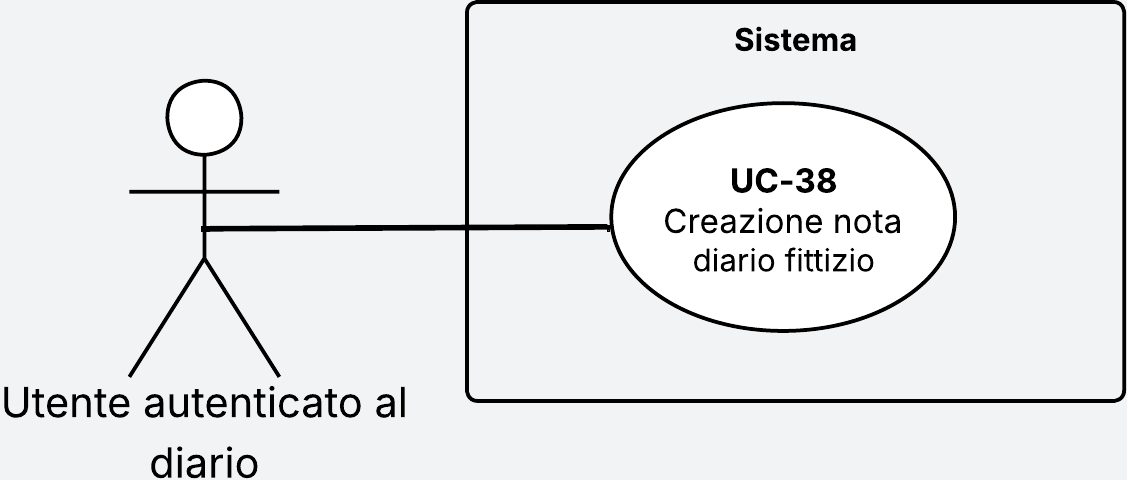
\includegraphics[width=1\textwidth]{use_case/UC-38-diario_fittizio.png}
    \caption{Diagramma del caso d'uso UC-38}
    \label{fig:UC-38}
\end{figure}
\begin{itemize}
    \item \textbf{Attore principale:} \term{Utente} Autenticato al diario
    \item \textbf{Pre-condizioni:}
    \begin{itemize}
        \item Il sistema è attivo
        \item L'attore si trova all'interno del diario fittizio
        \item L'attore sta visualizzando la lista delle note del diario fittizio
    \end{itemize}
    \item \textbf{Post-condizioni:} 
    \begin{itemize}
        \item Il sistema crea una nuova nota vuota e la memorizza nel diario fittizio
    \end{itemize}
    \item \textbf{Scenario principale:} 
    \begin{itemize}
        \item L'attore ha selezionato la voce per l'aggiunta di una nuova nota
        \item La nuova nota viene creata ed è visibile nella lista delle note del diario fittizio
    \end{itemize}
    \item \textbf{Trigger:} L'attore vuole creare una nuova nota nel diario fittizio
\end{itemize}

\subsubsection{UC-39 - Visualizzazione contenuto nota diario fittizio} \label{subsec:UC-39}
\begin{figure}[H]
    \centering
    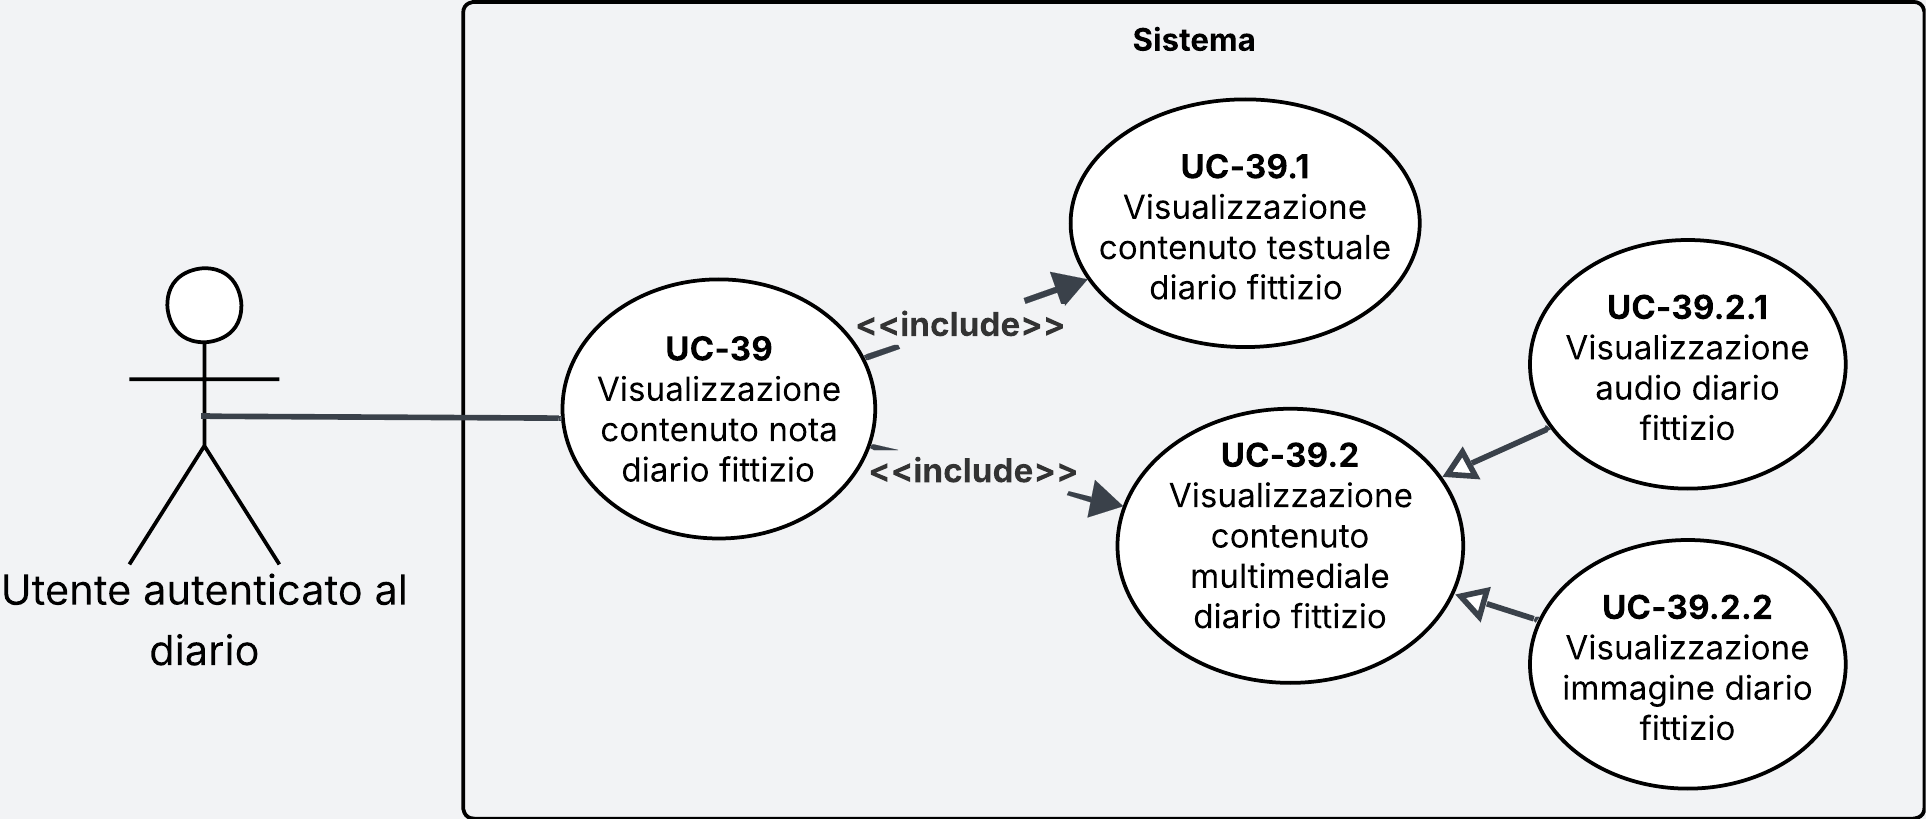
\includegraphics[width=1\textwidth]{use_case/UC-39-diario_fittizio.png}
    \caption{Diagramma del caso d'uso UC-39}
    \label{fig:UC-39}
\end{figure}
\begin{itemize}
    \item \textbf{Attore principale:} \term{Utente} Autenticato al diario
    \item \textbf{Pre-condizioni:}
    \begin{itemize}
        \item Il sistema è attivo
        \item L'attore si trova all'interno del diario fittizio
        \item Esiste almeno una nota nel diario fittizio
        \item L'attore sta visualizzando la lista delle note nel diario fittizio
    \end{itemize}
    \item \textbf{Post-condizioni:} 
    \begin{itemize}
        \item L'attore visualizza il contenuto di una nota del diario fittizio
    \end{itemize}
    \item \textbf{Scenario principale:} 
    \begin{itemize}
        \item L'attore seleziona una nota dalla lista
        \item Il sistema recupera il contenuto completo della nota
        \item Il sistema visualizza a schermo il contenuto testuale della nota $\rightarrow$ \hyperref[subsec:UC-39.1]{UC-39.1}
        \item Il sistema visualizza a schermo il contenuto multimediale della nota $\rightarrow$ \hyperref[subsec:UC-39.2]{UC-39.2}
        \item L'attore può visualizzare e interagire con il contenuto della nota
    \end{itemize}
    \item \textbf{Inclusioni:}
    \begin{itemize}
        \item \hyperref[subsec:UC-39.1]{UC-39.1}
        \item \hyperref[subsec:UC-39.2]{UC-39.2}
    \end{itemize}
    \item \textbf{Trigger:} L'attore vuole visualizzare il contenuto di una nota nel diario fittizio
\end{itemize}

\subsubsection{UC-39.1 - Visualizzazione contenuto testuale nota diario fittizio} \label{subsec:UC-39.1}
\begin{itemize}
    \item \textbf{Attore principale:} \term{Utente} Autenticato al diario
    \item \textbf{Pre-condizioni:}
    \begin{itemize}
        \item Il sistema è attivo
        \item L'attore si trova all'interno del diario fittizio
        \item Esiste almeno una nota nel diario fittizio
        \item L'attore sta visualizzando il contenuto di una nota del diario fittizio
    \end{itemize}
    \item \textbf{Post-condizioni:}
    \begin{itemize}
        \item L'attore visualizza il contenuto testuale della nota
    \end{itemize}
    \item \textbf{Scenario principale:}
    \begin{itemize}
        \item Il sistema mostra il contenuto testuale della nota 
    \end{itemize}
    \item \textbf{Trigger:} L'attore vuole visualizzare il contenuto testuale di una nota del diario fittizio
\end{itemize}

\subsubsection{UC-39.2 - Visualizzazione contenuto multimediale nota diario fittizio} \label{subsec:UC-39.2}
\begin{itemize}
    \item \textbf{Attore principale:} \term{Utente} Autenticato al diario
    \item \textbf{Pre-condizioni:}
    \begin{itemize}
        \item Il sistema è attivo
        \item L'attore si trova all'interno del diario fittizio
        \item Esiste almeno una nota nel diario fittizio
        \item L'attore sta visualizzando il contenuto di una nota del diario fittizio
    \end{itemize}
    \item \textbf{Post-condizioni:}
    \begin{itemize}
        \item L'attore visualizza il contenuto multimediale della nota
    \end{itemize}
    \item \textbf{Scenario principale:}
    \begin{itemize}
        \item Il sistema mostra il contenuto multimediale della nota 
    \end{itemize}
    \item \textbf{Specializzazioni:}
    \begin{itemize}
        \item \hyperref[subsec:UC-39.2.1]{UC-39.2.1}
        \item \hyperref[subsec:UC-39.2.2]{UC-39.2.2}
    \end{itemize}
    \item \textbf{Trigger:} L'attore vuole visualizzare il contenuto multimediale di una nota del diario fittizio
\end{itemize}

\subsubsection{UC-39.2.1 - Visualizzazione audio nota diario fittizio} \label{subsec:UC-39.2.1}
\begin{itemize}
    \item \textbf{Attore principale:} \term{Utente} Autenticato al diario
    \item \textbf{Pre-condizioni:}
    \begin{itemize}
        \item Il sistema è attivo
        \item L'attore si trova all'interno del diario fittizio
        \item Esiste almeno una nota nel diario fittizio
        \item L'attore sta visualizzando il contenuto di una nota del diario fittizio
    \end{itemize}
    \item \textbf{Post-condizioni:}
    \begin{itemize}
        \item L'attore visualizza il contenuto audio presente nella nota
    \end{itemize}
    \item \textbf{Scenario principale:}
    \begin{itemize}
        \item Il sistema mostra il contenuto audio presente nella nota 
    \end{itemize}
    \item \textbf{Trigger:} L'attore vuole visualizzare il contenuto audio di una nota del diario fittizio
\end{itemize}

\subsubsection{UC-39.2.2 - Visualizzazione immagini nota diario fittizio} \label{subsec:UC-39.2.2}
\begin{itemize}
    \item \textbf{Attore principale:} \term{Utente} Autenticato al diario
    \item \textbf{Pre-condizioni:}
    \begin{itemize}
        \item Il sistema è attivo
        \item L'attore si trova all'interno del diario fittizio
        \item Esiste almeno una nota nel diario fittizio
        \item L'attore sta visualizzando il contenuto di una nota del diario fittizio
    \end{itemize}
    \item \textbf{Post-condizioni:}
    \begin{itemize}
        \item L'attore visualizza le immagini presenti nella nota
    \end{itemize}
    \item \textbf{Scenario principale:}
    \begin{itemize}
        \item Il sistema mostra le immagini presenti nella nota 
    \end{itemize}
    \item \textbf{Trigger:} L'attore vuole visualizzare le immagini contenute in una nota del diario fittizio
\end{itemize}

\subsubsection{UC-40 - Inserimento testo in nota diario fittizio} \label{subsec:UC-40}
\begin{figure}[H]
    \centering
    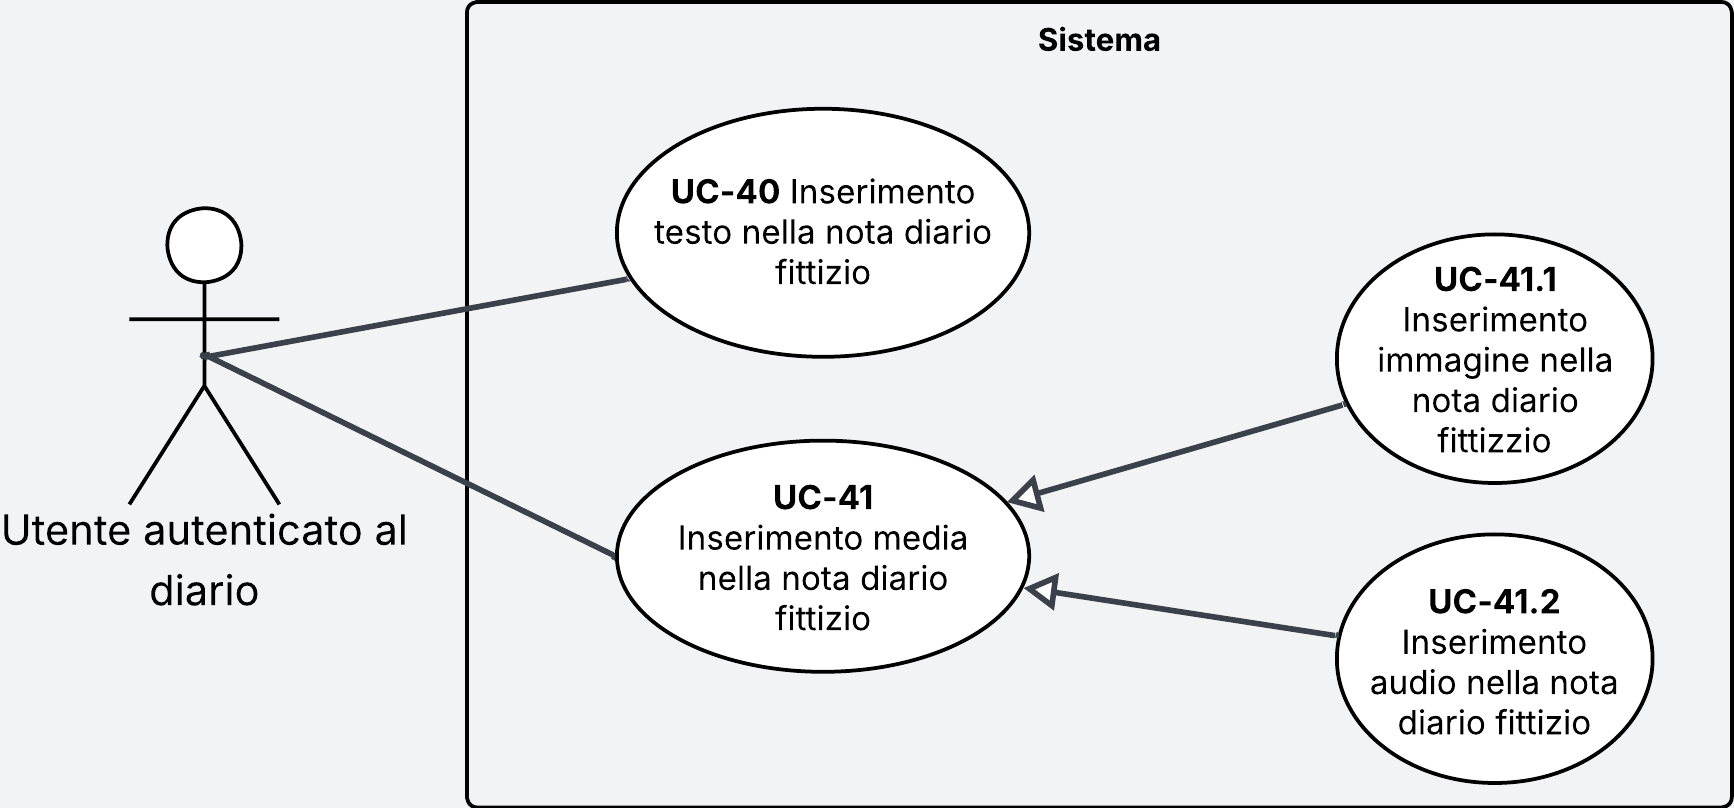
\includegraphics[width=1\textwidth]{use_case/UC-40-41-diario_fittizio.png}
    \caption{Diagramma dei casi d'uso UC-40, UC-41, UC-41.1 e UC-41.2}
    \label{fig:UC-40, UC-341, UC-41.1, UC-41.2}
\end{figure}
\begin{itemize}
    \item \textbf{Attore principale:} \term{Utente} Autenticato al diario
    \item \textbf{Pre-condizioni:}
    \begin{itemize}
        \item Il sistema è attivo
        \item L'attore si trova all'interno del diario fittizio
        \item L'attore sta visualizzando il contenuto di una nota del diario fittizio
        \item Non è presente contenuto testuale nella nota
    \end{itemize}
    \item \textbf{Post-condizioni:}
    \begin{itemize}
        \item Il sistema riceve correttamente il testo digitato da memorizzare nella nota
    \end{itemize}
    \item \textbf{Scenario principale:}
    \begin{itemize}
        \item L'attore ha selezionato l'area apposita per l'inserimento del testo nella nota
        \item L'attore digita il testo da inserire nella nota
    \end{itemize}
    \item \textbf{Trigger:} L'attore vuole aggiungere del testo ad una nota nel diario fittizio
\end{itemize}

\subsubsection{UC-41 - Inserimento media in nota diario fittizio} \label{subsec:UC-41}
\begin{itemize}
    \item \textbf{Attore principale:} \term{Utente} Autenticato al diario
    \item \textbf{Pre-condizioni:}
    \begin{itemize}
        \item Il sistema è attivo
        \item L'attore si trova all'interno del diario fittizio
        \item L'attore sta visualizzando il contenuto di una nota del diario fittizio
    \end{itemize}
    \item \textbf{Post-condizioni:}
    \begin{itemize}
        \item Il sistema riceve correttamente il media da memorizzare nella nota
    \end{itemize}
    \item \textbf{Scenario principale:}
    \begin{itemize}
        \item L'attore ha selezionato la voce per l'aggiunta di un media
        \item L'attore inserisce il media desiderato
    \end{itemize}
    \item \textbf{Specializzazioni}
    \begin{itemize}
        \item \hyperref[subsec:UC-41.1]{UC-41.1}
        \item \hyperref[subsec:UC-41.2]{UC-41.2}
    \end{itemize}
    \item \textbf{Trigger:} L'attore vuole aggiungere del contenuto multimediale ad una nota nel diario fittizio
\end{itemize}

\subsubsection{UC-41.1 - Inserimento immagine nella nota diario fittizio} \label{subsec:UC-41.1}
\begin{itemize}
    \item \textbf{Attore principale:} \term{Utente} Autenticato al diario
    \item \textbf{Pre-condizioni:}
    \begin{itemize}
        \item Il sistema è attivo
        \item L'attore si trova all'interno del diario fittizio
        \item L'attore sta visualizzando il contenuto di una nota del diario fittizio
    \end{itemize}
    \item \textbf{Post-condizioni:}
    \begin{itemize}
        \item Il sistema riceve correttamente l'immagine da memorizzare nella nota
    \end{itemize}
    \item \textbf{Scenario principale:}
    \begin{itemize}
        \item L'attore ha selezionato la voce per l'aggiunta di un media
        \item L'attore inserisce una immagine nella nota
    \end{itemize}
    \item \textbf{Trigger:} L'attore vuole aggiungere un'immagine ad una nota nel diario fittizio
\end{itemize}

\subsubsection{UC-41.2 - Inserimento audio nella nota diario fittizio} \label{subsec:UC-41.2}
\begin{itemize}
    \item \textbf{Attore principale:} \term{Utente} Autenticato al diario
    \item \textbf{Pre-condizioni:}
    \begin{itemize}
        \item Il sistema è attivo
        \item L'attore si trova all'interno del diario fittizio
        \item L'attore sta visualizzando il contenuto di una nota del diario fittizio
    \end{itemize}
    \item \textbf{Post-condizioni:}
    \begin{itemize}
        \item Il sistema riceve correttamente l'audio da memorizzare nella nota
    \end{itemize}
    \item \textbf{Scenario principale:}
    \begin{itemize}
        \item L'attore ha selezionato la voce per l'aggiunta di un media
        \item L'attore inserisce un audio nella nota
    \end{itemize}
    \item \textbf{Trigger:} L'attore vuole aggiungere del contenuto audio ad una nota nel diario fittizio
\end{itemize}

\subsubsection{UC-42 - Rimozione contenuto multimediale in nota diario fittizio} \label{subsec:UC-42}
\begin{figure}[H]
    \centering
    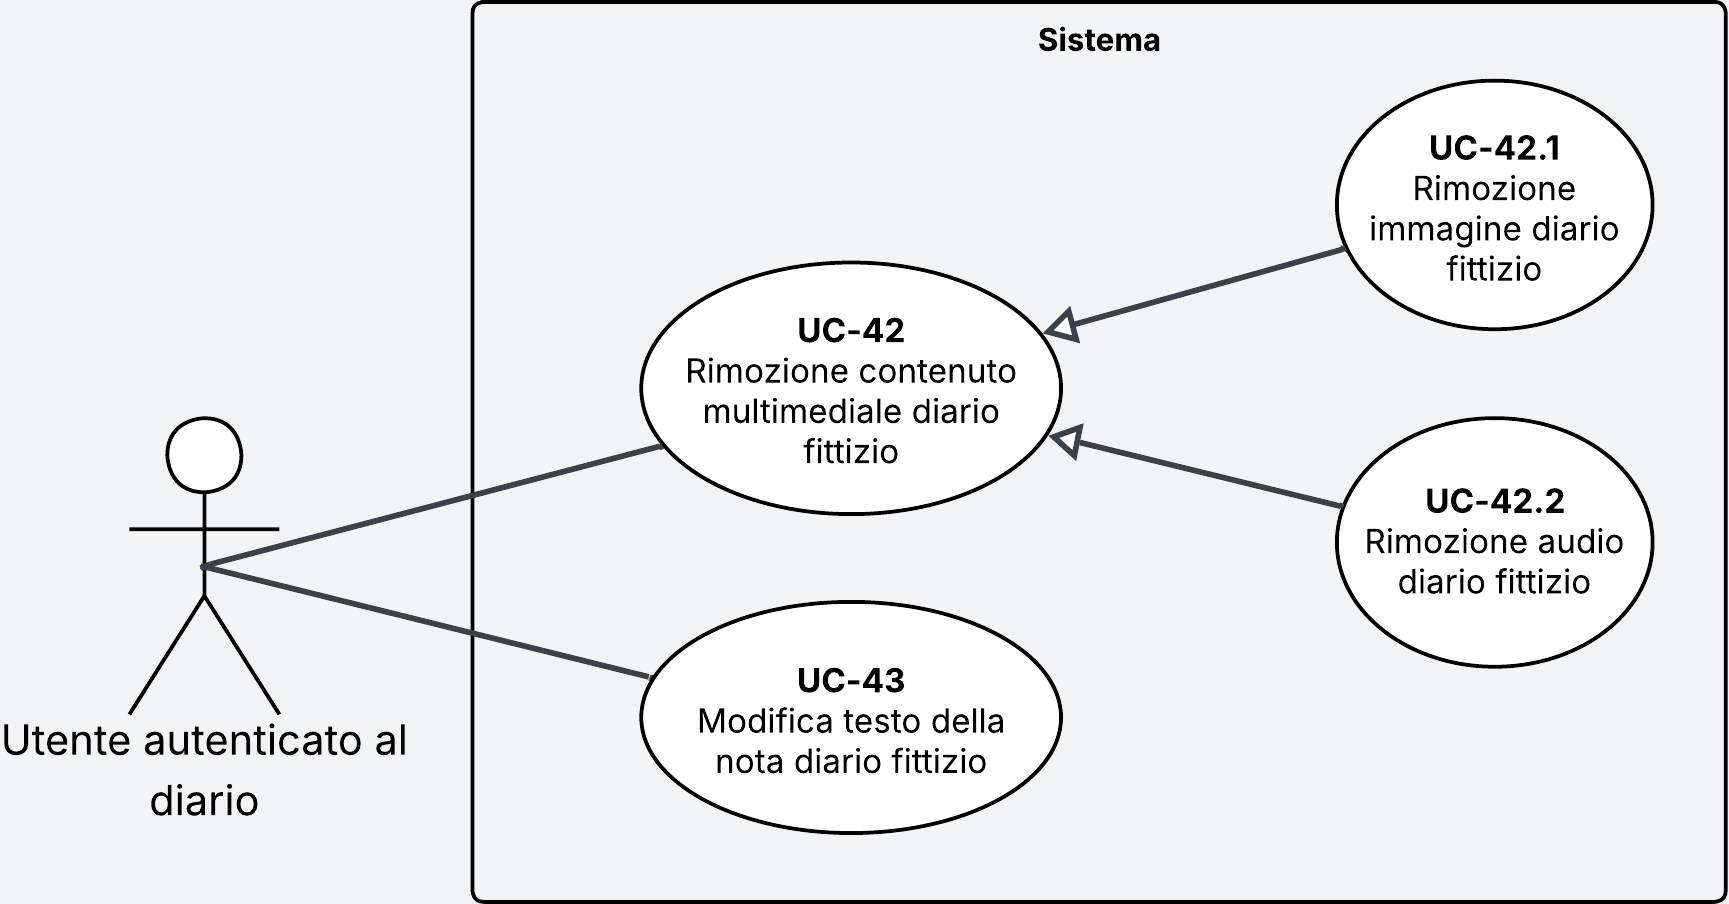
\includegraphics[width=1\textwidth]{use_case/UC-42-43-diario_fittizio.png}
    \caption{Diagramma dei casi d'uso UC-42, UC-43, UC-42.1 e UC-42.2}
    \label{fig:UC-42, UC-43, UC-42.1, UC-42.2}
\end{figure}
\begin{itemize}
    \item \textbf{Attore principale:} \term{Utente} Autenticato al diario
    \item \textbf{Pre-condizioni:}
    \begin{itemize}
        \item Il sistema è attivo
        \item L'attore si trova all'interno del diario fittizio
        \item L'attore sta visualizzando il contenuto di una nota del diario fittizio
        \item La nota visualizzata contiene almeno un elemento multimediale
    \end{itemize}
    \item \textbf{Post-condizioni:}
    \begin{itemize}
        \item Il sistema riceve correttamente la rimozione del contenuto multimediale della nota
        \item Il contenuto multimediale non è più visibile nella nota
    \end{itemize}
    \item \textbf{Scenario principale:}
    \begin{itemize}
        \item L'attore seleziona il contenuto multimediale che vuole rimuovere
        \item L'attore seleziona la voce apposita per la rimozione del contenuto multimediale
        \item Il sistema rimuove il contenuto multimediale definitivamente dalla nota
    \end{itemize}
    \item \textbf{Specializzazioni}
    \begin{itemize}
        \item \hyperref[subsec:UC-42.1]{UC-42.1}
        \item \hyperref[subsec:UC-42.2]{UC-42.2}
    \end{itemize}
    \item \textbf{Trigger:} L'attore vuole rimuovere del contenuto multimediale da una nota nel diario fittizio
\end{itemize}

\subsubsection{UC-42.1 - Rimozione immagine in nota diario fittizio} \label{subsec:UC-42.1}
\begin{itemize}
    \item \textbf{Attore principale:} \term{Utente} Autenticato al diario
    \item \textbf{Pre-condizioni:}
    \begin{itemize}
        \item Il sistema è attivo
        \item L'attore si trova all'interno del diario fittizio
        \item L'attore sta visualizzando il contenuto di una nota del diario fittizio
        \item La nota visualizzata contiene almeno una immagine
    \end{itemize}
    \item \textbf{Post-condizioni:}
    \begin{itemize}
        \item Il sistema riceve correttamente la rimozione dell'immagine della nota
        \item L'immagine non è più visibile nella nota
    \end{itemize}
    \item \textbf{Scenario principale:}
    \begin{itemize}
        \item L'attore seleziona l'immagine che vuole rimuovere
        \item L'attore seleziona la voce apposita per la rimozione dell'immagine
        \item Il sistema rimuove l'immagine definitivamente dalla nota
    \end{itemize}
    \item \textbf{Trigger:} L'attore vuole rimuovere un'immagine da una nota nel diario fittizio
\end{itemize}

\subsubsection{UC-42.2 - Rimozione audio in nota diario fittizio} \label{subsec:UC-42.2}
\begin{itemize}
    \item \textbf{Attore principale:} \term{Utente} Autenticato al diario
    \item \textbf{Pre-condizioni:}
    \begin{itemize}
        \item Il sistema è attivo
        \item L'attore si trova all'interno del diario fittizio
        \item L'attore sta visualizzando il contenuto di una nota del diario fittizio
        \item La nota visualizzata contiene almeno una traccia audio
    \end{itemize}
    \item \textbf{Post-condizioni:}
    \begin{itemize}
        \item Il sistema riceve correttamente la rimozione della traccia audio della nota
        \item La traccia audio non è più presente nella nota
    \end{itemize}
    \item \textbf{Scenario principale:}
    \begin{itemize}
        \item L'attore seleziona la traccia audio che vuole rimuovere
        \item L'attore seleziona la voce apposita per la rimozione della traccia audio
        \item Il sistema rimuove la traccia audio definitivamente dalla nota
    \end{itemize}
    \item \textbf{Trigger:} L'attore vuole rimuovere una traccia audio da una nota nel diario fittizio
\end{itemize}

\subsubsection{UC-43 - Modifica testo in nota diario fittizio} \label{subsec:UC-43}
\begin{itemize}
    \item \textbf{Attore principale:} \term{Utente} Autenticato al diario
    \item \textbf{Pre-condizioni:}
    \begin{itemize}
        \item Il sistema è attivo
        \item L'attore è all'interno del diario fittizio
        \item L'attore sta visualizzando il contenuto di una nota del diario fittizio
        \item È presente del contenuto testuale nella nota
    \end{itemize}
    \item \textbf{Post-condizioni:}
    \begin{itemize}
        \item L'attore ha modificato con successo il contenuto testuale nella nota
        \item Il sistema ha ricevuto correttamente la modifica del contenuto testuale ed esso è stato salvato
    \end{itemize}
    \item \textbf{Scenario principale:}
    \begin{itemize}
        \item L'attore seleziona nella nota il contenuto testuale che intende modificare
        \item L'attore modifica come desiderato il contenuto testuale selezionato
    \end{itemize}
    \item \textbf{Trigger:} L'attore vuole modificare del testo in una nota del diario fittizio
\end{itemize}


% ===== UC-S: SICUREZZA - GUARDIANO SILENZIOSO  ======

\subsubsection{UC-44 - Invio messaggio SOS} \label{sec:UC-44}

\begin{figure}[H]
    \centering
    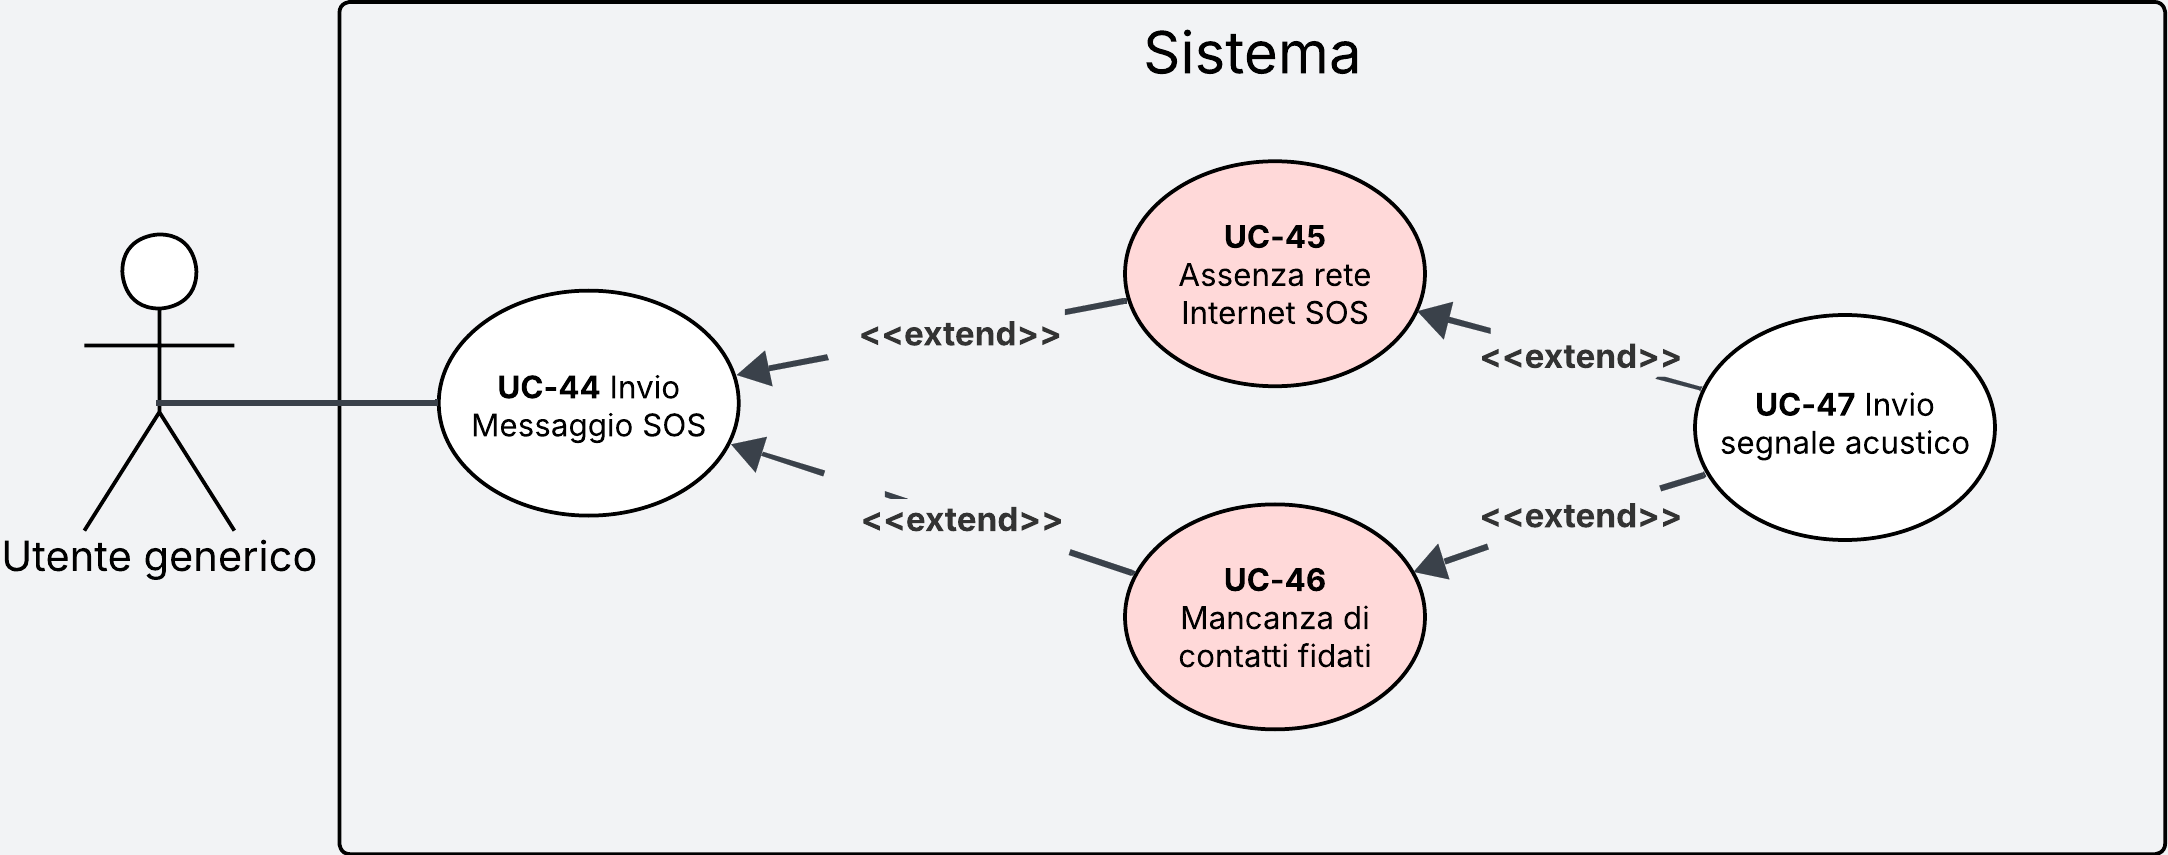
\includegraphics[width=1\textwidth]{use_case/UC-44-47-guardiano.png}
    \caption{Diagramma del caso d'uso UC-44}
    \label{fig:UC-44}
\end{figure}

\begin{itemize}
    \item \textbf{Attore principale:} \term{Utente} Generico
    \item \textbf{Pre-condizioni:} 
    \begin{itemize}
        \item Il sistema è attivo.
        \item L'attore ha cliccato la voce per l'invio del messaggio SOS.
    \end{itemize}
    \item \textbf{Post-condizioni:}
    \begin{itemize}
        \item Il sistema ha inviato il messaggio di SOS ai contatti fidati dell'attore.
    \end{itemize}
    \item \textbf{Scenario principale:} 
    \begin{itemize}
        \item L’attore interagisce con l'opzione di invio del messaggio SOS.
        \item Il sistema \ignoreglossary{verifica} la presenza di connessione.
	    \item Il sistema invia una mail preimpostata ai contatti fidati memorizzati.
    \end{itemize}
    \item \textbf{Scenari secondari:} 
    \begin{itemize}
        \item Il sistema non è in grado di connettersi a internet. $\rightarrow$ \hyperref[sec:UC-45]{UC-45}
        \item L'attore non ha inserito nessun contatto fidato nella rete dei contatti fidati. $\rightarrow$ \hyperref[sec:UC-46]{UC-46}
    \end{itemize}
    \item \textbf{Estensioni:}
    \begin{itemize}
        \item \hyperref[sec:UC-45]{UC-45}
        \item \hyperref[sec:UC-46]{UC-46}
    \end{itemize}
    \item \textbf{Trigger:} L'attore interagisce con l'opzione di invio del messaggio SOS.
\end{itemize}

\subsubsection{UC-45 - Assenza rete Internet SOS} \label{sec:UC-45}
\begin{itemize}
    \item \textbf{Attore principale:} \term{Utente} Generico
    \item \textbf{Pre-condizioni:} 
    \begin{itemize}
        \item Il sistema è attivo.
	    \item L'attore ha richiesto l'invio del messaggio di SOS.
	    \item Il sistema non ha accesso alla connessione internet.
    \end{itemize}	

    \item \textbf{Post-condizioni:}
    \begin{itemize}
        \item Il sistema ha notificato l'attore dell'errore
        \item Il sistema ha proposto all'attore l'opzione di invio del segnale acustico.
    \end{itemize}
    \item \textbf{Scenario principale:} 
    \begin{itemize}
        \item Il sistema ha rilevato l'assenza di connessione.
        \item Il sistema mostra un messaggio di errore.
        \item Il sistema dà la possibilità all'attore di inviare un segnale acustico $\rightarrow$ \hyperref[sec:UC-47]{UC-47}
    \end{itemize}
    \item \textbf{Estensioni:}
    \begin{itemize}
        \item \hyperref[sec:UC-47]{UC-47}
    \end{itemize}
    \item \textbf{Trigger:} L'attore ha cliccato l'elemento per inviare un messaggio di SOS ma il sistema rileva l'assenza di connessione internet.
\end{itemize}

\subsubsection{UC-46 - Mancanza di contatti fidati} \label{sec:UC-46}
\begin{itemize}
    \item \textbf{Attore principale:} \term{Utente} Generico
    \item \textbf{Pre-condizioni:}
    \begin{itemize}
        \item Il sistema è attivo.
	    \item L'attore ha richiesto l'invio del messaggio di SOS.
	    \item La lista dei contatti fidati è vuota.
    \end{itemize}	
    \item \textbf{Post-condizioni:} 
    \begin{itemize}
        \item Il sistema ha notificato l'attore dell'errore
        \item Il sistema ha proposto all'attore l'opzione di invio del segnale acustico.
    \end{itemize}
    \item \textbf{Scenario principale:} 
    \begin{itemize}
        \item Il sistema rileva che la lista dei contatti fidati è vuota
        \item Il sistema notifica l'attore con un messaggio di errore
        \item Il sistema dà la possibilità all'attore di inviare un segnale acustico $\rightarrow$  \hyperref[sec:UC-47]{UC-47}
    \end{itemize}
    \item \textbf{Estensioni:}
    \begin{itemize}
        \item  \hyperref[sec:UC-47]{UC-47}
    \end{itemize}
    \item \textbf{Trigger:} L'attore vuole mandare un messaggio di SOS ai contatti fidati
\end{itemize}

\subsubsection{UC-47 - Invio segnale acustico} \label{sec:UC-47}
\begin{itemize}
    \item \textbf{Attore principale:} \term{Utente} Generico
    \item \textbf{Pre-condizioni:}
    \begin{itemize}
        \item Il sistema è attivo.
	    \item L'attore ha richiesto l'invio del messaggio di SOS.
	    \item Si è verificato un errore che ha impedito l'invio delle mail ai contatti fidati.
        \item L'attore ha selezionato l'opzione di invio del segnale acustico.
    \end{itemize}	
    \item \textbf{Post-condizioni:} 
    \begin{itemize}
        \item Il sistema avvia l'invio di un segnale acustico
    \end{itemize}
    \item \textbf{Scenario principale:} 
    \begin{itemize}
        \item L'attore seleziona l'opzione per inviare il segnale acustico.
        \item Il sistema invia il segnale acustico indipendente dalle impostazioni di volume del dispositivo.
    \end{itemize}
    \item \textbf{Trigger:} L'attore vuole avviare il segnale acustico data l'impossibilità di inviare il messaggio di SOS.
\end{itemize}

% ========================== UC-I: I - DETECTIVE DELLE RELAZIONI  ==============================


\subsubsection{UC-48 - Consultazione chatbot} \label{sec:UC-48}

\begin{figure}[H]
    \centering
    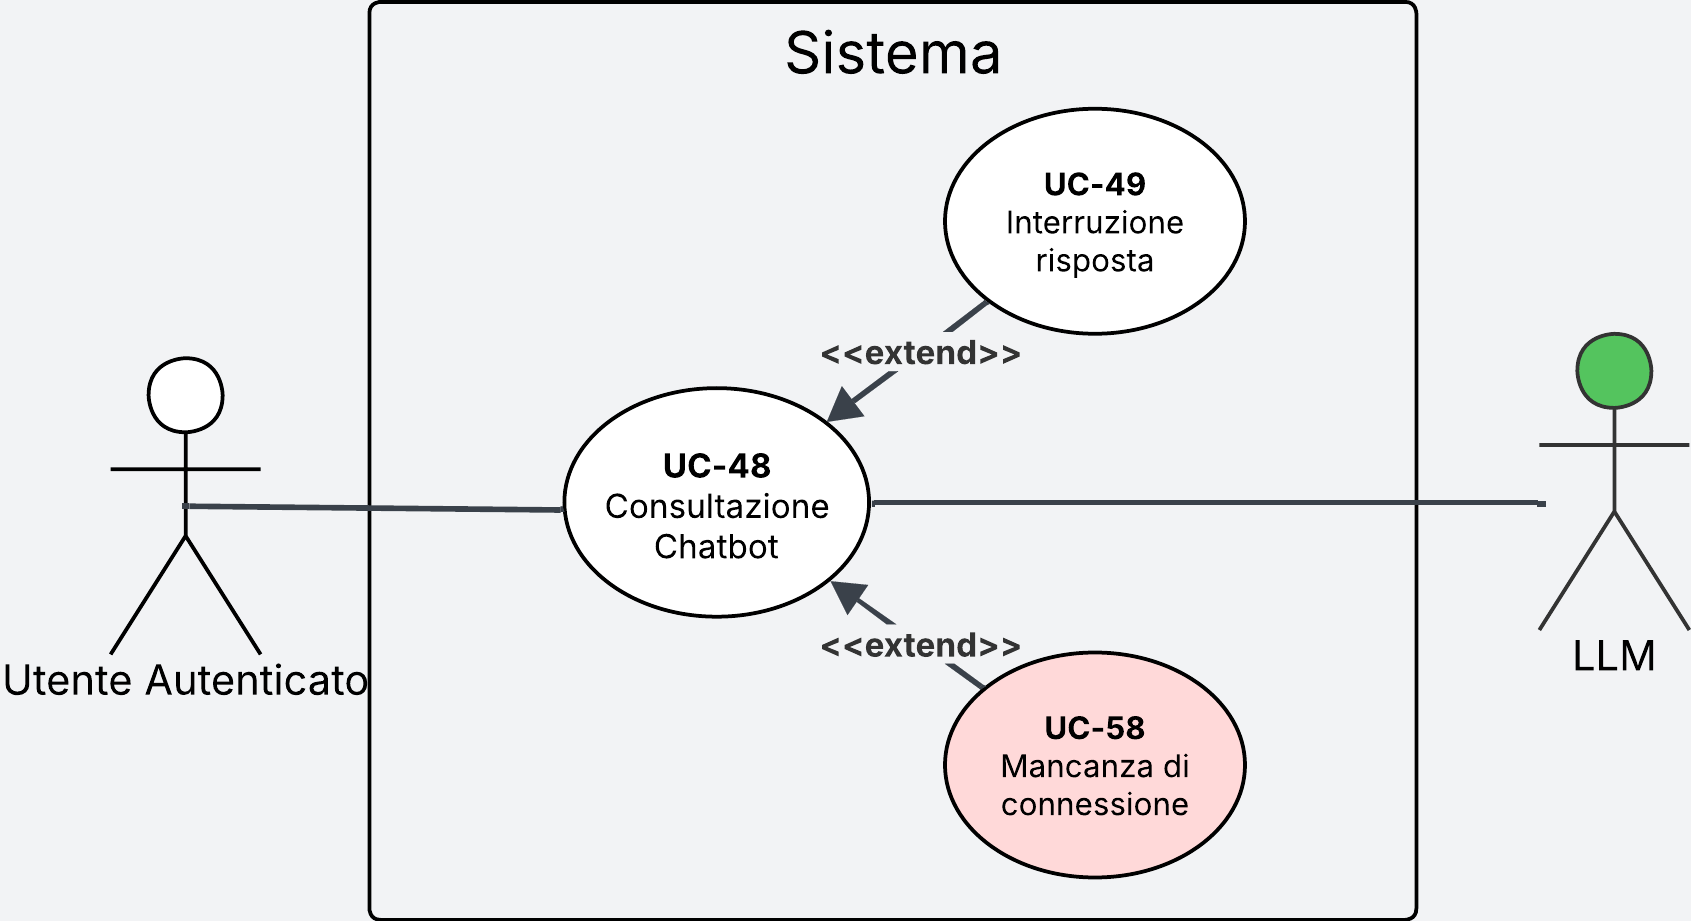
\includegraphics[width=1\textwidth]{use_case/UC-48-detective.png}
    \caption{Diagramma del caso d'uso UC-48}
    \label{fig:UC-48}
\end{figure}

\begin{itemize}
    \item \textbf{Attore principale:} \term{Utente} Autenticato
    \item \textbf{Attore secondario:} LLM
    \item \textbf{Pre-condizioni:}
    \begin{itemize}
        \item Il sistema è attivo
        \item L'attore sta visualizzando una chat
    \end{itemize}
    \item \textbf{Post-condizioni:}
    \begin{itemize}
        \item L'attore ha ricevuto una risposta dall'LLM
    \end{itemize}
    \item \textbf{Scenario principale:} 
    \begin{itemize}
        \item L'attore inserisce il messaggio nella sezione apposita
        \item L'attore invia il messaggio al chatbot impostato nel contesto scelto
        \item Il chatbot analizza il messaggio secondo i prompt impostati dal contesto
        \item Il chatbot analizza il messaggio secondo la cronologia dei messaggi
        \item Il chatbot genera la risposta
        \item L'attore visualizza la risposta del chatbot a schermo
    \end{itemize}
    \item \textbf{Scenario secondario:} 
    \begin{itemize}
        \item L'attore interrompe il \ignoreglossary{processo} di analisi del messaggio dell'LLM \hyperref[sec:UC-49]{UC-49}
        \item Il messaggio non riesce ad essere inviato causa mancanza di connessione \hyperref[sec:UC-50]{UC-50}
    \end{itemize}
    \item \textbf{Estensioni:}
    \begin{itemize}
        \item \hyperref[sec:UC-49]{UC-49}
        \item \hyperref[sec:UC-50]{UC-50}
    \end{itemize}
    \item \textbf{Trigger:} L'attore vuole consultarsi con il chatbot
\end{itemize}

\subsubsection{UC-49 - Interruzione risposta} \label{sec:UC-49}
\begin{itemize}
    \item \textbf{Attore principale:} \term{Utente} Autenticato
    \item \textbf{Pre-condizioni:} 
    \begin{itemize}
        \item Il sistema è attivo
	    \item L'attore ha mandato un messaggio
	    \item Il sistema ha ricevuto il messaggio
    \end{itemize}	
    \item \textbf{Post-condizioni:}
    \begin{itemize}
        \item Il sistema ha interrotto la generazione della risposta
    \end{itemize}
    \item \textbf{Scenario principale:} 
    \begin{itemize}
        \item L'attore interrompe l'LLM durante l'analisi del messaggio
        \item Il sistema smette di analizzare il messaggio
        \item Il sistema notifica l'attore dell'interruzione della generazione della risposta
        \item L'attore può riscrivere un messaggio al chatbot
    \end{itemize}
    \item \textbf{Trigger:} L'attore vuole interrompere la generazione della risposta dell'LLM
\end{itemize}

\subsubsection{UC-50 - Mancanza di connessione} \label{sec:UC-50}
\begin{itemize}
    \item \textbf{Attore principale:} \term{Utente} Autenticato
    \item \textbf{Pre-condizioni:}
    \begin{itemize}
        \item Il sistema è attivo
        \item L'attore ha inviato un messaggio al chatbot
        \item Il sistema rileva la mancanza di connessione
    \end{itemize}
    \item \textbf{Post-condizioni:}
    \begin{itemize}
        \item L'attore è notificato dell'errore
    \end{itemize}
    \item \textbf{Scenario principale:} 
    \begin{itemize}
        \item Il sistema ha rilevato che non c'è connessione
        \item Il sistema notifica l'attore della mancanza di connessione
        \item L'attore può ripetere l'invio del messaggio o scriverne uno nuovo
       \end{itemize}
    \item \textbf{Trigger:} L'attore vuole consultarsi con il chatbot ma manca la connessione internet.
\end{itemize}

\subsubsection{UC-51 - Switch al "Detective delle Relazioni"} \label{sec:UC-51}
\begin{figure}[H]
    \centering
    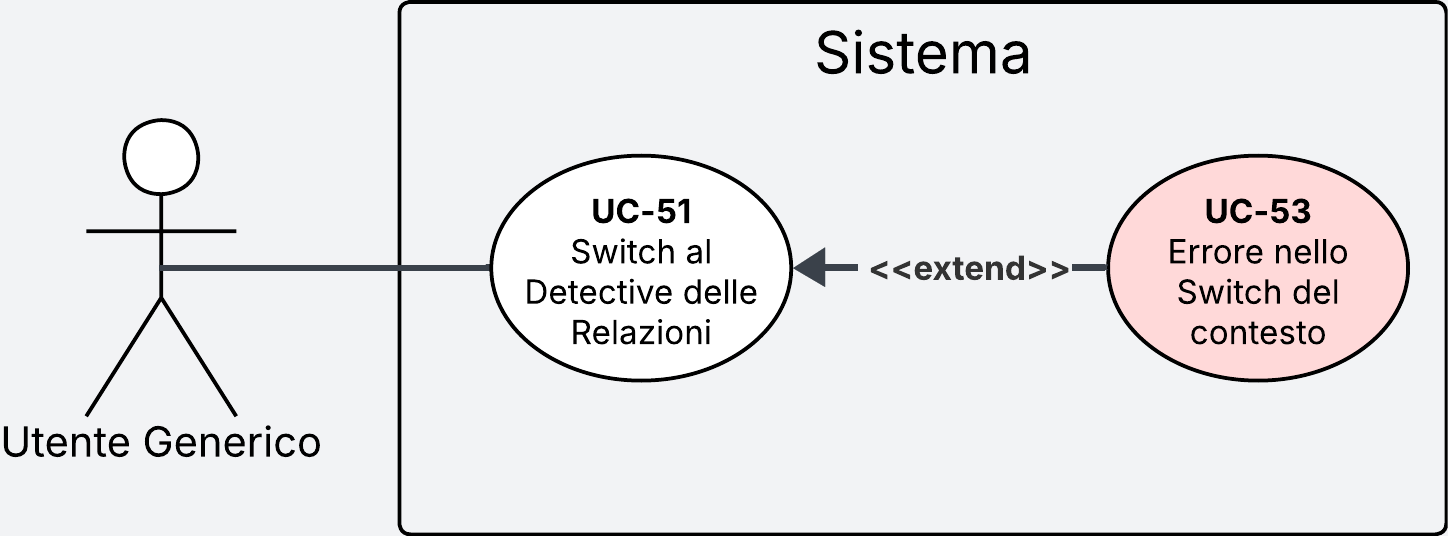
\includegraphics[width=1\textwidth]{use_case/UC-51-detective.png}
    \caption{Diagramma del caso d'uso UC-51}
    \label{fig:UC-51}
\end{figure}
\begin{itemize}
    \item \textbf{Attore principale:} \term{Utente} Autenticato
    \item \textbf{Pre-condizioni:}
    \begin{itemize}
        \item Il sistema è attivo.
        \item Una chat con il chatbot è aperta
        \item Il contesto attualmente impostato è "Specchio Intelligente"
    \end{itemize}	
    \item \textbf{Post-condizioni:}
    \begin{itemize}
        \item Il sistema ha cambiato il contesto fornito al modello da "Specchio Intelligente" a "Detective delle Relazioni"
    \end{itemize}
    \item \textbf{Scenario principale:} 
    \begin{itemize}
        \item L'attore seleziona la voce per il cambio del contesto
        \item Il sistema imposta come attivo il contesto "Detective delle Relazioni"
    \end{itemize}
    \item \textbf{Scenario secondario:} 
    \begin{itemize}
        \item Errore nello switch di contesto \hyperref[sec:UC-53]{UC-53}
    \end{itemize}
    \item \textbf{Estensioni:} 
    \begin{itemize}
        \item \hyperref[sec:UC-53]{UC-53}
    \end{itemize}
    \item \textbf{Trigger:} L'attore vuole cambiare il contesto del chatbot
\end{itemize}

\subsubsection{UC-52 - Switch a "Specchio Intelligente"} \label{sec:UC-52}
\begin{figure}[H]
    \centering
    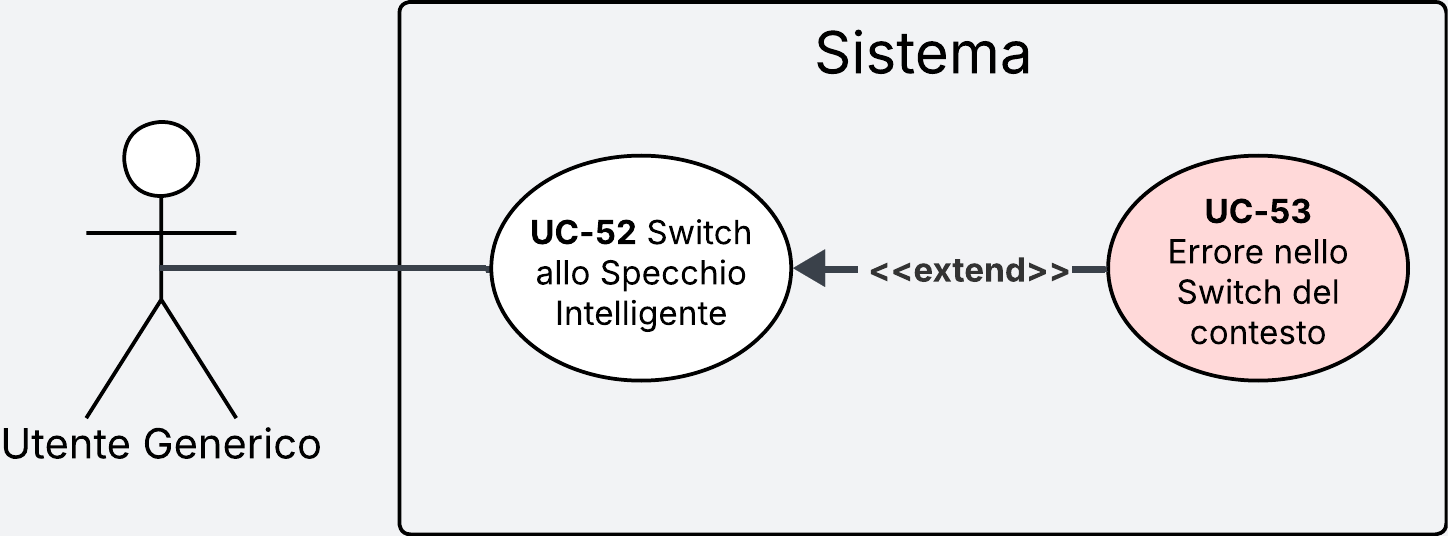
\includegraphics[width=1\textwidth]{use_case/UC-52-detective.png}
    \caption{Diagramma del caso d'uso UC-52}
    \label{fig:UC-52}
\end{figure}
\begin{itemize}
    \item \textbf{Attore principale:} \term{Utente} Autenticato
    \item \textbf{Pre-condizioni:}
    \begin{itemize}
        \item Il sistema è attivo.
        \item Una chat con il chatbot è aperta
        \item Il contesto attualmente impostato è "Detective delle Relazioni"
    \end{itemize}	
    \item \textbf{Post-condizioni:}
    \begin{itemize}
        \item Il sistema ha cambiato il contesto fornito al modello da "Detective delle Relazioni" a "Specchio Intelligente"
    \end{itemize}
    \item \textbf{Scenario principale:} 
    \begin{itemize}
        \item L'attore seleziona la voce per il cambio del contesto
        \item Il sistema imposta come attivo il contesto "Specchio Intelligente"
    \end{itemize}
    \item \textbf{Scenario secondario:} 
    \begin{itemize}
        \item Errore nello switch di contesto \hyperref[sec:UC-53]{UC-53}
    \end{itemize}
    \item \textbf{Estensioni:} 
    \begin{itemize}
        \item \hyperref[sec:UC-53]{UC-53}
    \end{itemize}
    \item \textbf{Trigger:} L'attore vuole cambiare il contesto del chatbot
\end{itemize}

\subsubsection{UC-53 - Errore switch contesto} \label{sec:UC-53}
\begin{itemize}
    \item \textbf{Attore principale:} \term{Utente} Autenticato
    \item \textbf{Pre-condizioni:}
    \begin{itemize}
        \item Il sistema è attivo
        \item L'attore ha richiesto il cambio di contesto
        \item Si \ignoreglossary{verifica} un errore durante l'operazione
    \end{itemize}
    \item \textbf{Post-condizioni:}
    \begin{itemize}
        \item Il sistema notifica l'errore
        \item Il contesto rimane invariato
    \end{itemize}
    \item \textbf{Scenario principale:}
    \begin{itemize}
        \item Il sistema rileva un errore nel cambio del contesto
        \item Il sistema mostra un messaggio di errore
        \item Il sistema mantiene il contesto precedente
        \item Il sistema permette all'attore di ritentare il cambio di contesto
    \end{itemize}
    \item \textbf{Trigger:} L'attore vuole cambiare il contesto del chatbot
\end{itemize}

\subsubsection{UC-54- Creazione nuova chat} \label{subsec:UC-54}
\begin{figure}[H]
    \centering
    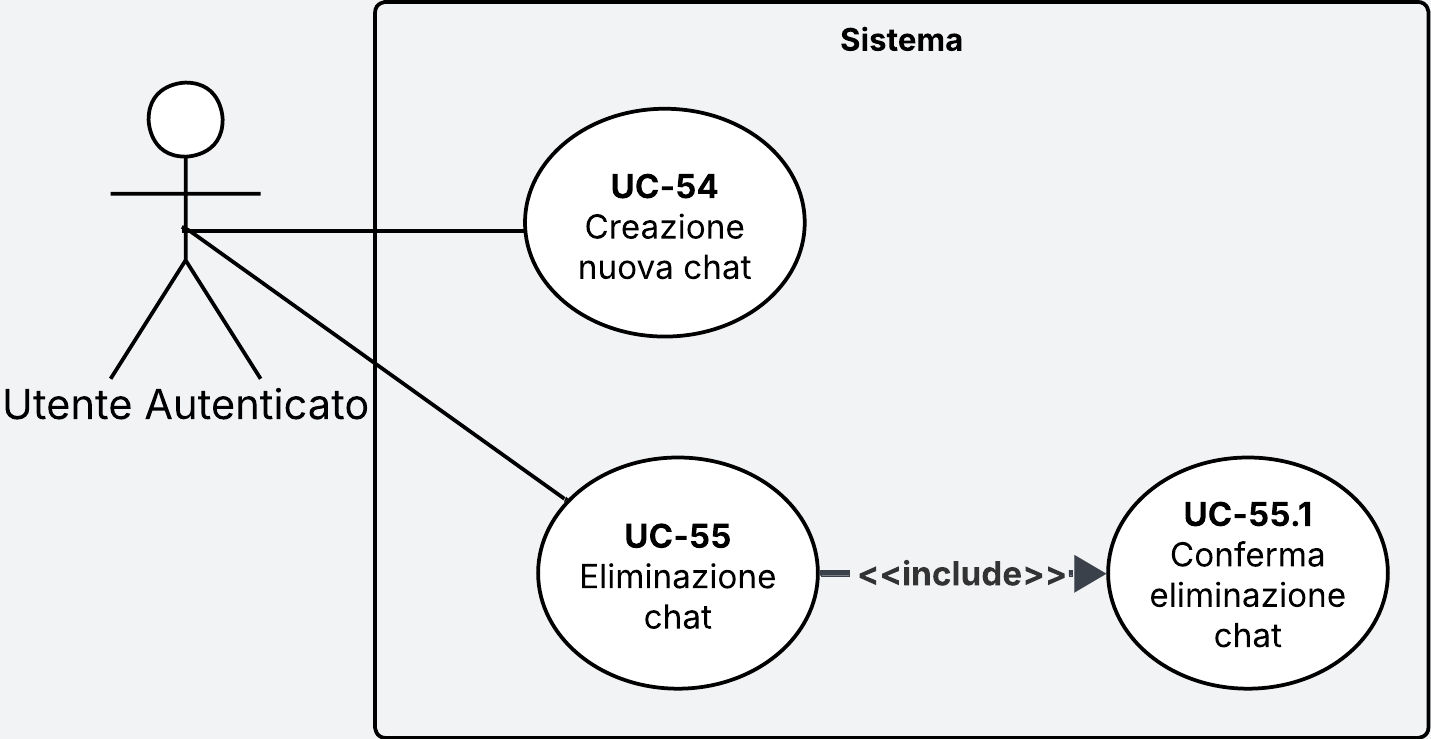
\includegraphics[width=1\textwidth]{use_case/UC-54-55-detective.png}
    \caption{Diagramma dei casi d'uso UC-54 e UC-55}
    \label{fig:UC-54}
\end{figure}
\begin{itemize}
    \item \textbf{Attore principale:} \term{Utente} Autenticato
    \item \textbf{Pre-condizioni:}
    \begin{itemize}
        \item Il sistema è attivo
        \item L'attore si trova nella schermata principale
        \item L'attore ha selezionato la voce per creare una nuova chat
    \end{itemize}
    \item \textbf{Post-condizioni:} 
    \begin{itemize}
        \item Una nuova sessione di chat viene creata
    \end{itemize}
    \item \textbf{Scenario principale:} 
    \begin{itemize}
        \item L'attore seleziona la voce per avviare una nuova conversazione con il chatbot
        \item Il sistema inizializza un nuovo contesto di chat vuoto
        \item Il sistema reindirizza l'attore alla schermata della chat
        \item L'attore visualizza la schermata della chat vuota $\rightarrow$ \hyperref[subsec:UC-56]{UC-56}
    \end{itemize}
    \item \textbf{Inclusioni:} 
    \begin{itemize}
        \item \hyperref[subsec:UC-56]{UC-56}
    \end{itemize}
    \item \textbf{Trigger:} L'attore vuole iniziare una nuova conversazione con il chatbot
\end{itemize}

\subsubsection{UC-55 - Eliminazione chat} \label{subsec:UC-55}
\begin{itemize}
    \item \textbf{Attore principale:} \term{Utente} Autenticato
    \item \textbf{Pre-condizioni:}
    \begin{itemize}
        \item Il sistema è attivo
        \item Esiste almeno una chat nella cronologia
        \item L'attore sta visualizzando la cronologia
    \end{itemize}
    \item \textbf{Post-condizioni:} 
    \begin{itemize}
        \item La chat selezionata e i relativi dati vengono rimossi dal sistema e non sono più visibili
    \end{itemize}
    \item \textbf{Scenario principale:} 
    \begin{itemize}
        \item L'attore seleziona la voce apposita per eliminare una chat dalla cronologia delle chat
        \item L'attore conferma l'intenzione di eliminare la chat $\rightarrow$ \hyperref[subsec:UC-55.1]{UC-55.1}
        \item Il sistema elimina la chat e aggiorna la lista della cronologia
    \end{itemize}
    \item \textbf{Inclusioni:} 
    \begin{itemize}
        \item \hyperref[subsec:UC-55.1]{UC-55.1}
    \end{itemize}
    \item \textbf{Trigger:} L'attore vuole rimuovere una conversazione passata
\end{itemize}

\subsubsection{UC-55.1 - Conferma eliminazione chat} \label{subsec:UC-55.1}
\begin{itemize}
    \item \textbf{Attore principale:} \term{Utente} Autenticato
    \item \textbf{Pre-condizioni:}
    \begin{itemize}
        \item Il sistema è attivo
        \item L'attore ha richiesto l'eliminazione di una chat
    \end{itemize}
    \item \textbf{Post-condizioni:} 
    \begin{itemize}
        \item L'operazione di eliminazione viene confermata al sistema
    \end{itemize}
    \item \textbf{Scenario principale:} 
    \begin{itemize}
        \item Il sistema richiede una conferma esplicita per procedere con l'eliminazione
        \item L'attore conferma l'operazione
    \end{itemize}
    \item \textbf{Trigger:} L'attore vuole confermare l'eliminazione della chat
\end{itemize}

\subsubsection{UC-56 - Visualizzazione contenuto chat} \label{subsec:UC-56}
\begin{tcolorbox}[colback=gray!10,colframe=gray!50,title=Nota]
{\small Il seguente grafico rappresenta il caso d'uso \hyperref[subsec:UC-56]{UC-56} che include diversi casi d'uso quali \hyperref[subsec:UC-56.1]{UC-56.1}, \hyperref[subsec:UC-56.1.1]{UC-56.1.1} e \hyperref[subsec:UC-56.1.2]{UC-56.1.2} la cui descrizione dettagliata è riportata nelle sezioni successive del documento.
Inoltre mostra un caso d'uso d'errore \hyperref[sec:UC-5]{UC-5} la quale descrizione è situata precedentemente nel documento. }
\end{tcolorbox}
\begin{figure}[H]
    \centering
    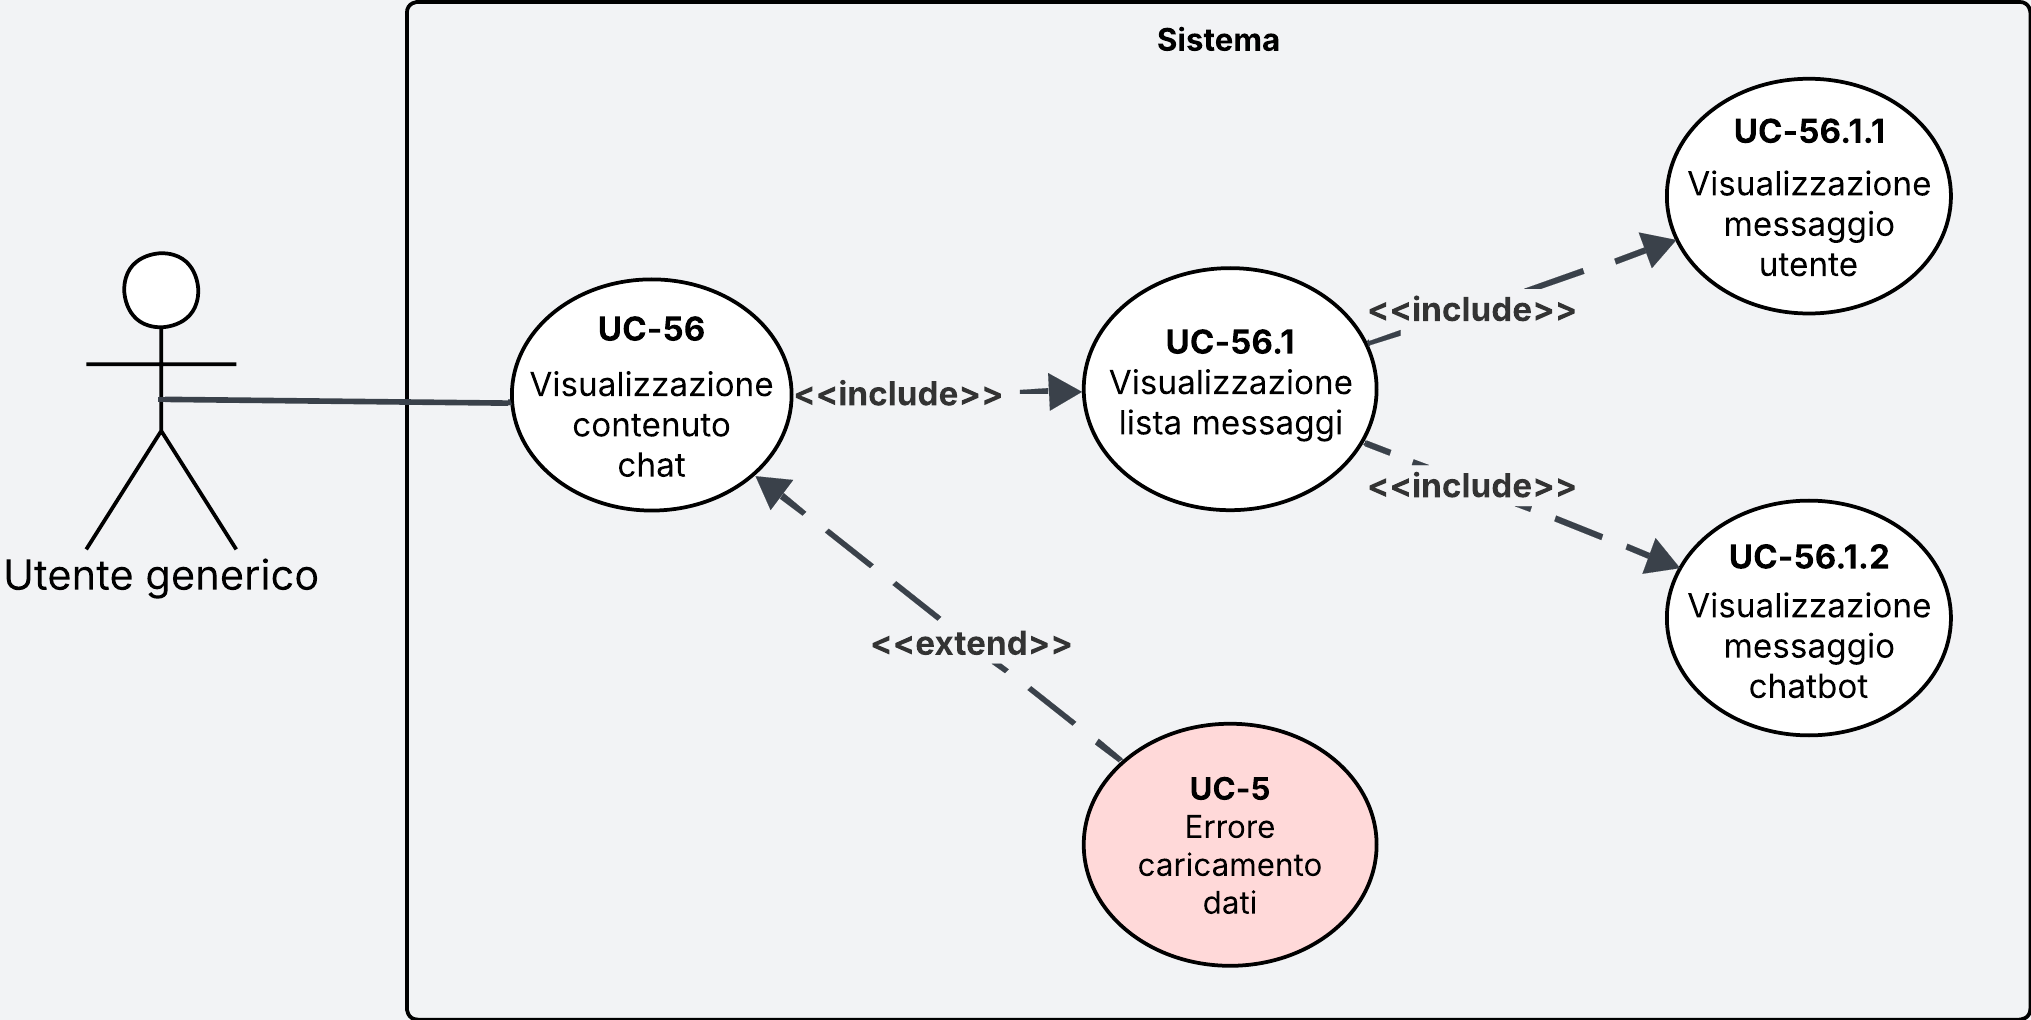
\includegraphics[width=1\textwidth]{use_case/UC-56-detective.png}
    \caption{Diagramma del caso d'uso UC-56}
    \label{fig:UC-56}
\end{figure}
\begin{itemize}
    \item \textbf{Attore principale:} \term{Utente} Autenticato
    \item \textbf{Pre-condizioni:}
    \begin{itemize}
        \item Il sistema è attivo
        \item L'attore ha selezionato una chat (dalla cronologia o una nuova conversazione)
    \end{itemize}
    \item \textbf{Post-condizioni:} 
    \begin{itemize}
        \item L'attore visualizza l'interfaccia della chat con i relativi contenuti
    \end{itemize}
    \item \textbf{Scenario principale:} 
    \begin{itemize}
        \item Il sistema carica il contenuto della chat selezionata
        \item Il sistema visualizza la lista dei messaggi scambiati tra attore e chatbot $\rightarrow$ \hyperref[subsec:UC-56.1]{UC-56.1}
    \end{itemize}
    \item \textbf{Scenario secondario:} 
    \begin{itemize}
        \item Si \ignoreglossary{verifica} un errore nel caricamento del contenuto della chat $\rightarrow$ \hyperref[sec:UC-5]{UC-5}
    \end{itemize}
    \item \textbf{Inclusioni:} 
    \begin{itemize}
        \item \hyperref[subsec:UC-56.1]{UC-56.1}
    \end{itemize}
    \item \textbf{Estensioni:} 
    \begin{itemize}
        \item \hyperref[sec:UC-5]{UC-5}
    \end{itemize}
    \item \textbf{Trigger:} L'attore vuole visualizzare il contenuto di una chat specifica
\end{itemize}

\subsubsection{UC-56.1 - Visualizzazione lista messaggi} \label{subsec:UC-56.1}
\begin{itemize}
    \item \textbf{Attore principale:} \term{Utente} Autenticato
    \item \textbf{Pre-condizioni:} 
    \begin{itemize}
        \item Il sistema è attivo
        \item L'attore sta visualizzando il contenuto della chat
    \end{itemize}
    \item \textbf{Post-condizioni:}
    \begin{itemize}
        \item L'attore visualizza la lista dei messaggi della conversazione avuta con il chatbot
    \end{itemize}
    \item \textbf{Scenario principale:} 
    \begin{itemize}
        \item Il sistema recupera i messaggi dal database
        \item Per ogni messaggio presente, il sistema ne identifica la tipologia (attore o chatbot)
        \item Il sistema visualizza i messaggi dell'attore $\rightarrow$ \hyperref[subsec:UC-56.1.1]{UC-56.1.1}
        \item Il sistema visualizza i messaggi del chatbot $\rightarrow$ \hyperref[subsec:UC-56.1.2]{UC-56.1.2}
        \item L'attore può scorrere tra i messaggi
    \end{itemize}
    \item \textbf{Inclusioni:}
    \begin{itemize}
        \item \hyperref[subsec:UC-56.1.1]{UC-56.1.1}
        \item \hyperref[subsec:UC-56.1.2]{UC-56.1.2}
    \end{itemize}
    \item \textbf{Trigger:} L'attore vuole visualizzare la lista dei messaggi nella chat
\end{itemize}

\subsubsection{UC-56.1.1 - Visualizzazione messaggio \ignoreglossary{Utente}} \label{subsec:UC-56.1.1}
\begin{itemize}
    \item \textbf{Attore principale:} \term{Utente} Autenticato
    \item \textbf{Pre-condizioni:} 
    \begin{itemize}
        \item Il sistema è attivo
        \item Il sistema sta mostrando la lista dei messaggi all'attore
    \end{itemize}
    \item \textbf{Post-condizioni:}
    \begin{itemize}
        \item Il singolo messaggio inviato dall'attore viene mostrato a schermo
    \end{itemize}
    \item \textbf{Scenario principale:} 
    \begin{itemize}
        \item Il sistema mostra il testo del messaggio inviato dall'attore con la formattazione grafica allineata a destra
    \end{itemize}
    \item \textbf{Trigger:} L'attore vuole visualizzare la lista dei messaggi nella chat
\end{itemize}

\subsubsection{UC-56.1.2 - Visualizzazione messaggio chatbot} \label{subsec:UC-56.1.2}
\begin{itemize}
    \item \textbf{Attore principale:} \term{Utente} Autenticato
    \item \textbf{Pre-condizioni:} 
    \begin{itemize}
        \item Il sistema è attivo
        \item Il sistema sta mostrando la lista dei messaggi all'attore
    \end{itemize}
    \item \textbf{Post-condizioni:}
    \begin{itemize}
        \item Il singolo messaggio generato dal chatbot viene mostrato a schermo
    \end{itemize}
    \item \textbf{Scenario principale:} 
    \begin{itemize}
        \item Il sistema mostra il testo del messaggio generato dal chatbot con la formattazione grafica allineata a sinistra
    \end{itemize}
    \item \textbf{Trigger:} L'attore vuole visualizzare la lista dei messaggi nella chat
\end{itemize}

\subsubsection{UC-57 - Visualizzazione cronologia chat} \label{subsec:UC-57}
\begin{figure}[H]
    \centering
    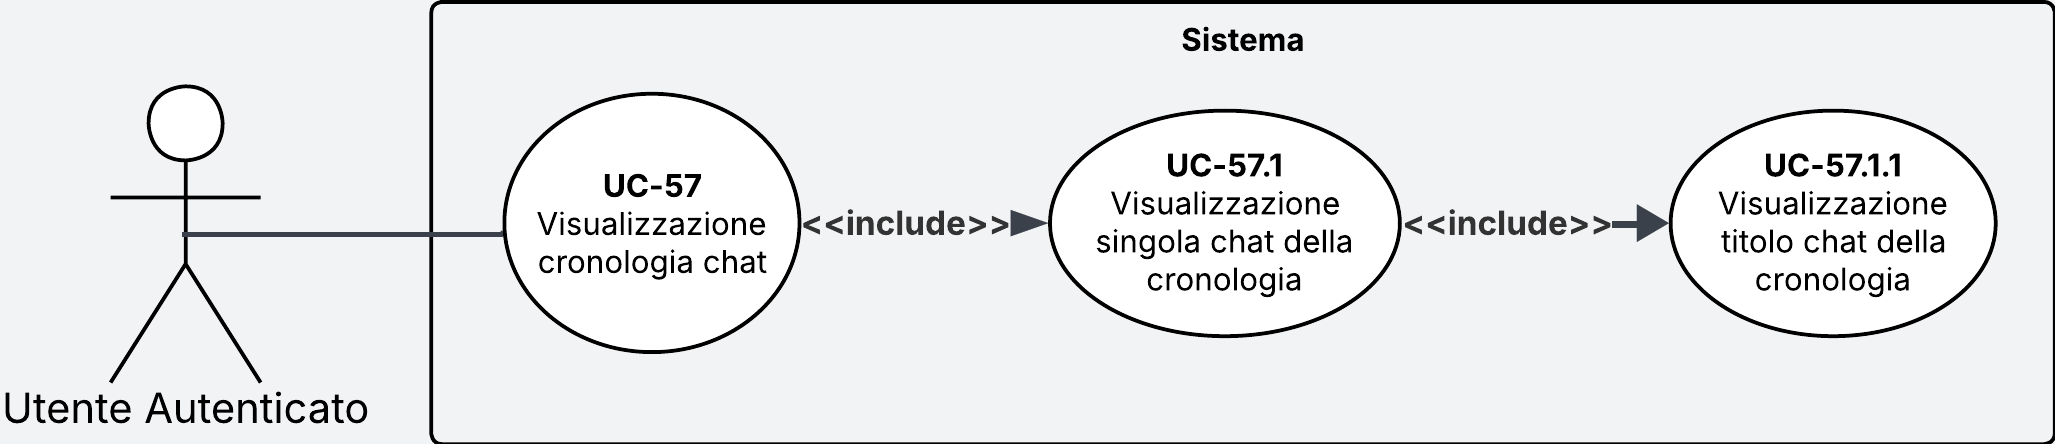
\includegraphics[width=1\textwidth]{use_case/UC-57-detective.png}
    \caption{Diagramma del caso d'uso UC-57}
    \label{fig:UC-57}
\end{figure}
\begin{itemize}
    \item \textbf{Attore principale:} \term{Utente} Autenticato
    \item \textbf{Pre-condizioni:}
    \begin{itemize}
        \item Il sistema è attivo
        \item L'attore ha selezionato la cronologia delle chat
    \end{itemize}
    \item \textbf{Post-condizioni:} 
    \begin{itemize}
        \item Il sistema mostra l'elenco completo delle chat in cronologia
    \end{itemize}
    \item \textbf{Scenario principale:} 
    \begin{itemize}
        \item Il sistema recupera tutte le chat memorizzate
        \item Il sistema visualizza la lista delle chat con un titolo identificativo della chat
        \item L'attore può visualizzare una singola chat dalla lista $\rightarrow$ \hyperref[subsec:UC-57.1]{UC-57.1}
    \end{itemize}
    \item \textbf{Inclusioni:}
    \begin{itemize}
        \item \hyperref[subsec:UC-57.1]{UC-57.1}
    \end{itemize}
    \item \textbf{Trigger:} L'attore vuole visualizzare la cronologia delle chat
\end{itemize}

\subsubsection{UC-57.1 - Visualizzazione singola chat della cronologia} \label{subsec:UC-57.1}
\begin{itemize}
    \item \textbf{Attore principale:} \term{Utente} Autenticato
    \item \textbf{Pre-condizioni:}
    \begin{itemize}
        \item Il sistema è attivo
        \item La cronologia delle chat è visibile
    \end{itemize}
    \item \textbf{Post-condizioni:} 
    \begin{itemize}
        \item L'attore ha visualizzato una singola chat
    \end{itemize}
    \item \textbf{Scenario principale:} 
    \begin{itemize}
        \item Il sistema recupera le informazioni della chat da visualizzare
        \item Il sistema mostra il titolo della chat nella lista $\rightarrow$ \hyperref[subsec:UC-57.1.1]{UC-57.1.1}
    \end{itemize}
    \item \textbf{Inclusioni:}
    \begin{itemize}
        \item \hyperref[subsec:UC-57.1.1]{UC-57.1.1}
    \end{itemize}
    \item \textbf{Trigger:} L'attore vuole visualizzare una singola chat dalla cronologia

\end{itemize}

\subsubsection{UC-57.1.1 - Visualizzazione titolo chat della cronologia} \label{subsec:UC-57.1.1}
\begin{itemize}
    \item \textbf{Attore principale:} \term{Utente} Autenticato
    \item \textbf{Pre-condizioni:}
    \begin{itemize}
        \item Il sistema è attivo
        \item L'attore ha selezionato la cronologia delle chat
        \item La cronologia delle chat è visibile
        \item Le chat sono caricate
    \end{itemize}
    \item \textbf{Post-condizioni:} 
    \begin{itemize}
        \item L'attore ha visualizzato il titolo di una chat
    \end{itemize}
    \item \textbf{Scenario principale:} 
    \begin{itemize}
        \item Il sistema mostra il titolo della chat nella lista
    \end{itemize}
    \item \textbf{Trigger:} L'attore vuole visualizzare il titolo di una chat dalla cronologia
\end{itemize}

% ========================== UC-G: Guide ==============================

\subsubsection{UC-58 - Visualizzazione lista community} \label{sec:UC-58}
\begin{figure}[H]
    \centering
    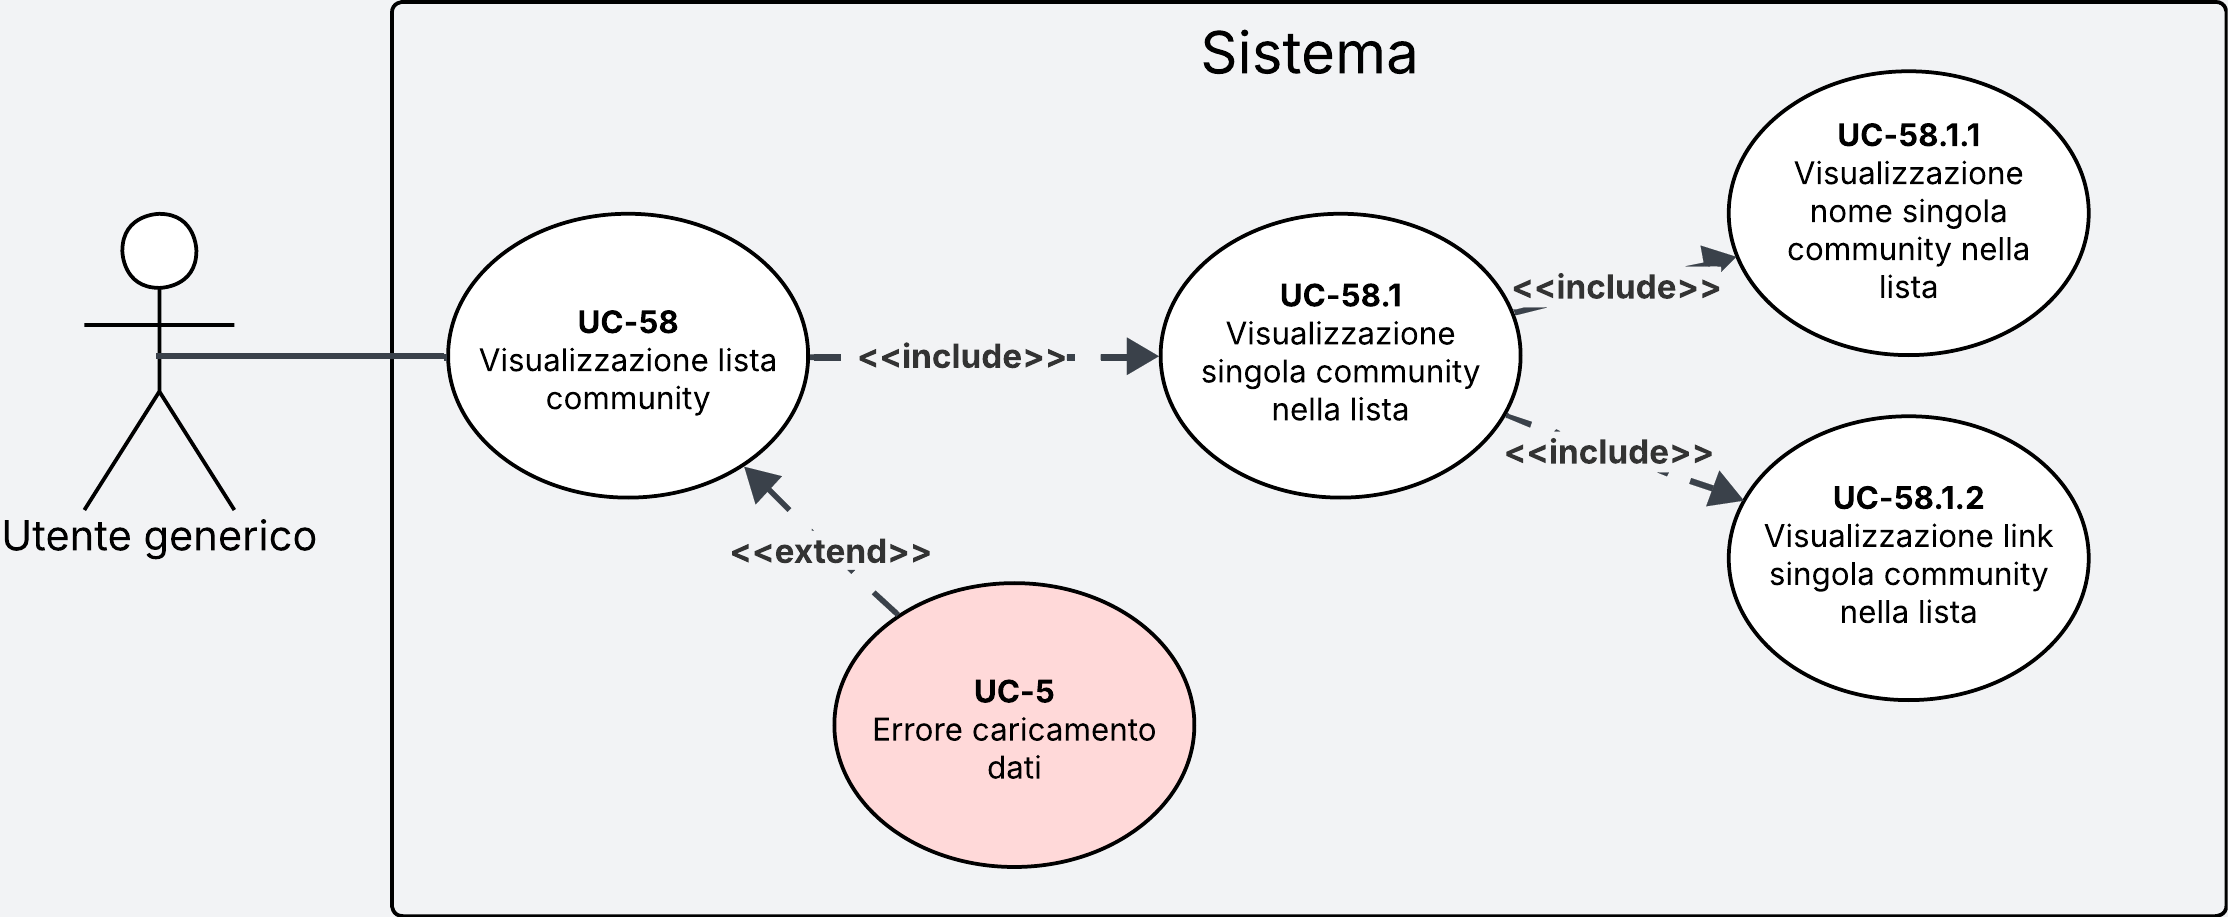
\includegraphics[width=1\textwidth]{use_case/UC-58-coraggio.png}
    \caption{Diagramma del caso d'uso UC-58}
    \label{fig:UC-58}
\end{figure}
\begin{itemize}
    \item \textbf{Attore principale:} \term{Utente} Generico
    \item \textbf{Pre-condizioni:}
    \begin{itemize}
        \item Il sistema è attivo
        \item L'attore ha selezionato la sezione dedicata alle community
    \end{itemize}
    \item \textbf{Post-condizioni:}
    \begin{itemize}
        \item L'attore visualizza l'elenco delle community disponibili
    \end{itemize}
    \item \textbf{Scenario principale:} 
    \begin{itemize}
        \item Il sistema recupera l'elenco delle community da visualizzare 
        \item Il sistema visualizza a schermo la lista delle community $\rightarrow$ \hyperref[subsec:UC-58.1]{UC-58.1}
    \end{itemize}
    \item \textbf{Scenario secondario:} 
    \begin{itemize}
        \item Il sistema rileva un errore nel caricamento dei dati $\rightarrow$ \hyperref[sec:UC-5]{UC-5}
    \end{itemize}
    \item \textbf{Inclusioni:} 
    \begin{itemize}
        \item \hyperref[subsec:UC-58.1]{UC-58.1}
    \end{itemize}
    \item \textbf{Estensioni:} 
    \begin{itemize}
        \item \hyperref[sec:UC-5]{UC-5}
    \end{itemize}
    \item \textbf{Trigger:} L'attore vuole vedere la lista delle community esistenti
\end{itemize}

\subsubsection{UC-58.1 - Visualizzazione singola community nella lista} \label{subsec:UC-58.1}
\begin{itemize}
    \item \textbf{Attore principale:} \term{Utente} Generico
    \item \textbf{Pre-condizioni:} 
    \begin{itemize}
        \item Il sistema è attivo
        \item L'attore si trova all'interno della sezione dedicata alle community
        \item Il sistema ha recuperato le informazioni relative alle community da visualizzare
    \end{itemize}
    \item \textbf{Post-condizioni:}
    \begin{itemize}
        \item L'attore visualizza una singola community all'interno della lista
    \end{itemize}
    \item \textbf{Scenario principale:} 
    \begin{itemize}
        \item L'attore visualizza una singola community all'interno della lista
        \item L'attore visualizza il nome della community  $\rightarrow$ \hyperref[subsec:UC-58.1.1]{UC-58.1.1}
        \item L'attore visualizza il link della community  $\rightarrow$ \hyperref[subsec:UC-58.1.2]{UC-58.1.2}
    \end{itemize}
    \item \textbf{Inclusioni:} 
    \begin{itemize}
        \item \hyperref[subsec:UC-58.1.1]{UC-58.1.1}
        \item \hyperref[subsec:UC-58.1.2]{UC-58.1.2}
    \end{itemize}
    \item \textbf{Trigger:} L'attore vuole vedere la lista delle community esistenti
\end{itemize}

\subsubsection{UC-58.1.1 - Visualizzazione nome singola community nella lista} \label{subsec:UC-58.1.1}
\begin{itemize}
    \item \textbf{Attore principale:} \term{Utente} Generico
    \item \textbf{Pre-condizioni:} 
    \begin{itemize}
        \item Il sistema è attivo
        \item L'attore si trova all'interno della sezione dedicata alle community
        \item Il sistema ha recuperato le informazioni relative alle community da visualizzare
        \item L'attore visualizza una singola community all'interno della lista
    \end{itemize}
    \item \textbf{Post-condizioni:}
    \begin{itemize}
        \item L'attore visualizza il nome della singola community dalla lista
    \end{itemize}
    \item \textbf{Scenario principale:} 
    \begin{itemize}
        \item L'attore visualizza dalla lista delle community, il nome di una singola community
    \end{itemize}
\end{itemize}

\subsubsection{UC-58.1.2 - Visualizzazione link singola community nella lista} \label{subsec:UC-58.1.2}
\begin{itemize}
    \item \textbf{Attore principale:} \term{Utente} Generico
    \item \textbf{Pre-condizioni:} 
    \begin{itemize}
        \item Il sistema è attivo
        \item L'attore ha selezionato la sezione dedicata alle community
        \item L'attore visualizza l'elenco delle community online esterne
        \item L'attore visualizza una singola community all'interno della lista
    \end{itemize}
    \item \textbf{Post-condizioni:}
    \begin{itemize}
        \item L'attore visualizza il link della singola community all'interno della lista
    \end{itemize}
    \item \textbf{Scenario principale:} 
    \begin{itemize}
        \item L'attore visualizza all'interno della lista delle community, il link di una singola community
    \end{itemize}
\end{itemize}

\subsubsection{UC-59 - Apertura link della community} \label{sec:UC-59}
\begin{figure}[H]
    \centering
    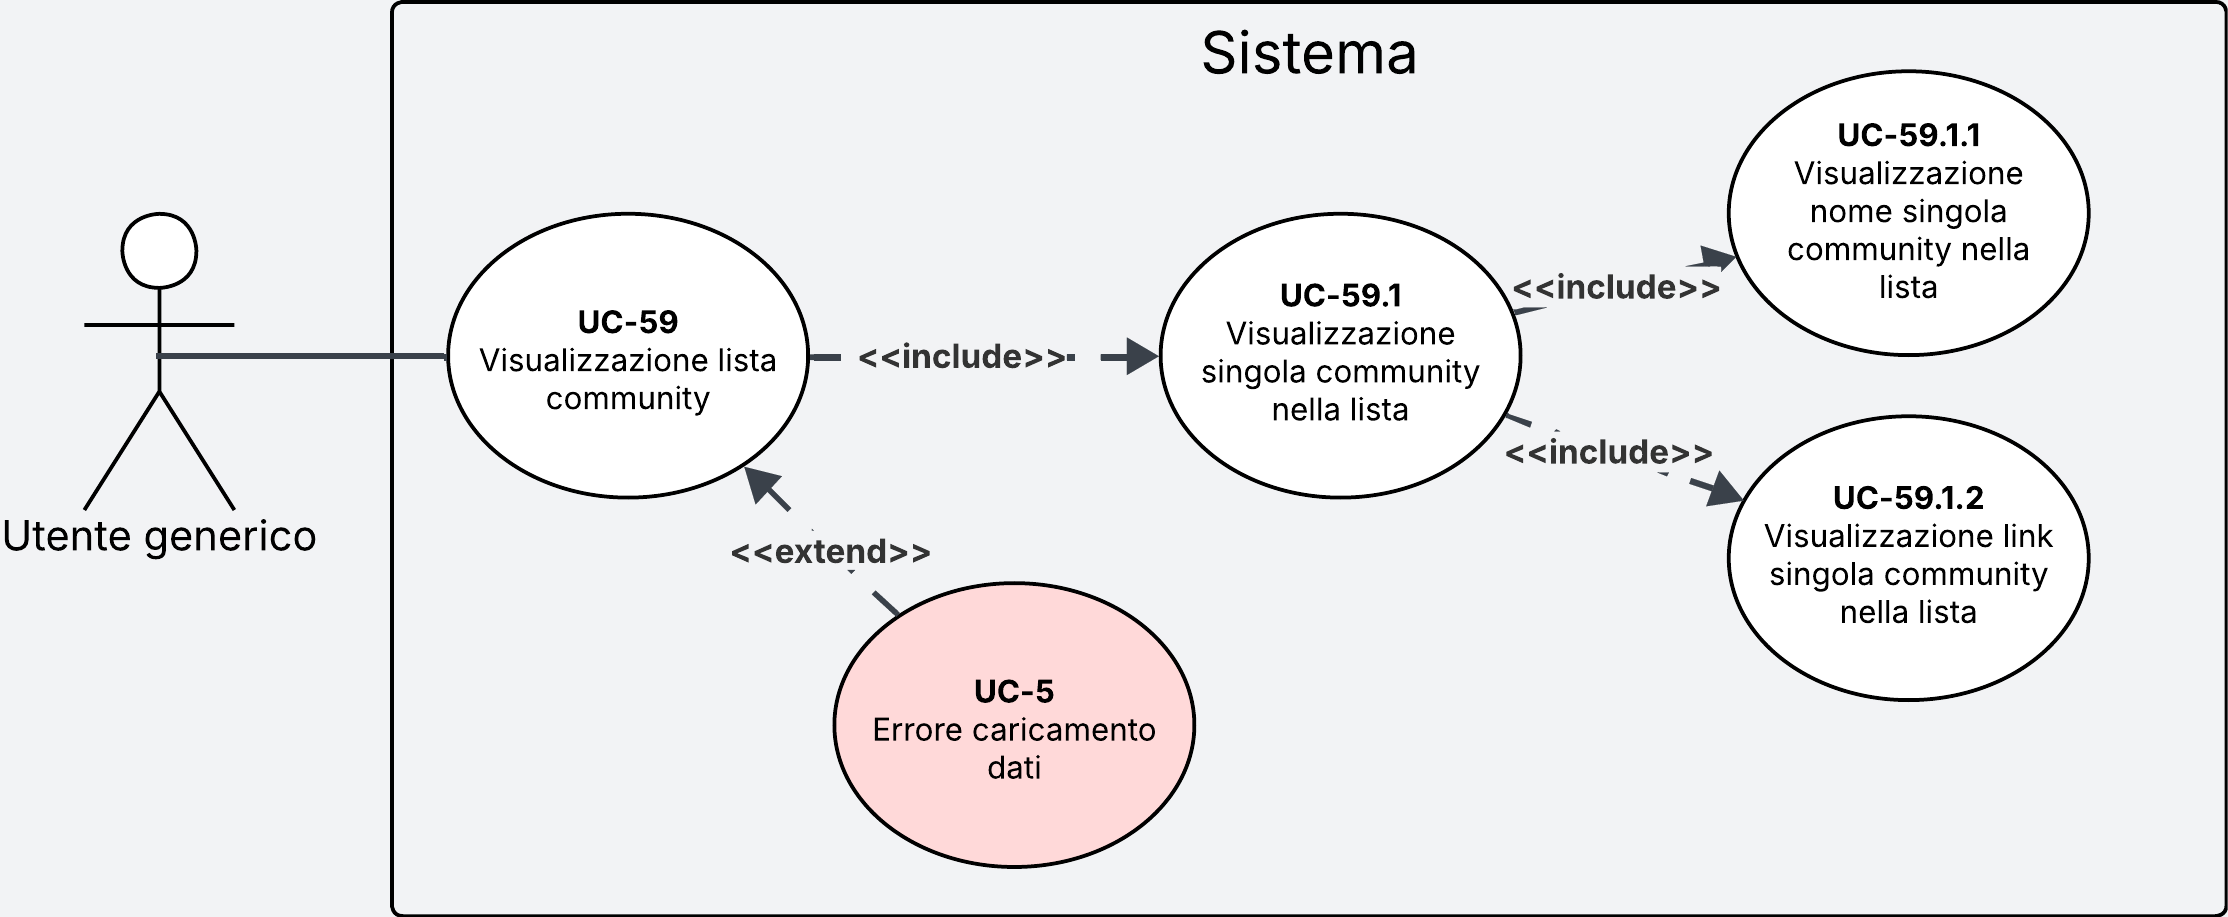
\includegraphics[width=1\textwidth]{use_case/UC-59-coraggio.png}
    \caption{Diagramma del caso d'uso UC-59}
    \label{fig:UC-59}
\end{figure}
\begin{itemize}
    \item \textbf{Attore principale:} \term{Utente} Generico
    \item \textbf{Pre-condizioni:}
    \begin{itemize}
        \item Il sistema è attivo
        \item L'attore visualizza la lista delle community
        \item L'attore visualizza una singola community all'interno della lista
        \item L'attore visualizza il link della singola community all'interno della lista
    \end{itemize}
    \item \textbf{Post-condizioni:}
    \begin{itemize}
        \item L'attore visualizza il sito web relativo al link della community selezionata
    \end{itemize}
    \item \textbf{Scenario principale:} 
    \begin{itemize}
        \item L'attore seleziona il link di una community specifica dalla lista
        \item L'attore visita il link relativo alla community che è stata selezionata
    \end{itemize}
    \item \textbf{Trigger:} L'attore vuole visitare il link di una community
\end{itemize}

\subsubsection{UC-60 - Visualizzazione lista leggi} \label{sec:UC-60}
\begin{figure}[H]
    \centering
    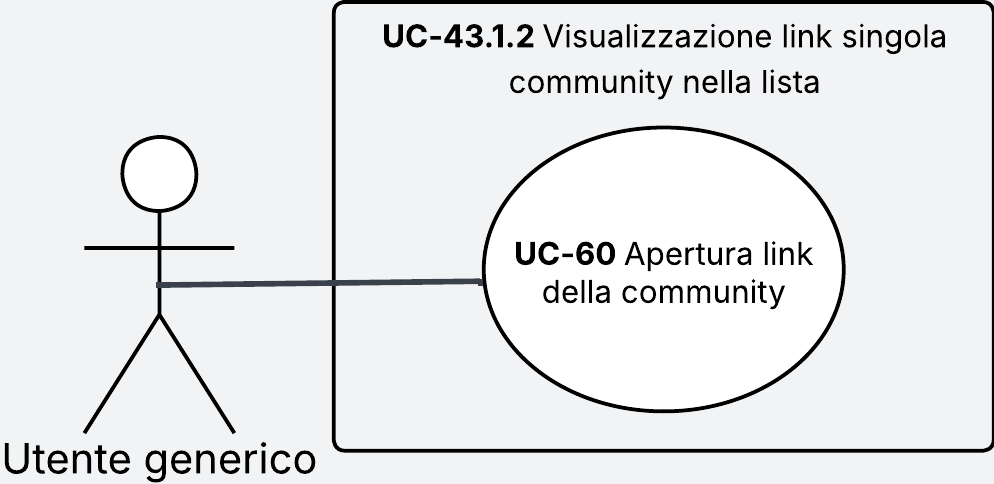
\includegraphics[width=1\textwidth]{use_case/UC-60-coraggio.png}
    \caption{Diagramma del caso d'uso UC-60}
    \label{fig:UC-60}
\end{figure}
\begin{itemize}
    \item \textbf{Attore principale:} \term{Utente} Generico
    \item \textbf{Pre-condizioni:}
    \begin{itemize}
        \item Il sistema è attivo
        \item L'attore ha selezionato la sezione informativa sulle normative vigenti
    \end{itemize}
    \item \textbf{Post-condizioni:}
    \begin{itemize}
        \item L'attore visualizza l'elenco delle leggi e dei diritti pertinenti
    \end{itemize}
    \item \textbf{Scenario principale:} 
    \begin{itemize}
        \item Il sistema recupera l'elenco delle normative dal database
        \item Il sistema visualizza le voci della lista delle leggi $\rightarrow$ \hyperref[subsec:UC-60.1]{UC-60.1}
        \item L'attore può scorrere la lista per cercare l'argomento di interesse
    \end{itemize}
    \item \textbf{Inclusioni:} 
    \begin{itemize}
        \item \hyperref[subsec:UC-60.1]{UC-60.1}
    \end{itemize}
    \item \textbf{Trigger:} L'attore vuole visualizzare la lista delle leggi
\end{itemize}

\subsubsection{UC-60.1 - Visualizzazione singola legge nella lista} \label{subsec:UC-60.1}
\begin{itemize}
    \item \textbf{Attore principale:} \term{Utente} Generico
    \item \textbf{Pre-condizioni:} 
    \begin{itemize}
        \item Il sistema è attivo
        \item Il sistema sta mostrando la lista delle leggi
    \end{itemize}
    \item \textbf{Post-condizioni:}
    \begin{itemize}
        \item L'attore visualizza il titolo
    \end{itemize}
    \item \textbf{Scenario principale:} 
    \begin{itemize}
        \item Il sistema mostra il titolo della legge
        \item L'attore può selezionare una legge per aprirne i dettagli
    \end{itemize}
    \item \textbf{Trigger:} L'attore visualizza la lista delle leggi
\end{itemize}

\subsubsection{UC-61 - Visualizzazione dettagli legge} \label{sec:UC-61}
\begin{figure}[H]
    \centering
    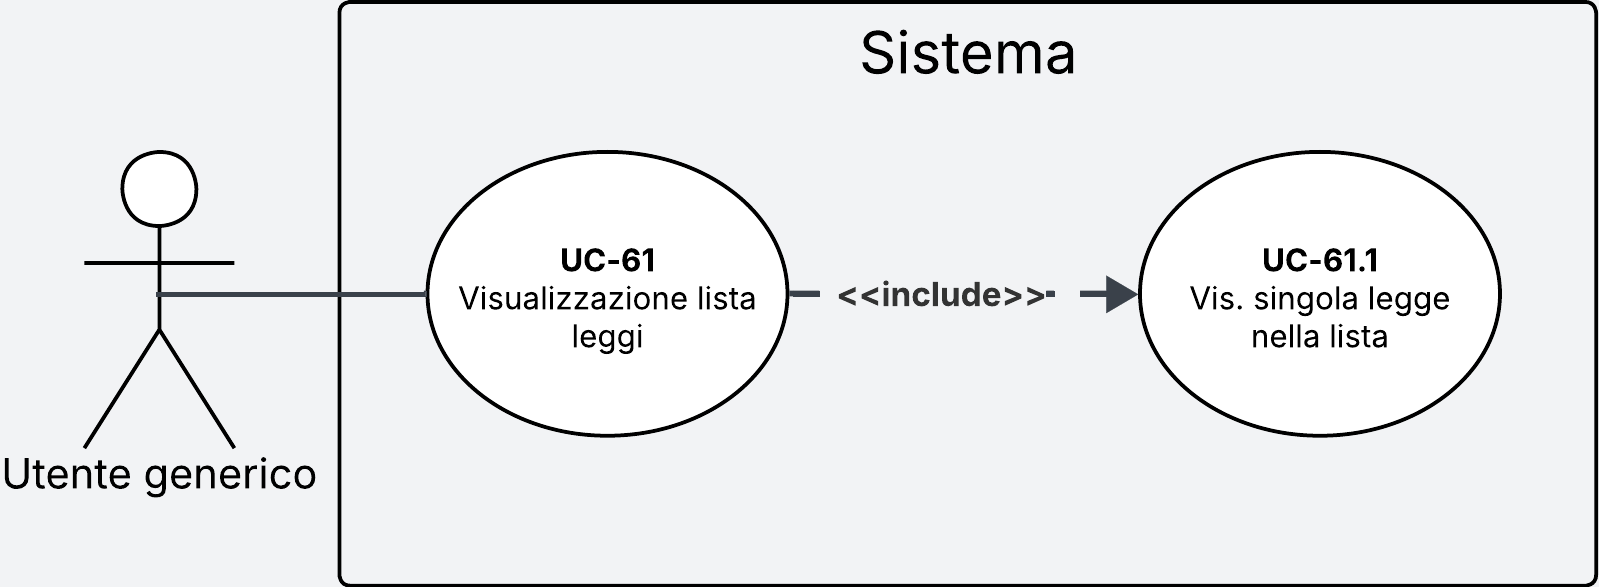
\includegraphics[width=1\textwidth]{use_case/UC-61-coraggio.png}
    \caption{Diagramma del caso d'uso UC-61}
    \label{fig:UC-61}
\end{figure}
\begin{itemize}
    \item \textbf{Attore principale:} \term{Utente} Generico
    \item \textbf{Pre-condizioni:}
    \begin{itemize}
        \item Il sistema è attivo
        \item L'attore visualizza la lista delle leggi
        \item L'attore seleziona una legge dalla lista
    \end{itemize}
    \item \textbf{Post-condizioni:}
    \begin{itemize}
        \item L'attore visualizza interamente i dettagli della legge
    \end{itemize}
    \item \textbf{Scenario principale:} 
    \begin{itemize}
        \item L'attore seleziona una normativa specifica dalla lista
        \item Il sistema recupera il contenuto dettagliato della legge
        \item Il sistema presenta la schermata di dettaglio con il testo esplicativo completo
    \end{itemize}
    \item \textbf{Scenario secondario:} 
    \begin{itemize}
         \item Si \ignoreglossary{verifica} un errore nel caricamento dei dati dal database $\rightarrow$ \hyperref[sec:UC-5]{UC-5}
    \end{itemize}
    \item \textbf{Estensioni:}
    \begin{itemize}
     \item \hyperref[sec:UC-5]{UC-5}
    \end{itemize}
    \item \textbf{Trigger:} L'attore vuole approfondire il contenuto di una legge
\end{itemize}

\subsubsection{UC-62 - Visualizzazione lista contatti d'emergenza} \label{sec:UC-62}
\begin{tcolorbox}[colback=gray!10,colframe=gray!50,title=Nota]
{\small Il caso d'uso \hyperref[sec:UC-62]{UC-62} include il caso d'uso \hyperref[subsec:UC-62.1]{UC-62.1}, si mostrano anche ulteriori casi d'uso correlati (\hyperref[subsec:UC-62.1.1]{UC-62.1.1} e \hyperref[subsec:UC-62.1.2]{UC-62.1.2}), la cui descrizione dettagliata è riportata nelle sezioni successive del documento.}
\end{tcolorbox}
\begin{figure}[H]
    \centering
    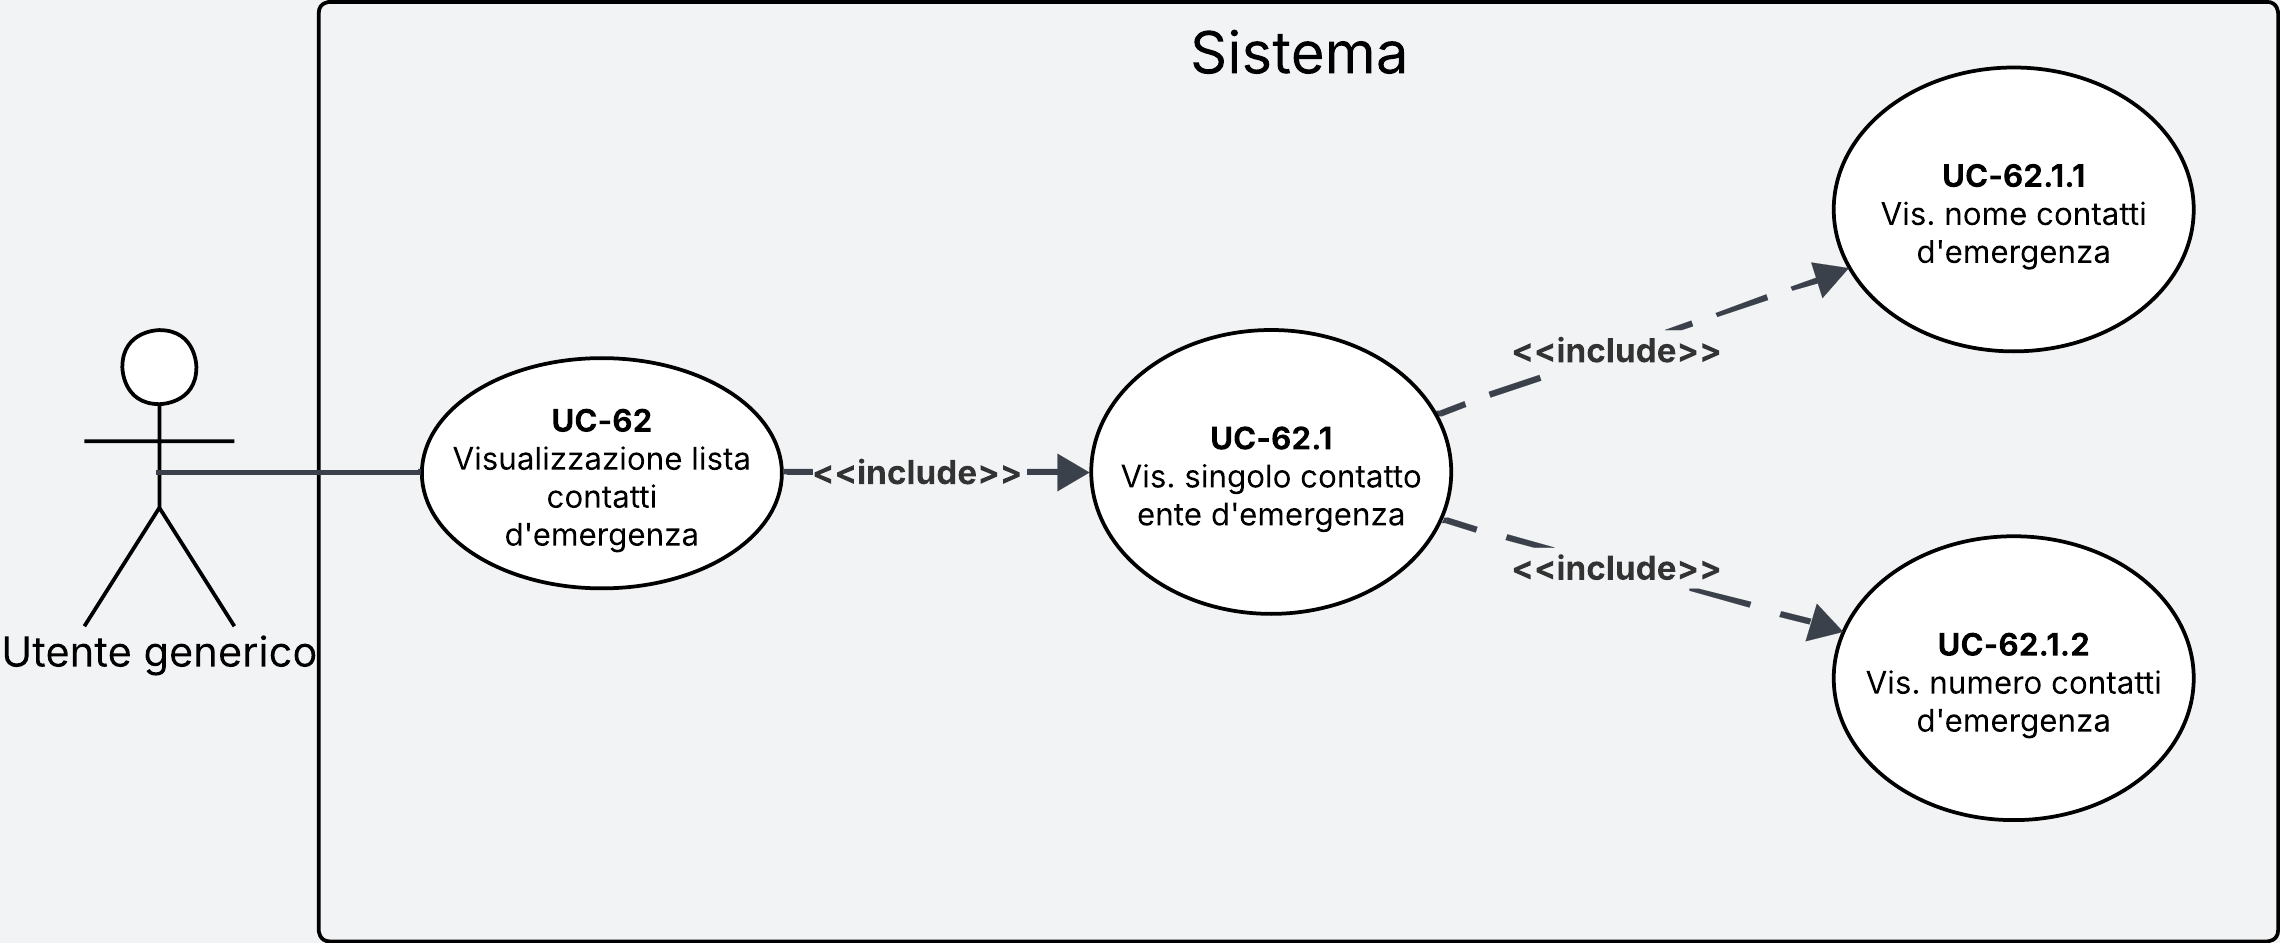
\includegraphics[width=1\textwidth]{use_case/UC-62-coraggio.png}
    \caption{Diagramma del caso d'uso UC-62}
    \label{fig:UC-62}
\end{figure}
\begin{itemize}
    \item \textbf{Attore principale:} \term{Utente} Generico
    \item \textbf{Pre-condizioni:}
    \begin{itemize}
        \item Il sistema è attivo
        \item L'attore ha selezionato la sezione dei numeri utili/emergenza
    \end{itemize}
    \item \textbf{Post-condizioni:}
    \begin{itemize}
        \item L'attore visualizza l'elenco dei numeri di emergenza
    \end{itemize}
    \item \textbf{Scenario principale:} 
    \begin{itemize}
        \item Il sistema recupera la lista dei contatti di emergenza nazionali
        \item Il sistema recupera la lista dei numeri dei contatti fidati personali 
        \item Il sistema visualizza le voci della lista $\rightarrow$ \hyperref[subsec:UC-62.1]{UC-62.1}
    \end{itemize}
    \item \textbf{Inclusioni:} 
    \begin{itemize}
        \item \hyperref[subsec:UC-62.1]{UC-62.1}
    \end{itemize}
    \item \textbf{Trigger:} L'attore vuole consultare i contatti di emergenza
\end{itemize}

\subsubsection{UC-62.1 - Visualizzazione singolo contatto ente d'emergenza} \label{subsec:UC-62.1}
\begin{itemize}
    \item \textbf{Descrizione:} Questo caso d'uso generalizza la visualizzazione di un contatto, definendo la struttura comune (nome e numero) per qualsiasi tipo di contatto d'emergenza.
    \item \textbf{Attore principale:} \term{Utente} Generico
    \item \textbf{Pre-condizioni:} 
    \begin{itemize}
        \item Il sistema è attivo
        \item Il sistema sta renderizzando la lista dei contatti degli enti d'emergenza
    \end{itemize}
    \item \textbf{Post-condizioni:}
    \begin{itemize}
        \item I dettagli essenziali dell'ente sono visibili a schermo
    \end{itemize}
    \item \textbf{Scenario principale:} 
    \begin{itemize}
        \item Il sistema visualizza il nome identificativo del contatto $\rightarrow$ \hyperref[subsec:UC-62.1.1]{UC-62.1.1}
        \item Il sistema visualizza il numero telefonico associato al contatto $\rightarrow$ \hyperref[subsec:UC-62.1.2]{UC-62.1.2}
    \end{itemize}
    \item \textbf{Inclusioni:}
    \begin{itemize}
        \item \hyperref[subsec:UC-62.1.1]{UC-62.1.1}
        \item \hyperref[subsec:UC-62.1.2]{UC-62.1.2}
    \end{itemize}
\end{itemize}

\subsubsection{UC-62.1.1 - Visualizzazione nome contatti d'emergenza} \label{subsec:UC-62.1.1}
\begin{itemize}
    \item \textbf{Attore principale:} \term{Utente} Generico
    \item \textbf{Pre-condizioni:} 
    \begin{itemize}
        \item Il sistema è attivo
        \item Il sistema sta visualizzando un contatto d'emergenza
    \end{itemize}
    \item \textbf{Post-condizioni:}
    \begin{itemize}
        \item Il nome del contatto è visibile
    \end{itemize}
    \item \textbf{Scenario principale:} 
    \begin{itemize}
        \item Il sistema mostra la stringa di testo corrispondente al nome dell'ente o della persona
    \end{itemize}
    \item \textbf{Trigger:} L'attore vuole visualizzare un contatto d'emergenza
\end{itemize}

\subsubsection{UC-62.1.2 - Visualizzazione numero contatti d'emergenza} \label{subsec:UC-62.1.2}
\begin{itemize}
    \item \textbf{Attore principale:} \term{Utente} Generico
    \item \textbf{Pre-condizioni:} 
    \begin{itemize}
        \item Il sistema è attivo
        \item Il sistema sta visualizzando un contatto d'emergenza
    \end{itemize}
    \item \textbf{Post-condizioni:}
    \begin{itemize}
        \item Il numero di telefono è visibile
    \end{itemize}
    \item \textbf{Scenario principale:} 
    \begin{itemize}
        \item Il sistema mostra le cifre del numero telefonico associato al contatto
    \end{itemize}
    \item \textbf{Trigger:} L'attore vuole visualizzare un contatto d'emergenza
\end{itemize}

\subsubsection{UC-63 - Composizione automatica numero contatto} \label{sec:UC-63}
\begin{figure}[H]
    \centering
    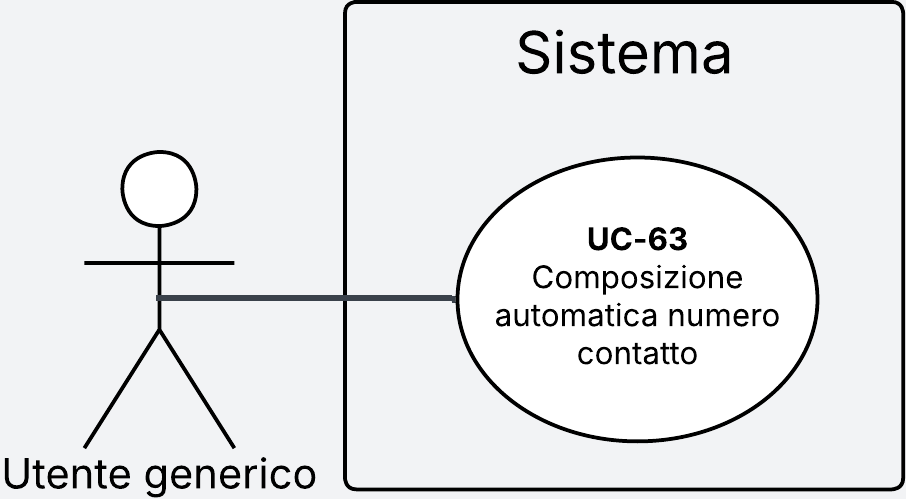
\includegraphics[width=1\textwidth]{use_case/UC-63-coraggio.png}
    \caption{Diagramma del caso d'uso UC-63}
    \label{fig:UC-63}
\end{figure}
\begin{itemize}
    \item \textbf{Attore principale:} \term{Utente} Generico
    \item \textbf{Pre-condizioni:}
    \begin{itemize}
        \item Il sistema è attivo
        \item L'attore visualizza la lista dei contatti d'emergenza
    \end{itemize}
    \item \textbf{Post-condizioni:}
    \begin{itemize}
        \item Il sistema compila il numero sul dispositivo
    \end{itemize}
    \item \textbf{Scenario principale:} 
    \begin{itemize}
        \item L'attore interagisce con un contatto
        \item Il sistema rileva il numero associato
        \item Il sistema compila il numero sul dispositivo dell'attore
    \end{itemize}
    \item \textbf{Trigger:} L'attore vuole chiamare un contatto d'emergenza
\end{itemize}

\subsubsection{UC-64 - Visualizzazione lista materiale informativo} \label{sec:UC-64}
\begin{figure}[H]
    \centering
    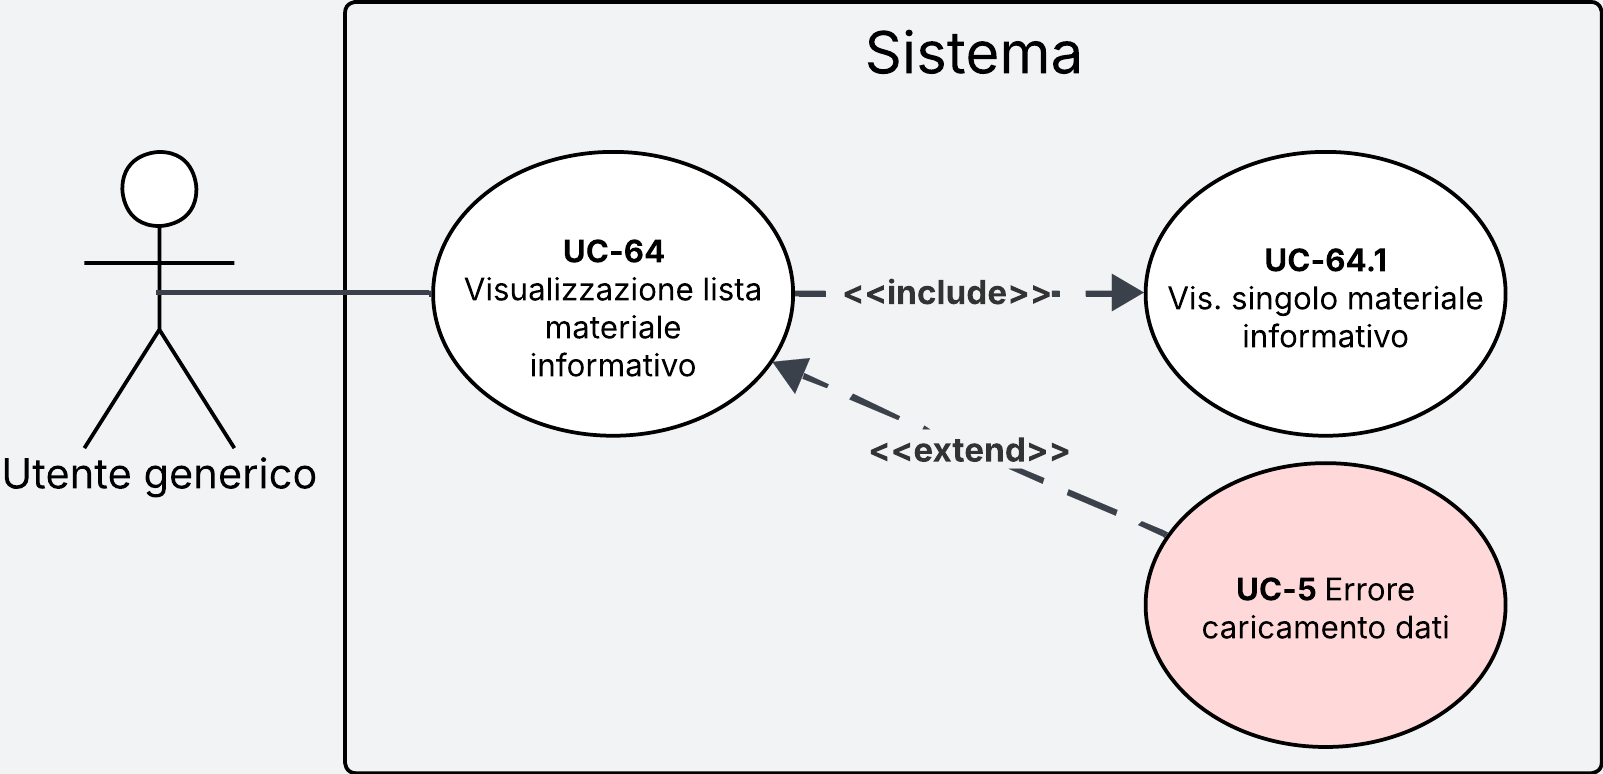
\includegraphics[width=1\textwidth]{use_case/UC-64-coraggio.png}
    \caption{Diagramma del caso d'uso UC-64}
    \label{fig:UC-64}
\end{figure}
\begin{itemize}
    \item \textbf{Attore principale:} \term{Utente} Generico
    \item \textbf{Pre-condizioni:}
    \begin{itemize}
        \item Il sistema è attivo
        \item L'attore ha selezionato la sezione del materiale informativo
    \end{itemize}
    \item \textbf{Post-condizioni:}
    \begin{itemize}
        \item L'attore visualizza l'elenco dei materiali multimediali o testuali disponibili
    \end{itemize}
    \item \textbf{Scenario principale:} 
    \begin{itemize}
        \item Il sistema recupera l'elenco delle risorse disponibili dal server
        \item Il sistema visualizza la lista dei materiali disponibili 
        \item L'attore può visualizzare singolarmente ogni materiale nella lista $\rightarrow$ \hyperref[subsec:UC-64.1]{UC-64.1}
        \item L'attore può scorrere la lista per trovare il contenuto di interesse
    \end{itemize}
    \item \textbf{Scenario secondario:} 
    \begin{itemize}
        \item Si \ignoreglossary{verifica} un errore nel caricamento dei dati dal database $\rightarrow$ \hyperref[sec:UC-5]{UC-5}
    \end{itemize}
    \item \textbf{Inclusioni:}
     \begin{itemize}
         \item \hyperref[subsec:UC-64.1]{UC-64.1}
     \end{itemize}
     \item \textbf{Estensioni:}
     \begin{itemize}
         \item \hyperref[sec:UC-5]{UC-5}
     \end{itemize}
    \item \textbf{Trigger:} L'attore vuole consultare risorse educative o di supporto
\end{itemize}

\subsubsection{UC-64.1 - Visualizzazione singolo materiale informativo} \label{subsec:UC-64.1}
\begin{itemize}
    \item \textbf{Attore principale:} \term{Utente} Generico
    \item \textbf{Pre-condizioni:} 
    \begin{itemize}
        \item Il sistema è attivo
        \item Il sistema sta renderizzando la lista dei materiali
    \end{itemize}
    \item \textbf{Post-condizioni:}
    \begin{itemize}
        \item L'attore visualizza il titolo e il formato del materiale
    \end{itemize}
    \item \textbf{Scenario principale:} 
    \begin{itemize}
        \item Il sistema mostra il titolo del materiale
        \item Il sistema mostra l'icona relativa al formato
    \end{itemize}
    \item \textbf{Trigger:} L'attore vuole visualizzare la lista del materiale informativo
\end{itemize}

\subsubsection{UC-65 - Visualizzazione dettagli materiale informativo} \label{sec:UC-65}
\begin{figure}[H]
    \centering
    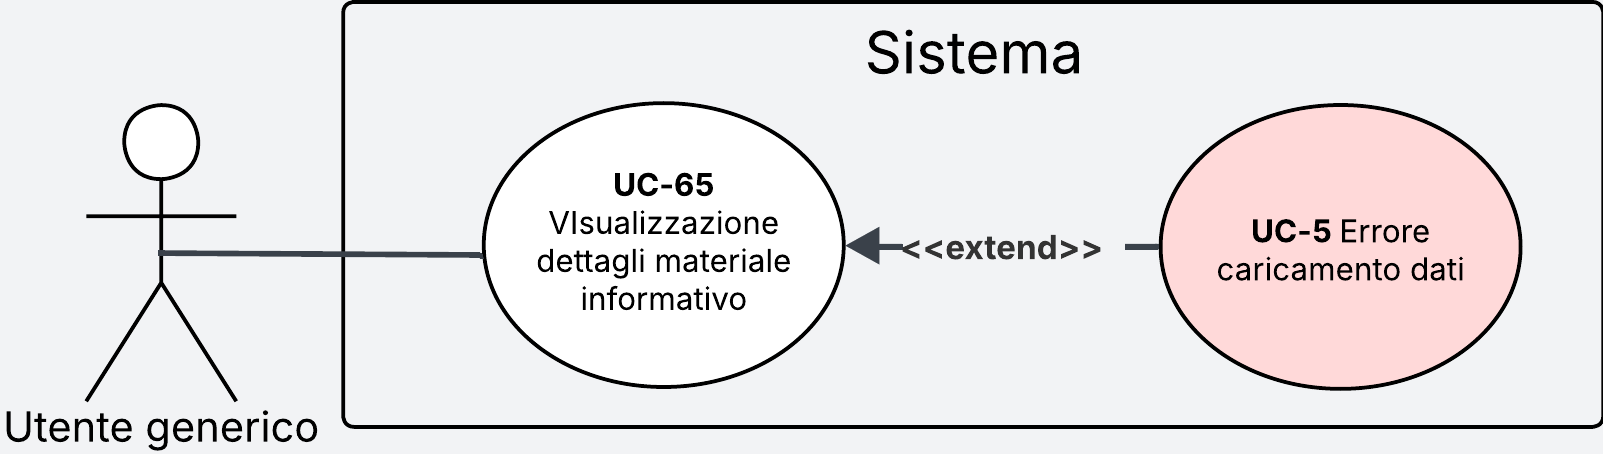
\includegraphics[width=1\textwidth]{use_case/UC-65-coraggio.png}
    \caption{Diagramma del caso d'uso UC-65}
    \label{fig:UC-65}
\end{figure}
\begin{itemize}
    \item \textbf{Attore principale:} \term{Utente} Generico
    \item \textbf{Pre-condizioni:}
    \begin{itemize}
        \item Il sistema è attivo
        \item L'attore visualizza la lista del materiale informativo
    \end{itemize}
    \item \textbf{Post-condizioni:}
    \begin{itemize}
        \item Il contenuto selezionato viene aperto per la consultazione o avviato il download
    \end{itemize}
    \item \textbf{Scenario principale:} 
    \begin{itemize}
        \item L'attore seleziona una risorsa specifica dalla lista
        \item Il sistema recupera il file o il contenuto associato
        \item Il sistema visualizza il materiale a schermo intero o ne avvia la riproduzione
    \end{itemize}
    \item \textbf{Scenario secondario:} 
    \begin{itemize}
         \item Si \ignoreglossary{Verifica} un errore durante il recupero dei dati $\rightarrow$ \hyperref[sec:UC-5]{UC-5}
    \end{itemize}
    \item \textbf{Estensioni:}
     \begin{itemize}
         \item \hyperref[sec:UC-5]{UC-5}
     \end{itemize}
    \item \textbf{Trigger:} L'attore vuole visualizzare i dettagli di una risorsa
\end{itemize}

\subsubsection{UC-66 - Visualizzazione mappa} \label{sec:UC-66}
\begin{figure}[H]
    \centering
    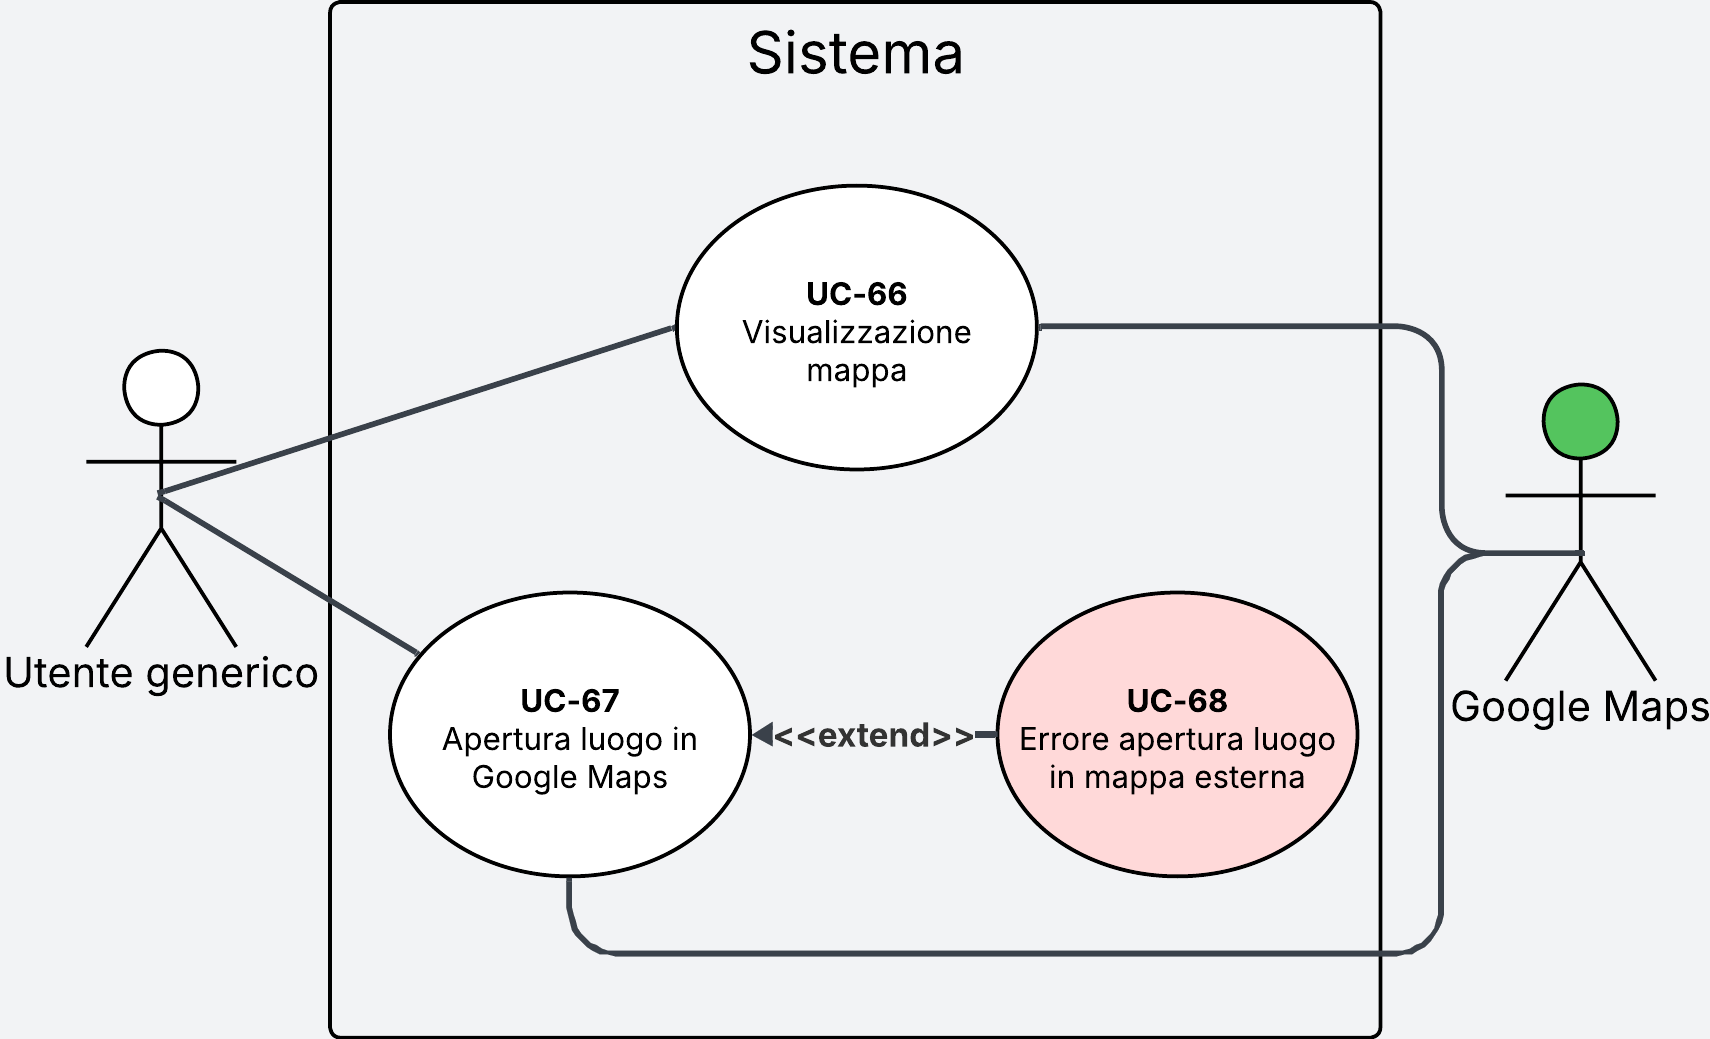
\includegraphics[width=1\textwidth]{use_case/UC-66-67-coraggio.png}
    \caption{Diagramma dei casi d'uso UC-66 e UC-67}
    \label{fig:UC-66}
\end{figure}
\begin{itemize}
    \item \textbf{Attore principale:} \term{Utente} Generico
    \item \textbf{Pre-condizioni:}
    \begin{itemize}
        \item Il sistema è attivo
        \item L'attore ha selezionato la funzionalità per visualizzare la mappa dei luoghi sicuri
    \end{itemize}
    \item \textbf{Post-condizioni:}
    \begin{itemize}
        \item L'attore visualizza la mappa con i punti di interesse
    \end{itemize}
    \item \textbf{Scenario principale:} 
    \begin{itemize}
        \item Il sistema carica i dati geolocalizzati dei luoghi sicuri
        \item Il sistema visualizza la mappa interattiva all'interno dell'applicazione
        \item Il sistema mostra i marker corrispondenti ai luoghi sicuri nelle vicinanze (Centri antiviolenza, Ospedali, Stazioni di Polizia)
    \end{itemize}
    \item \textbf{Trigger:} L'attore vuole localizzare i luoghi sicuri più vicini
\end{itemize}

\subsubsection{UC-67 - Apertura luogo in Google Maps} \label{subsec:UC-67}
\begin{itemize}
    \item \textbf{Attore principale:} \term{Utente} Generico
    \item \textbf{Attore secondario:} Google Maps
    \item \textbf{Pre-condizioni:} 
    \begin{itemize}
        \item Il sistema è attivo
        \item L'attore sta visualizzando la mappa dei luoghi sicuri
        \item Il dispositivo dispone di una connessione internet e/o dell'applicazione Google Maps
    \end{itemize}
    \item \textbf{Post-condizioni:}
    \begin{itemize}
        \item L'applicazione esterna (Google Maps) viene aperta con le coordinate impostate
    \end{itemize}
    \item \textbf{Scenario principale:} 
    \begin{itemize}
        \item L'attore seleziona l'opzione per aprire il luogo su Google Maps
        \item Il sistema chiama l'applicazione esterna Google Maps passando le coordinate necessarie
        \item L'attore Google Maps visualizza la mappa/itinerario
    \end{itemize}
    \item \textbf{Scenario secondario:} 
    \begin{itemize}
         \item Si \ignoreglossary{Verifica} un errore nell'apertura dell'applicazione esterna $\rightarrow$ \hyperref[subsec:UC-68]{UC-68}
    \end{itemize}
    \item \textbf{Estensioni:}
     \begin{itemize}
         \item \hyperref[subsec:UC-68]{UC-68}
     \end{itemize}
    \item \textbf{Trigger:} L'attore vuole avviare la navigazione o vedere dettagli aggiuntivi del luogo
\end{itemize}

\subsubsection{UC-68 - Errore apertura luogo in mappa esterna} \label{subsec:UC-68}
\begin{itemize}
    \item \textbf{Attore principale:} \term{Utente} Generico
    \item \textbf{Pre-condizioni:}
    \begin{itemize}
        \item Il sistema è attivo
        \item Il sistema tenta di aprire l'applicazione Google Maps
        \item Si \ignoreglossary{Verifica} un problema nell'apertura
    \end{itemize}
    \item \textbf{Post-condizioni:}
    \begin{itemize}
        \item Il sistema notifica l'errore e mantiene l'attore nell'applicazione corrente
    \end{itemize}
    \item \textbf{Scenario principale:} 
    \begin{itemize}
        \item Il sistema rileva il fallimento nell'invocazione dell'app esterna
        \item Il sistema mostra un messaggio di errore
        \item Il sistema ritorna alla visualizzazione della mappa interna
    \end{itemize}
    \item \textbf{Trigger:} L'attore vuole tentare di aprire una mappa esterna ma l'operazione fallisce
\end{itemize}

% ======================= REQUISITI ========================

\clearpage
\section{Requisiti} \label{section:requisiti}
Di seguito vengono riportati i requisiti del sistema, individuati attraverso l'analisi dei casi d'uso.
La nomenclatura utilizzata per il codice dei requisiti è spiegata nel documento \href{https://swe-bitbybit.github.io/SWE-docs/docs/RTB/documenti_interni/norme_di_progetto.pdf}{Norme di Progetto} alla sezione 2.2.3.2.

\subsection{Requisiti Funzionali} \label{subsection:requisiti_funzionali}
\begin{center}
\renewcommand{\arraystretch}{1.5}
\arrayrulecolor{black}
\begin{longtable}{|c|p{8.5cm}|>{\centering\arraybackslash}p{4cm}|}

\hline
\rowcolor{gray!60}
\textbf{Codice} & \textbf{Descrizione} & \textbf{Riferimento} \\
\hline
\endfirsthead
\caption[]{Tabella Requisiti Funzionali (continua)} \\
\hline
\rowcolor{gray!60}
\textbf{Codice} & \textbf{Descrizione} & \textbf{Riferimento} \\
\hline
\endhead

\rowcolor{white}
RF-OB-1 & L'\term{Utente} deve poter autenticarsi all'applicazione tramite l'utilizzo di Google Auth & \hyperref[subsec:UC-1]{UC-1} \\
\hline
\rowcolor{gray!20}
RF-OB-2 & Il sistema deve attivare automaticamente la funzionalità di Dead Man's Switch a seguito del login dell'\term{Utente} & \hyperref[subsec:UC-1]{UC-1}, \hyperref[sec:UC-15]{UC-15} \\
\hline
\rowcolor{white}
RF-OB-3 & L'\term{Utente} deve poter visualizzare un messaggio di errore esplicativo nel caso in cui l'autenticazione tramite Google Auth fallisca, venga annullata o restituisca parametri non validi & \hyperref[subsec:UC-2]{UC-2} \\
\hline
\rowcolor{gray!20}
RF-OB-4 & L'\term{Utente} deve poter selezionare il profilo di utilizzo ("Per me" o "Per altri") & \hyperref[subsec:UC-3]{UC-3} \\
\hline
\rowcolor{white}
RF-OB-5 & L'\term{Utente} deve poter visualizzare la lista dei contatti fidati & \hyperref[sec:UC-4]{UC-4} \\
\hline
\rowcolor{gray!20}
RF-OB-6 & L'\term{Utente} deve poter visualizzare un messaggio di errore esplicativo nel caso in cui il recupero dei dati dal database fallisca & \hyperref[sec:UC-5]{UC-5} \\
\hline
\rowcolor{white}
RF-OB-7 & L'\term{Utente} deve poter ricaricare la sezione dei contatti fidati dopo la visualizzazione dell'errore di caricamento dei dati dal database & \hyperref[sec:UC-4]{UC-4}, \hyperref[sec:UC-5]{UC-5} \\
\hline
\rowcolor{gray!20}
RF-OB-8 & Il sistema deve permettere la visualizzazione di un singolo contatto fidato dalla lista dei contatti fidati & \hyperref[subsec:UC-4.1]{UC-4.1} \\
\hline
\rowcolor{white}
RF-OB-9 & L'\term{Utente} deve poter visualizzare la preview delle informazioni (il nome) del contatto fidato che sta visualizzando dalla lista dei contatti fidati & \hyperref[subsec:UC-4.1.1]{UC-4.1.1} \\
\hline
\rowcolor{gray!20}
RF-OB-10 & L'\term{Utente} deve poter visualizzare i dettagli di un contatto fidato selezionato dalla lista dei contatti fidati & \hyperref[subsec:UC-6]{UC-6} \\
\hline
\rowcolor{white}
RF-OB-11 & L'\term{Utente} deve poter visualizzare il nome del contatto fidato selezionato dalla lista dei contatti fidati & \hyperref[subsec:UC-6.1]{UC-6.1} \\
\hline
\rowcolor{gray!20}
RF-OB-12 & L'\term{Utente} deve poter visualizzare il numero di telefono del contatto fidato selezionato dalla lista dei contatti fidati & \hyperref[subsec:UC-6.2]{UC-6.2} \\
\hline
\rowcolor{white}
RF-OB-13 & L'\term{Utente} deve poter visualizzare l'indirizzo email del contatto fidato selezionato dalla lista dei contatti fidati & \hyperref[subsec:UC-6.3]{UC-6.3} \\
\hline
\rowcolor{gray!20}
RF-OB-14 & L'\term{Utente} deve poter aggiungere un nuovo contatto fidato alla lista dei contatti fidati & \hyperref[subsec:UC-7]{UC-7} \\
\hline
\rowcolor{white}
RF-OB-15 & L'\term{Utente} deve poter inserire il nome del nuovo contatto fidato durante l'aggiunta di esso alla lista dei contatti fidati & \hyperref[subsec:UC-7.1]{UC-7.1} \\
\hline
\rowcolor{gray!20}
RF-OB-16 & L'\term{Utente} deve poter inserire il numero di telefono del nuovo contatto fidato durante l'aggiunta di esso alla lista dei contatti fidati & \hyperref[subsec:UC-7.2]{UC-7.2} \\
\hline
\rowcolor{white}
RF-OB-17 & L'\term{Utente} deve poter inserire l'indirizzo email del nuovo contatto fidato durante l'aggiunta di esso alla lista dei contatti fidati & \hyperref[subsec:UC-7.3]{UC-7.3} \\
\hline
\rowcolor{gray!20}
RF-OB-18 & Il sistema deve riconoscere e gestire le informazioni di numero di telefono e email già presenti nel sistema & \hyperref[subsec:UC-9]{UC-9}, \hyperref[subsec:UC-10]{UC-10} \\
\hline
\rowcolor{white}
RF-OB-19 & L'\term{Utente} deve poter visualizzare un messaggio di errore esplicativo nel caso in cui le informazioni di numero di telefono e email siano già presenti nel sistema & \hyperref[subsec:UC-9]{UC-9}, \hyperref[subsec:UC-10]{UC-10} \\
\hline
\rowcolor{gray!20}
RF-OB-20 & L'\term{Utente} deve poter reinserire le informazioni di numero di telefono e email dopo la visualizzazione del messaggio di errore esplicativo & \hyperref[subsec:UC-8]{UC-8}, \hyperref[subsec:UC-9]{UC-9}, \hyperref[subsec:UC-10]{UC-10}, \hyperref[subsec:UC-11]{UC-11} \\
\hline
\rowcolor{white}
RF-OB-21 & Il sistema deve validare la conformità del numero di telefono inserito o modificato & \hyperref[subsec:UC-8]{UC-8}, \hyperref[subsec:UC-7.2]{UC-7.2}, \hyperref[subsec:UC-12.2]{UC-12.2} \\
\hline
\rowcolor{gray!20}
RF-OB-22 & Il sistema deve visualizzare un messaggio di errore esplicativo nel caso in cui il numero di telefono inserito o modificato non sia conforme ai criteri prestabiliti & \hyperref[subsec:UC-8]{UC-8} \\
\hline
\rowcolor{white}
RF-OB-23 & Il sistema deve validare la conformità dell'indirizzo email inserito o modificato & \hyperref[subsec:UC-11]{UC-11}, \hyperref[subsec:UC-7.3]{UC-7.3}, \hyperref[subsec:UC-12.3]{UC-12.3} \\
\hline
\rowcolor{gray!20}
RF-OB-24 & Il sistema deve visualizzare un messaggio di errore esplicativo nel caso in cui l'indirizzo email inserito o modificato non sia conforme ai criteri prestabiliti & \hyperref[subsec:UC-11]{UC-11} \\
\hline
\rowcolor{white}
RF-OB-25 & L'\term{Utente} deve poter modificare i dati di un contatto fidato esistente & \hyperref[subsec:UC-12]{UC-12} \\
\hline
\rowcolor{gray!20}
RF-OB-26 & L'\term{Utente} deve poter modificare il nome di un contatto fidato esistente & \hyperref[subsec:UC-12.1]{UC-12.1} \\
\hline
\rowcolor{white}
RF-OB-27 & L'\term{Utente} deve poter modificare il numero di telefono di un contatto fidato esistente & \hyperref[subsec:UC-12.2]{UC-12.2} \\
\hline
\rowcolor{gray!20}
RF-OB-28 & L'\term{Utente} deve poter modificare l'indirizzo email di un contatto fidato esistente & \hyperref[subsec:UC-12.3]{UC-12.3} \\
\hline
\rowcolor{white}
RF-OB-29 & L'\term{Utente} deve poter eliminare un contatto fidato & \hyperref[subsec:UC-13]{UC-13} \\
\hline
\rowcolor{gray!20}
RF-OB-30 & Il sistema deve richiedere conferma prima dell'eliminazione di un contatto fidato & \hyperref[subsec:UC-13.1]{UC-13.1} \\
\hline
\rowcolor{white}
RF-OB-31 & L'\term{Utente} deve poter confermare, con un'apposita voce, l'eliminazione di un contatto fidato quando il sistema richiede la conferma & \hyperref[subsec:UC-13.1]{UC-13.1} \\
\hline
\rowcolor{gray!20}
RF-OB-32 & L'\term{Utente} deve poter impostare il timer di prima inattività (per la funzionalità di Dead Man's Switch) & \hyperref[sec:UC-15]{UC-15} \\
\hline
\rowcolor{white}
RF-OB-33 & L'\term{Utente} deve poter impostare il timer di seconda inattività (per la funzionalità di Dead Man's Switch) & \hyperref[sec:UC-16]{UC-16} \\
\hline
\rowcolor{gray!20}
RF-OB-34 & L'\term{Utente} deve poter modificare le informazioni della mail di avviso & \hyperref[sec:UC-17]{UC-17} \\
\hline
\rowcolor{white}
RF-OB-35 & L'\term{Utente} deve poter modificare il titolo della mail di avviso & \hyperref[sec:UC-17.1]{UC-17.1} \\
\hline
\rowcolor{gray!20}
RF-OB-36 & L'\term{Utente} deve poter modificare il corpo della mail di avviso & \hyperref[sec:UC-17.2]{UC-17.2} \\
\hline
\rowcolor{white}
RF-OB-37 & L'\term{Utente} deve poter visualizzare un'anteprima della mail di avviso & \hyperref[sec:UC-18]{UC-18} \\
\hline
\rowcolor{gray!20}
RF-OB-38 & L'\term{Utente} deve poter visualizzare l'anteprima del corpo della mail di avviso & \hyperref[subsec:UC-18.1]{UC-18.1} \\
\hline
\rowcolor{white}
RF-OB-39 & L'\term{Utente} deve poter visualizzare un'anteprima del titolo della mail di avviso & \hyperref[subsec:UC-18.2]{UC-18.2} \\
\hline
\rowcolor{gray!20}
RF-OB-40 & L'\term{Utente} deve poter attivare il Dead Man's Switch & \hyperref[sec:UC-19]{UC-19} \\
\hline
\rowcolor{white}
RF-OB-41 & L'\term{Utente} deve poter disattivare la funzionalità di Dead Man's Switch & \hyperref[sec:UC-20]{UC-20} \\
\hline
\rowcolor{gray!20}
RF-OB-42 & L'\term{Utente} deve poter impostare una password per il diario criptato & \hyperref[subsec:UC-21]{UC-21} \\
\hline
\rowcolor{white}
RF-OB-43 & Il sistema deve validare la conformità della password del diario criptato secondo i criteri prestabiliti & \hyperref[subsec:UC-21]{UC-21}, \hyperref[subsec:UC-22]{UC-22} \\
\hline
\rowcolor{gray!20}
RF-OB-44 & Il sistema deve visualizzare un messaggio di errore esplicativo nel caso in cui la password del diario criptato non sia conforme ai criteri prestabiliti & \hyperref[subsec:UC-22]{UC-22} \\
\hline
\rowcolor{white}
RF-OB-45 & L'\term{Utente} deve poter reinserire la password del diario criptato dopo la visualizzazione del messaggio di errore esplicativo & \hyperref[subsec:UC-22]{UC-22} \\
\hline
\rowcolor{gray!20}
RF-OB-46 & L'\term{Utente} deve poter impostare una password per il diario fittizio & \hyperref[subsec:UC-23]{UC-23} \\
\hline
\rowcolor{white}
RF-OB-47 & Il sistema deve validare la conformità e l'unicità della password del diario fittizio rispetto a quella del diario criptato & \hyperref[subsec:UC-22]{UC-22}, \hyperref[subsec:UC-23]{UC-23}, \hyperref[subsec:UC-24]{UC-24} \\
\hline
\rowcolor{gray!20}
RF-OB-48 & Il sistema deve visualizzare un messaggio di errore esplicativo nel caso in cui la password del diario fittizio non sia conforme ai criteri prestabiliti & \hyperref[subsec:UC-22]{UC-22} \\
\hline
\rowcolor{white}
RF-OB-49 & Il sistema deve visualizzare un messaggio di errore esplicativo nel caso in cui la password del diario fittizio sia uguale a quella del diario criptato & \hyperref[subsec:UC-24]{UC-24} \\
\hline
\rowcolor{gray!20}
RF-OB-50 & L'\term{Utente} deve poter reinserire la password del diario fittizio dopo la visualizzazione del messaggio di errore esplicativo & \hyperref[subsec:UC-22]{UC-22}, \hyperref[subsec:UC-24]{UC-24} \\
\hline
\rowcolor{white}
RF-OB-51 & L'\term{Utente} deve poter inserire la password per accedere al diario desiderato & \hyperref[subsec:UC-25]{UC-25} \\
\hline
\rowcolor{gray!20}
RF-OB-52 & L'\term{Utente} deve poter inserire la password per accedere al diario criptato & \hyperref[subsec:UC-25.1]{UC-25.1} \\
\hline
\rowcolor{white}
RF-OB-53 & L'\term{Utente} deve poter inserire la password per accedere al diario fittizio & \hyperref[subsec:UC-25.2]{UC-25.2} \\
\hline
\rowcolor{gray!20}
RF-OB-54 & Il sistema deve visualizzare un messaggio di errore esplicativo nel caso in cui la password inserita per l'accesso al diario risulti errata & \hyperref[subsec:UC-27]{UC-27} \\
\hline
\rowcolor{white}
RF-OB-55 & L'\term{Utente} deve poter reinserire la password di accesso al diario dopo la visualizzazione del messaggio di errore esplicativo & \hyperref[subsec:UC-27]{UC-27} \\
\hline
\rowcolor{gray!20}
RF-OB-56 & Il sistema deve bloccare temporaneamente l'accesso al diario in seguito al superamento del limite massimo di tentativi errati di inserimento password & \hyperref[subsec:UC-26]{UC-26} \\
\hline
\rowcolor{white}
RF-OB-57 & L'\term{Utente} deve poter visualizzare il contenuto del diario criptato & \hyperref[subsec:UC-28]{UC-28} \\
\hline
\rowcolor{gray!20}
RF-OB-58 & L'\term{Utente} deve poter visualizzare la lista delle note presenti nel diario criptato & \hyperref[subsec:UC-28.1]{UC-28.1} \\
\hline
\rowcolor{white}
RF-OB-59 & L'\term{Utente} deve poter visualizzare l'anteprima della singola nota all'interno della lista delle note del diario criptato & \hyperref[subsec:UC-28.1.1]{UC-28.1.1} \\
\hline
\rowcolor{gray!20}
RF-OB-60 & L'\term{Utente} deve poter ricaricare la sezione delle note del diario criptato dopo la visualizzazione dell'errore di caricamento dei dati dal database & \hyperref[subsec:UC-28.1]{UC-28.1}, \hyperref[sec:UC-5]{UC-5} \\
\hline
\rowcolor{white}
RF-OB-61 & L'\term{Utente} deve poter creare una nuova nota vuota all'interno del diario criptato & \hyperref[subsec:UC-31]{UC-31} \\
\hline
\rowcolor{gray!20}
RF-OB-62 & L'\term{Utente} deve poter eliminare una nota esistente dal diario criptato & \hyperref[subsec:UC-30]{UC-30} \\
\hline
\rowcolor{white}
RF-OB-63 & Il sistema deve richiedere conferma prima dell'eliminazione definitiva di una nota del diario criptato & \hyperref[subsec:UC-30.1]{UC-30.1} \\
\hline
\rowcolor{gray!20}
RF-OB-64 & L'\term{Utente} deve poter confermare, con un'apposita voce, l'eliminazione della nota dal diario criptato quando il sistema ne richiede la conferma & \hyperref[subsec:UC-30.1]{UC-30.1} \\
\hline
\rowcolor{white}
RF-OB-65 & L'\term{Utente} deve poter visualizzare il contenuto completo di una nota selezionata dalla lista delle note del diario criptato & \hyperref[subsec:UC-32]{UC-32} \\
\hline
\rowcolor{gray!20}
RF-OB-66 & L'\term{Utente} deve poter visualizzare il contenuto testuale della nota del diario criptato & \hyperref[subsec:UC-32.1]{UC-32.1} \\
\hline
\rowcolor{white}
RF-OB-67 & L'\term{Utente} deve poter visualizzare il contenuto multimediale della nota del diario criptato & \hyperref[subsec:UC-32.2]{UC-32.2} \\
\hline
\rowcolor{gray!20}
RF-OB-68 & L'\term{Utente} deve poter visualizzare il contenuto audio presente all'interno della nota del diario criptato & \hyperref[subsec:UC-32.2.1]{UC-32.2.1} \\
\hline
\rowcolor{white}
RF-OB-69 & L'\term{Utente} deve poter visualizzare le immagini presenti all'interno della nota del diario criptato & \hyperref[subsec:UC-32.2.2]{UC-32.2.2} \\
\hline
\rowcolor{gray!20}
RF-OB-70 & L'\term{Utente} deve poter inserire del contenuto testuale all'interno di una nota del diario criptato & \hyperref[subsec:UC-33]{UC-33} \\
\hline
\rowcolor{white}
RF-OB-71 & L'\term{Utente} deve poter inserire del contenuto multimediale all'interno di una nota del diario criptato & \hyperref[subsec:UC-34]{UC-34} \\
\hline
\rowcolor{gray!20}
RF-OB-72 & L'\term{Utente} deve poter inserire un'immagine all'interno di una nota del diario criptato & \hyperref[subsec:UC-34.1]{UC-34.1} \\
\hline
\rowcolor{white}
RF-OB-73 & L'\term{Utente} deve poter inserire una traccia audio all'interno di una nota del diario criptato & \hyperref[subsec:UC-34.2]{UC-34.2} \\
\hline
\rowcolor{gray!20}
RF-OB-74 & L'\term{Utente} deve poter modificare il contenuto testuale presente all'interno di una nota del diario criptato & \hyperref[subsec:UC-35]{UC-35} \\
\hline
\rowcolor{white}
RF-OB-75 & L'\term{Utente} deve poter rimuovere del contenuto multimediale presente all'interno di una nota del diario criptato & \hyperref[subsec:UC-36]{UC-36} \\
\hline
\rowcolor{gray!20}
RF-OB-76 & L'\term{Utente} deve poter rimuovere un'immagine presente all'interno di una nota del diario criptato & \hyperref[subsec:UC-36.1]{UC-36.1} \\
\hline
\rowcolor{white}
RF-OB-77 & L'\term{Utente} deve poter rimuovere una traccia audio presente all'interno di una nota del diario criptato & \hyperref[subsec:UC-36.2]{UC-36.2} \\
\hline
\rowcolor{gray!20}
RF-OB-78 & L'\term{Utente} deve poter visualizzare la schermata del diario fittizio & \hyperref[subsec:UC-29]{UC-29} \\
\hline
\rowcolor{white}
RF-OB-79 & L'\term{Utente} deve poter visualizzare la lista delle note presenti nel diario fittizio & \hyperref[subsec:UC-29.1]{UC-29.1} \\
\hline
\rowcolor{gray!20}
RF-OB-80 & L'\term{Utente} deve poter visualizzare l'anteprima della singola nota all'interno della lista delle note del diario fittizio & \hyperref[subsec:UC-29.1.1]{UC-29.1.1} \\
\hline
\rowcolor{white}
RF-OB-81 & L'\term{Utente} deve poter ricaricare la sezione delle note del diario fittizio dopo la visualizzazione dell'errore di caricamento dei dati dal database & \hyperref[subsec:UC-29.1]{UC-29.1}, \hyperref[sec:UC-5]{UC-5} \\
\hline
\rowcolor{gray!20}
RF-OB-82 & L'\term{Utente} deve poter eliminare una nota esistente dal diario fittizio & \hyperref[subsec:UC-37]{UC-37} \\
\hline
\rowcolor{white}
RF-OB-83 & Il sistema deve richiedere conferma prima dell'eliminazione definitiva di una nota del diario fittizio & \hyperref[subsec:UC-37.1]{UC-37.1} \\
\hline
\rowcolor{gray!20}
RF-OB-84 & L'\term{Utente} deve poter confermare, con un'apposita voce, l'eliminazione della nota dal diario fittizio quando il sistema ne richiede la conferma & \hyperref[subsec:UC-37.1]{UC-37.1} \\
\hline
\rowcolor{white}
RF-OB-85 & L'\term{Utente} deve poter creare una nuova nota vuota all'interno del diario fittizio & \hyperref[subsec:UC-38]{UC-38} \\
\hline
\rowcolor{gray!20}
RF-OB-86 & L'\term{Utente} deve poter visualizzare il contenuto completo di una nota selezionata dalla lista delle note del diario fittizio & \hyperref[subsec:UC-39]{UC-39} \\
\hline
\rowcolor{white}
RF-OB-87 & L'\term{Utente} deve poter visualizzare il contenuto testuale della nota del diario fittizio & \hyperref[subsec:UC-39.1]{UC-39.1} \\
\hline
\rowcolor{gray!20}
RF-OB-88 & L'\term{Utente} deve poter visualizzare il contenuto multimediale della nota del diario fittizio & \hyperref[subsec:UC-39.2]{UC-39.2} \\
\hline
\rowcolor{white}
RF-OB-89 & L'\term{Utente} deve poter visualizzare il contenuto audio presente all'interno della nota del diario fittizio & \hyperref[subsec:UC-39.2.1]{UC-39.2.1} \\
\hline
\rowcolor{gray!20}
RF-OB-90 & L'\term{Utente} deve poter visualizzare le immagini presenti all'interno della nota del diario fittizio & \hyperref[subsec:UC-39.2.2]{UC-39.2.2} \\
\hline
\rowcolor{white}
RF-OB-91 & L'\term{Utente} deve poter inserire del contenuto testuale all'interno di una nota del diario fittizio & \hyperref[subsec:UC-40]{UC-40} \\
\hline
\rowcolor{gray!20}
RF-OB-92 & L'\term{Utente} deve poter inserire del contenuto multimediale all'interno di una nota del diario fittizio & \hyperref[subsec:UC-41]{UC-41} \\
\hline
\rowcolor{white}
RF-OB-93 & L'\term{Utente} deve poter inserire un'immagine all'interno di una nota del diario fittizio & \hyperref[subsec:UC-41.1]{UC-41.1} \\
\hline
\rowcolor{gray!20}
RF-OB-94 & L'\term{Utente} deve poter inserire una traccia audio all'interno di una nota del diario fittizio & \hyperref[subsec:UC-41.2]{UC-41.2} \\
\hline
\rowcolor{white}
RF-OB-95 & L'\term{Utente} deve poter rimuovere del contenuto multimediale presente all'interno di una nota del diario fittizio & \hyperref[subsec:UC-42]{UC-42} \\
\hline
\rowcolor{gray!20}
RF-OB-96 & L'\term{Utente} deve poter rimuovere un'immagine presente all'interno di una nota del diario fittizio & \hyperref[subsec:UC-42.1]{UC-42.1} \\
\hline
\rowcolor{white}
RF-OB-97 & L'\term{Utente} deve poter rimuovere una traccia audio presente all'interno di una nota del diario fittizio & \hyperref[subsec:UC-42.2]{UC-42.2} \\
\hline
\rowcolor{gray!20}
RF-OB-98 & L'\term{Utente} deve poter modificare il contenuto testuale presente all'interno di una nota del diario fittizio & \hyperref[subsec:UC-43]{UC-43} \\
\hline
\rowcolor{white}
RF-OB-99 & L'\term{Utente} deve poter inviare un messaggio di SOS ai contatti fidati tramite un'apposita voce & \hyperref[sec:UC-44]{UC-44} \\
\hline
\rowcolor{gray!20}
RF-OB-100 & Il sistema deve notificare l'\term{Utente} dell'assenza di connessione internet durante il tentativo di invio del messaggio SOS e proporre l'invio di un segnale acustico & \hyperref[sec:UC-45]{UC-45} \\
\hline
\rowcolor{white}
RF-OB-101 & Il sistema deve notificare l'\term{Utente} della mancanza di contatti fidati configurati durante il tentativo di invio del messaggio SOS e proporre l'invio di un segnale acustico & \hyperref[sec:UC-46]{UC-46} \\
\hline
\rowcolor{gray!20}
RF-OB-102 & L'\term{Utente} deve poter avviare un segnale acustico di emergenza indipendente dalle impostazioni di volume del dispositivo & \hyperref[sec:UC-47]{UC-47} \\
\hline
\rowcolor{white}
RF-OB-103 & L'\term{Utente} deve poter inviare un messaggio al chatbot e ricevere una risposta generata dall'LLM in base al contesto scelto & \hyperref[sec:UC-48]{UC-48} \\
\hline
\rowcolor{gray!20}
RF-OB-104 & L'\term{Utente} deve poter interrompere la generazione della risposta dell'LLM durante la consultazione del chatbot & \hyperref[sec:UC-49]{UC-49} \\
\hline
\rowcolor{white}
RF-OB-105 & Il sistema deve notificare l'\term{Utente} della mancanza di connessione internet durante la consultazione del chatbot & \hyperref[sec:UC-50]{UC-50} \\
\hline
\rowcolor{gray!20}
RF-OB-106 & L'\term{Utente} deve poter ripetere l'invio del messaggio o scriverne uno nuovo dopo la notifica di assenza di connessione internet & \hyperref[sec:UC-50]{UC-50} \\
\hline
\rowcolor{white}
RF-OB-107 & L'\term{Utente} deve poter cambiare il contesto della chat a "Detective delle Relazioni" & \hyperref[sec:UC-51]{UC-51} \\
\hline
\rowcolor{gray!20}
RF-OB-108 & L'\term{Utente} deve poter cambiare il contesto della chat a "Specchio Intelligente" & \hyperref[sec:UC-52]{UC-52} \\
\hline
\rowcolor{white}
RF-OB-109 & Il sistema deve notificare l'\term{Utente} di un errore durante il cambio di contesto del chatbot e mantenere il contesto precedente & \hyperref[sec:UC-53]{UC-53} \\
\hline
\rowcolor{gray!20}
RF-OB-110 & L'\term{Utente} deve poter ritentare il cambio di contesto del chatbot dopo la notifica di errore & \hyperref[sec:UC-53]{UC-53} \\
\hline
\rowcolor{white}
RF-OB-111 & L'\term{Utente} deve poter creare una nuova sessione di chat con il chatbot & \hyperref[subsec:UC-54]{UC-54} \\
\hline
\rowcolor{gray!20}
RF-OB-112 & L'\term{Utente} deve poter eliminare una chat dalla cronologia delle chat & \hyperref[subsec:UC-55]{UC-55} \\
\hline
\rowcolor{white}
RF-OB-113 & Il sistema deve richiedere conferma esplicita prima dell'eliminazione definitiva di una chat & \hyperref[subsec:UC-55.1]{UC-55.1} \\
\hline
\rowcolor{gray!20}
RF-OB-114 & L'\term{Utente} deve poter confermare, con un'apposita voce, l'eliminazione di una chat quando il sistema ne richiede la conferma & \hyperref[subsec:UC-55.1]{UC-55.1} \\
\hline
\rowcolor{white}
RF-OB-115 & L'\term{Utente} deve poter visualizzare il contenuto di una chat selezionata, inclusa la lista dei messaggi scambiati & \hyperref[subsec:UC-56]{UC-56} \\
\hline
\rowcolor{gray!20}
RF-OB-116 & Il sistema deve notificare l'\term{Utente} di un errore nel caricamento del contenuto della chat & \hyperref[sec:UC-5]{UC-5}, \hyperref[subsec:UC-56]{UC-56} \\
\hline
\rowcolor{white}
RF-OB-117 & Il sistema deve visualizzare la lista dei messaggi scambiati tra l'\term{Utente} e il chatbot all'interno di una chat & \hyperref[subsec:UC-56.1]{UC-56.1} \\
\hline
\rowcolor{gray!20}
RF-OB-118 & Il sistema deve distinguere visivamente i messaggi inviati dall'\term{Utente} da quelli generati dal chatbot & \hyperref[subsec:UC-56.1.1]{UC-56.1.1}, \hyperref[subsec:UC-56.1.2]{UC-56.1.2} \\
\hline
\rowcolor{white}
RF-OB-119 & Il sistema deve visualizzare i messaggi inviati dall'\term{Utente} con la formattazione grafica allineata a destra & \hyperref[subsec:UC-56.1.1]{UC-56.1.1} \\
\hline
\rowcolor{gray!20}
RF-OB-120 & Il sistema deve visualizzare i messaggi generati dal chatbot con la formattazione grafica allineata a sinistra & \hyperref[subsec:UC-56.1.2]{UC-56.1.2} \\
\hline
\rowcolor{white}
RF-OB-121 & L'\term{Utente} deve poter visualizzare la cronologia delle chat con il chatbot & \hyperref[subsec:UC-57]{UC-57} \\
\hline
\rowcolor{gray!20}
RF-OB-122 & L'\term{Utente} deve poter selezionare e visualizzare una singola chat dalla cronologia & \hyperref[subsec:UC-57.1]{UC-57.1} \\
\hline
\rowcolor{white}
RF-OB-123 & Il sistema deve mostrare il titolo identificativo di ogni chat presente nella cronologia & \hyperref[subsec:UC-57.1.1]{UC-57.1.1} \\
\hline
\rowcolor{gray!20}
RF-OB-124 & L'\term{Utente} deve poter visualizzare la lista delle community disponibili & \hyperref[sec:UC-58]{UC-58} \\
\hline
\rowcolor{white}
RF-OB-125 & Il sistema deve notificare l'\term{Utente} di un errore nel caricamento della lista delle community & \hyperref[sec:UC-5]{UC-5}, \hyperref[sec:UC-58]{UC-58} \\
\hline
\rowcolor{gray!20}
RF-OB-126 & Il sistema deve mostrare i dati riassuntivi di ogni singola community nella lista & \hyperref[subsec:UC-58.1]{UC-58.1} \\
\hline
\rowcolor{white}
RF-OB-127 & Il sistema deve mostrare il nome di ogni singola community nella lista & \hyperref[subsec:UC-58.1.1]{UC-58.1.1} \\
\hline
\rowcolor{gray!20}
RF-OB-128 & Il sistema deve mostrare il link di ogni singola community nella lista & \hyperref[subsec:UC-58.1.2]{UC-58.1.2} \\
\hline
\rowcolor{white}
RF-OB-129 & L'\term{Utente} deve poter aprire il link di una community per visitarne il sito web esterno & \hyperref[sec:UC-59]{UC-59} \\
\hline
\rowcolor{gray!20}
RF-OB-130 & L'\term{Utente} deve poter visualizzare la lista delle leggi e normative disponibili & \hyperref[sec:UC-60]{UC-60} \\
\hline
\rowcolor{white}
RF-OB-131 & Il sistema deve mostrare il titolo di ogni singola legge nella lista & \hyperref[subsec:UC-60.1]{UC-60.1} \\
\hline
\rowcolor{gray!20}
RF-OB-132 & L'\term{Utente} deve poter visualizzare i dettagli completi di una legge selezionata dalla lista & \hyperref[sec:UC-61]{UC-61} \\
\hline
\rowcolor{white}
RF-OB-133 & Il sistema deve notificare l'\term{Utente} di un errore nel caricamento dei dati di una legge & \hyperref[sec:UC-5]{UC-5}, \hyperref[sec:UC-61]{UC-61} \\
\hline
\rowcolor{gray!20}
RF-OB-134 & L'\term{Utente} deve poter visualizzare la lista dei contatti e degli enti d'emergenza & \hyperref[sec:UC-62]{UC-62} \\
\hline
\rowcolor{white}
RF-OB-135 & Il sistema deve mostrare i dati riassuntivi di ogni singolo contatto d'emergenza nella lista & \hyperref[subsec:UC-62.1]{UC-62.1} \\
\hline
\rowcolor{gray!20}
RF-OB-136 & Il sistema deve mostrare il nome identificativo di ogni contatto d'emergenza & \hyperref[subsec:UC-62.1.1]{UC-62.1.1} \\
\hline
\rowcolor{white}
RF-OB-137 & Il sistema deve mostrare il numero di telefono associato ad ogni contatto d'emergenza & \hyperref[subsec:UC-62.1.2]{UC-62.1.2} \\
\hline
\rowcolor{gray!20}
RF-OB-138 & L'\term{Utente} deve poter comporre automaticamente il numero di un contatto d'emergenza tramite l'apposita voce & \hyperref[sec:UC-63]{UC-63} \\
\hline
\rowcolor{white}
RF-OB-139 & L'\term{Utente} deve poter visualizzare la lista del materiale informativo disponibile & \hyperref[sec:UC-64]{UC-64} \\
\hline
\rowcolor{gray!20}
RF-OB-140 & Il sistema deve notificare l'\term{Utente} di un errore nel caricamento della lista del materiale informativo & \hyperref[sec:UC-5]{UC-5}, \hyperref[sec:UC-64]{UC-64} \\
\hline
\rowcolor{white}
RF-OB-141 & Il sistema deve mostrare il titolo e il formato di ogni singolo materiale informativo nella lista & \hyperref[subsec:UC-64.1]{UC-64.1} \\
\hline
\rowcolor{gray!20}
RF-OB-142 & L'\term{Utente} deve poter visualizzare il contenuto di un materiale informativo selezionato dalla lista & \hyperref[sec:UC-65]{UC-65} \\
\hline
\rowcolor{white}
RF-OB-143 & Il sistema deve notificare l'\term{Utente} di un errore nel recupero dei dati del materiale informativo & \hyperref[sec:UC-5]{UC-5}, \hyperref[sec:UC-65]{UC-65} \\
\hline
\rowcolor{gray!20}
RF-OB-144 & L'\term{Utente} deve poter visualizzare la mappa interattiva con i marker dei luoghi sicuri nelle vicinanze & \hyperref[sec:UC-66]{UC-66} \\
\hline
\rowcolor{white}
RF-OB-145 & L'\term{Utente} deve poter aprire un luogo sicuro nella mappa esterna Google Maps & \hyperref[subsec:UC-67]{UC-67} \\
\hline
\rowcolor{gray!20}
RF-OB-146 & Il sistema deve notificare l'\term{Utente} di un errore nell'apertura dell'applicazione Google Maps e mantenere la visualizzazione della mappa interna & \hyperref[subsec:UC-68]{UC-68} \\
\hline
\caption{Tabella Requisiti Funzionali} \label{tab:requisiti_funzionali} \\
\end{longtable}
\end{center}

\subsection{Requisiti di Qualità} \label{subsection:requisiti_qualita}
\begin{center}
\renewcommand{\arraystretch}{1.5}
\arrayrulecolor{black}
\begin{longtable}{|c|p{8.5cm}|>{\centering\arraybackslash}p{4cm}|}
\hline
\rowcolor{gray!60}
\textbf{Codice} & \textbf{Descrizione} & \textbf{Riferimento} \\
\hline
\endfirsthead
\caption[]{Tabella Requisiti di Qualità (continua)} \\
\hline
\rowcolor{gray!60}
\textbf{Codice} & \textbf{Descrizione} & \textbf{Riferimento} \\
\hline
\endhead
\rowcolor{white}
RQ-OB-1 & Il \term{Processo} di sviluppo del software deve prevedere un'attività di \term{Verifica} continua tramite la stesura e l'esecuzione di \term{Test Di Unità} per ogni componente implementato & \term{Capitolato} d'appalto \href{https://www.math.unipd.it/~tullio/IS-1/2025/Progetto/C4.pdf}{Capitolato} \\
\hline
\rowcolor{gray!20}
RQ-OB-2 & Le verifiche effettuate, le misurazioni sui test e i relativi risultati devono essere tracciati sistematicamente all'interno del documento \term{Piano Di Qualifica} & Decisione interna \href{https://swe-bitbybit.github.io/SWE-docs/docs/RTB/documenti_esterni/piano_di_qualifica.pdf}{Piano di Qualifica} \\
\hline
\rowcolor{white}
RQ-OB-3 & Tutte le attività del \term{Ciclo Di Vita} del prodotto (efficienza dei processi, convenzioni di codifica e stesura) devono conformarsi a quanto regolamentato dalle Norme di Progetto & Decisione interna \href{https://swe-bitbybit.github.io/SWE-docs/docs/RTB/documenti_interni/norme_di_progetto.pdf}{Norme di Progetto} \\
\hline
\rowcolor{gray!20}
RQ-OB-4 & Il \term{Processo} di tracciamento e versionamento per tutto il materiale di progetto, deve appoggiarsi al software Git e alla piattaforma GitHub & Decisione interna \href{https://swe-bitbybit.github.io/SWE-docs/docs/RTB/documenti_interni/norme_di_progetto.pdf}{Norme di Progetto} \\
\hline
\rowcolor{white}
RQ-OB-5 & Il monitoraggio della qualità del software deve basarsi sul calcolo strutturato di metriche statiche e dinamiche, le cui soglie sono stabilite nel \term{Piano Di Qualifica} & Decisione interna \href{https://swe-bitbybit.github.io/SWE-docs/docs/RTB/documenti_esterni/piano_di_qualifica.pdf}{Piano di Qualifica} \\
\hline
\rowcolor{gray!20}
RQ-OB-6 & Le procedure di controllo continuo sul materiale prodotto (come compilazione e analisi della qualità del codice) devono essere automatizzate mediante l'uso di una pipeline di Continuous Integration (\term{Github Actions}) & Decisione interna \href{https://swe-bitbybit.github.io/SWE-docs/docs/RTB/documenti_interni/norme_di_progetto.pdf}{Norme di Progetto} \\
\hline
\rowcolor{white}
RQ-OB-7 & L'assegnazione e l'avanzamento delle attività \term{To-Do} e la progressione complessiva del lavoro devono essere guidate da un'opportuna pianificazione basata su un sistema di \term{Issue} Tracking (GitHub Projects) & Decisione interna \href{https://swe-bitbybit.github.io/SWE-docs/docs/RTB/documenti_interni/norme_di_progetto.pdf}{Norme di Progetto} \\
\hline
\rowcolor{gray!20}
RQ-OB-8 & L'intera documentazione formale di progetto deve essere redatta esclusivamente formattandola tramite il linguaggio di markup tipografico \LaTeX & Decisione interna \href{https://swe-bitbybit.github.io/SWE-docs/docs/RTB/documenti_interni/norme_di_progetto.pdf}{Norme di Progetto} \\
\hline
\caption{Tabella Requisiti di Qualità} \label{tab:requisiti_qualita} \\
\end{longtable}
\end{center}

\subsection{Requisiti di Vincolo} \label{subsection:requisiti_vincolo}
\begin{center}
\renewcommand{\arraystretch}{1.5}
\arrayrulecolor{black}
\begin{longtable}{|c|p{8.5cm}|>{\centering\arraybackslash}p{4cm}|}

\hline
\rowcolor{gray!60}
\textbf{Codice} & \textbf{Descrizione} & \textbf{Riferimento} \\
\hline
\endfirsthead
\caption[]{Tabella Requisiti di Vincolo (continua)} \\
\hline
\rowcolor{gray!60}
\textbf{Codice} & \textbf{Descrizione} & \textbf{Riferimento} \\
\hline
\endhead
\rowcolor{white}
RV-OB-1 & L'applicazione client deve garantire piena compatibilità con il sistema operativo Android, a partire dalla versione 8.0 (API 26) & \href{https://www.math.unipd.it/~tullio/IS-1/2025/Progetto/C4.pdf}{Capitolato} \newline Sez. 3.4 \\
\hline
\rowcolor{gray!20}
RV-OB-2 & L'applicazione client deve garantire piena compatibilità con il sistema operativo iOS, a partire dalla versione 15.0 & \href{https://www.math.unipd.it/~tullio/IS-1/2025/Progetto/C4.pdf}{Capitolato} \newline Sez. 3.4 \\
\hline
\rowcolor{white}
RV-OB-3 & Lo sviluppo dell'applicazione mobile e dell'interfaccia \term{Utente} deve essere condotto impiegando il framework cross-platform Flutter & \href{https://www.math.unipd.it/~tullio/IS-1/2025/Progetto/C4.pdf}{Capitolato} \newline Sez. 3.4 \\
\hline
\rowcolor{gray!20}
RV-OB-4 & L'infrastruttura di backend del sistema deve essere ospitata su servizi Cloud scalabili e sicuri, avvalendosi specificatamente del provider Amazon Web Services (AWS) & \href{https://www.math.unipd.it/~tullio/IS-1/2025/Progetto/C4.pdf}{Capitolato} \newline Sez. 3.4 \\
\hline
\rowcolor{white}
RV-OB-5 & L'\term{Architettura} del backend deve basarsi su un modello a microservizi di tipo Serverless, avvalendosi dell'esecuzione di funzioni AWS Lambda & \href{https://www.math.unipd.it/~tullio/IS-1/2025/Progetto/C4.pdf}{Capitolato} \newline Sez. 3.2 \\
\hline
\rowcolor{gray!20}
RV-OB-6 & Le comunicazioni telematiche tra l'applicazione mobile (frontend) e i microservizi di backend devono avvenire in modo sicuro tramite Amazon API Gateway & \href{https://www.math.unipd.it/~tullio/IS-1/2025/Progetto/C4.pdf}{Capitolato} \newline Sez. 3.4 \\
\hline
\rowcolor{white}
RV-OB-7 & La persistenza ed organizzazione dei dati applicativi deve appoggiarsi su database adeguatamente scalabili e resilienti, prediligendo un approccio NoSQL gestito tramite Amazon DynamoDB & \href{https://www.math.unipd.it/~tullio/IS-1/2025/Progetto/C4.pdf}{Capitolato} \newline Sez. 3.4 \\
\hline
\rowcolor{gray!20}
RV-OB-8 & I meccanismi di sicurezza, registrazione e autenticazione forte degli utenti (autorizzazione granulare) previsti dal progetto devono essere garantiti tramite l'adozione attiva di Amazon Cognito & \href{https://www.math.unipd.it/~tullio/IS-1/2025/Progetto/C4.pdf}{Capitolato} \newline Sez. 3.1 \\
\hline
\rowcolor{white}
RV-OB-9 & L'integrazione delle funzionalità di Intelligenza Artificiale Generativa e l'utilizzo dei modelli fondazionali (LLM) devono avvenire esclusivamente tramite il servizio Amazon Bedrock & Decisione interna \\
\hline
\rowcolor{gray!20}
RV-OB-10 & L'interfaccia \ignoreglossary{utente} deve essere utilizzabile senza perdita di funzionalità ed adattarsi dinamicamente alle seguenti dimensioni di schermo: 360 px (smartphone portrait), 640 px (smartphone landscape), 768 px (tablet portrait) e 1024 px (tablet landscape) & \href{https://www.math.unipd.it/~tullio/IS-1/2025/Progetto/C4.pdf}{Capitolato} \newline Sez. 3.4 \\
\hline
\rowcolor{white}
RV-OB-11 & L'infrastruttura cloud del sistema deve essere configurata in modo da supportare l'alta disponibilità, delegando la resilienza dell'infrastruttura ai servizi gestiti AWS & Decisione interna; Decisione Esterna \\
\hline
\caption{Tabella Requisiti di Vincolo} \label{tab:requisiti_vincolo} \\
\end{longtable}
\end{center}

\subsection{Tracciamento dei casi d'uso} \label{subsection:tracciamento_uc}
\begin{center}
\renewcommand{\arraystretch}{1.5}
\arrayrulecolor{black}
\begin{longtable}{|>{\centering\arraybackslash}p{5cm}|>{\centering\arraybackslash}p{9cm}|}

\hline
\rowcolor{gray!60}
\textbf{Caso d'Uso} & \textbf{Requisiti} \\
\hline
\endfirsthead
\caption[]{Tracciamento dei casi d'uso (continua)} \\
\hline
\rowcolor{gray!60}
\textbf{Caso d'Uso} & \textbf{Requisiti} \\
\hline
\endhead
\rowcolor{white}
\hyperref[subsec:UC-1]{UC-1} & RF-OB-1, RF-OB-2 \\
\hline
\rowcolor{gray!20}
\hyperref[subsec:UC-2]{UC-2} & RF-OB-3 \\
\hline
\rowcolor{white}
\hyperref[subsec:UC-3]{UC-3} & RF-OB-4 \\
\hline
\rowcolor{gray!20}
\hyperref[sec:UC-4]{UC-4} & RF-OB-5, RF-OB-7 \\
\hline
\rowcolor{white}
\hyperref[subsec:UC-4.1]{UC-4.1} & RF-OB-8 \\
\hline
\rowcolor{gray!20}
\hyperref[subsec:UC-4.1.1]{UC-4.1.1} & RF-OB-9 \\
\hline
\rowcolor{white}
\hyperref[sec:UC-5]{UC-5} & RF-OB-6, RF-OB-7, RF-OB-60, RF-OB-81, RF-OB-116, RF-OB-125, RF-OB-133, RF-OB-140, RF-OB-143 \\
\hline
\rowcolor{gray!20}
\hyperref[subsec:UC-6]{UC-6} & RF-OB-10 \\
\hline
\rowcolor{white}
\hyperref[subsec:UC-6.1]{UC-6.1} & RF-OB-11 \\
\hline
\rowcolor{gray!20}
\hyperref[subsec:UC-6.2]{UC-6.2} & RF-OB-12 \\
\hline
\rowcolor{white}
\hyperref[subsec:UC-6.3]{UC-6.3} & RF-OB-13 \\
\hline
\rowcolor{gray!20}
\hyperref[subsec:UC-7]{UC-7} & RF-OB-14 \\
\hline
\rowcolor{white}
\hyperref[subsec:UC-7.1]{UC-7.1} & RF-OB-15 \\
\hline
\rowcolor{gray!20}
\hyperref[subsec:UC-7.2]{UC-7.2} & RF-OB-16, RF-OB-21 \\
\hline
\rowcolor{white}
\hyperref[subsec:UC-7.3]{UC-7.3} & RF-OB-17, RF-OB-23 \\
\hline
\rowcolor{gray!20}
\hyperref[subsec:UC-8]{UC-8} & RF-OB-20, RF-OB-21, RF-OB-22 \\
\hline
\rowcolor{white}
\hyperref[subsec:UC-9]{UC-9} & RF-OB-18, RF-OB-19, RF-OB-20 \\
\hline
\rowcolor{gray!20}
\hyperref[subsec:UC-10]{UC-10} & RF-OB-18, RF-OB-19, RF-OB-20 \\
\hline
\rowcolor{white}
\hyperref[subsec:UC-11]{UC-11} & RF-OB-20, RF-OB-23, RF-OB-24 \\
\hline
\rowcolor{gray!20}
\hyperref[subsec:UC-12]{UC-12} & RF-OB-25 \\
\hline
\rowcolor{white}
\hyperref[subsec:UC-12.1]{UC-12.1} & RF-OB-26 \\
\hline
\rowcolor{gray!20}
\hyperref[subsec:UC-12.2]{UC-12.2} & RF-OB-27, RF-OB-21 \\
\hline
\rowcolor{white}
\hyperref[subsec:UC-12.3]{UC-12.3} & RF-OB-28, RF-OB-23 \\
\hline
\rowcolor{gray!20}
\hyperref[subsec:UC-13]{UC-13} & RF-OB-29 \\
\hline
\rowcolor{white}
\hyperref[subsec:UC-13.1]{UC-13.1} & RF-OB-30, RF-OB-31 \\
\hline
\rowcolor{gray!20}
\hyperref[sec:UC-15]{UC-15} & RF-OB-2, RF-OB-32 \\
\hline
\rowcolor{white}
\hyperref[sec:UC-16]{UC-16} & RF-OB-33 \\
\hline
\rowcolor{gray!20}
\hyperref[sec:UC-17]{UC-17} & RF-OB-34 \\
\hline
\rowcolor{white}
\hyperref[sec:UC-17.1]{UC-17.1} & RF-OB-35 \\
\hline
\rowcolor{gray!20}
\hyperref[sec:UC-17.2]{UC-17.2} & RF-OB-36 \\
\hline
\rowcolor{white}
\hyperref[sec:UC-18]{UC-18} & RF-OB-37 \\
\hline
\rowcolor{gray!20}
\hyperref[subsec:UC-18.1]{UC-18.1} & RF-OB-38 \\
\hline
\rowcolor{white}
\hyperref[subsec:UC-18.2]{UC-18.2} & RF-OB-39 \\
\hline
\rowcolor{gray!20}
\hyperref[sec:UC-19]{UC-19} & RF-OB-40 \\
\hline
\rowcolor{white}
\hyperref[sec:UC-20]{UC-20} & RF-OB-41 \\
\hline
\rowcolor{gray!20}
\hyperref[subsec:UC-21]{UC-21} & RF-OB-42, RF-OB-43 \\
\hline
\rowcolor{white}
\hyperref[subsec:UC-22]{UC-22} & RF-OB-43, RF-OB-44, RF-OB-45, RF-OB-47, RF-OB-48, RF-OB-50 \\
\hline
\rowcolor{gray!20}
\hyperref[subsec:UC-23]{UC-23} & RF-OB-46, RF-OB-47 \\
\hline
\rowcolor{white}
\hyperref[subsec:UC-24]{UC-24} & RF-OB-47, RF-OB-49, RF-OB-50 \\
\hline
\rowcolor{gray!20}
\hyperref[subsec:UC-25]{UC-25} & RF-OB-51 \\
\hline
\rowcolor{white}
\hyperref[subsec:UC-25.1]{UC-25.1} & RF-OB-52 \\
\hline
\rowcolor{gray!20}
\hyperref[subsec:UC-25.2]{UC-25.2} & RF-OB-53 \\
\hline
\rowcolor{white}
\hyperref[subsec:UC-26]{UC-26} & RF-OB-56 \\
\hline
\rowcolor{gray!20}
\hyperref[subsec:UC-27]{UC-27} & RF-OB-54, RF-OB-55 \\
\hline
\rowcolor{white}
\hyperref[subsec:UC-28]{UC-28} & RF-OB-57 \\
\hline
\rowcolor{gray!20}
\hyperref[subsec:UC-28.1]{UC-28.1} & RF-OB-58, RF-OB-60 \\
\hline
\rowcolor{white}
\hyperref[subsec:UC-28.1.1]{UC-28.1.1} & RF-OB-59 \\
\hline
\rowcolor{gray!20}
\hyperref[subsec:UC-29]{UC-29} & RF-OB-78 \\
\hline
\rowcolor{white}
\hyperref[subsec:UC-29.1]{UC-29.1} & RF-OB-79, RF-OB-81 \\
\hline
\rowcolor{gray!20}
\hyperref[subsec:UC-29.1.1]{UC-29.1.1} & RF-OB-80 \\
\hline
\rowcolor{white}
\hyperref[subsec:UC-30]{UC-30} & RF-OB-62 \\
\hline
\rowcolor{gray!20}
\hyperref[subsec:UC-30.1]{UC-30.1} & RF-OB-63, RF-OB-64 \\
\hline
\rowcolor{white}
\hyperref[subsec:UC-31]{UC-31} & RF-OB-61 \\
\hline
\rowcolor{gray!20}
\hyperref[subsec:UC-32]{UC-32} & RF-OB-65 \\
\hline
\rowcolor{white}
\hyperref[subsec:UC-32.1]{UC-32.1} & RF-OB-66 \\
\hline
\rowcolor{gray!20}
\hyperref[subsec:UC-32.2]{UC-32.2} & RF-OB-67 \\
\hline
\rowcolor{white}
\hyperref[subsec:UC-32.2.1]{UC-32.2.1} & RF-OB-68 \\
\hline
\rowcolor{gray!20}
\hyperref[subsec:UC-32.2.2]{UC-32.2.2} & RF-OB-69 \\
\hline
\rowcolor{white}
\hyperref[subsec:UC-33]{UC-33} & RF-OB-70 \\
\hline
\rowcolor{gray!20}
\hyperref[subsec:UC-34]{UC-34} & RF-OB-71 \\
\hline
\rowcolor{white}
\hyperref[subsec:UC-34.1]{UC-34.1} & RF-OB-72 \\
\hline
\rowcolor{gray!20}
\hyperref[subsec:UC-34.2]{UC-34.2} & RF-OB-73 \\
\hline
\rowcolor{white}
\hyperref[subsec:UC-35]{UC-35} & RF-OB-74 \\
\hline
\rowcolor{gray!20}
\hyperref[subsec:UC-36]{UC-36} & RF-OB-75 \\
\hline
\rowcolor{white}
\hyperref[subsec:UC-36.1]{UC-36.1} & RF-OB-76 \\
\hline
\rowcolor{gray!20}
\hyperref[subsec:UC-36.2]{UC-36.2} & RF-OB-77 \\
\hline
\rowcolor{white}
\hyperref[subsec:UC-37]{UC-37} & RF-OB-82 \\
\hline
\rowcolor{gray!20}
\hyperref[subsec:UC-37.1]{UC-37.1} & RF-OB-83, RF-OB-84 \\
\hline
\rowcolor{white}
\hyperref[subsec:UC-38]{UC-38} & RF-OB-85 \\
\hline
\rowcolor{gray!20}
\hyperref[subsec:UC-39]{UC-39} & RF-OB-86 \\
\hline
\rowcolor{white}
\hyperref[subsec:UC-39.1]{UC-39.1} & RF-OB-87 \\
\hline
\rowcolor{gray!20}
\hyperref[subsec:UC-39.2]{UC-39.2} & RF-OB-88 \\
\hline
\rowcolor{white}
\hyperref[subsec:UC-39.2.1]{UC-39.2.1} & RF-OB-89 \\
\hline
\rowcolor{gray!20}
\hyperref[subsec:UC-39.2.2]{UC-39.2.2} & RF-OB-90 \\
\hline
\rowcolor{white}
\hyperref[subsec:UC-40]{UC-40} & RF-OB-91 \\
\hline
\rowcolor{gray!20}
\hyperref[subsec:UC-41]{UC-41} & RF-OB-92 \\
\hline
\rowcolor{white}
\hyperref[subsec:UC-41.1]{UC-41.1} & RF-OB-93 \\
\hline
\rowcolor{gray!20}
\hyperref[subsec:UC-41.2]{UC-41.2} & RF-OB-94 \\
\hline
\rowcolor{white}
\hyperref[subsec:UC-42]{UC-42} & RF-OB-95 \\
\hline
\rowcolor{gray!20}
\hyperref[subsec:UC-42.1]{UC-42.1} & RF-OB-96 \\
\hline
\rowcolor{white}
\hyperref[subsec:UC-42.2]{UC-42.2} & RF-OB-97 \\
\hline
\rowcolor{gray!20}
\hyperref[subsec:UC-43]{UC-43} & RF-OB-98 \\
\hline
\rowcolor{white}
\hyperref[sec:UC-44]{UC-44} & RF-OB-99 \\
\hline
\rowcolor{gray!20}
\hyperref[sec:UC-45]{UC-45} & RF-OB-100 \\
\hline
\rowcolor{white}
\hyperref[sec:UC-46]{UC-46} & RF-OB-101 \\
\hline
\rowcolor{gray!20}
\hyperref[sec:UC-47]{UC-47} & RF-OB-102 \\
\hline
\rowcolor{white}
\hyperref[sec:UC-48]{UC-48} & RF-OB-103 \\
\hline
\rowcolor{gray!20}
\hyperref[sec:UC-49]{UC-49} & RF-OB-104 \\
\hline
\rowcolor{white}
\hyperref[sec:UC-50]{UC-50} & RF-OB-105, RF-OB-106 \\
\hline
\rowcolor{gray!20}
\hyperref[sec:UC-51]{UC-51} & RF-OB-107 \\
\hline
\rowcolor{white}
\hyperref[sec:UC-52]{UC-52} & RF-OB-108 \\
\hline
\rowcolor{gray!20}
\hyperref[sec:UC-53]{UC-53} & RF-OB-109, RF-OB-110 \\
\hline
\rowcolor{white}
\hyperref[subsec:UC-54]{UC-54} & RF-OB-111 \\
\hline
\rowcolor{gray!20}
\hyperref[subsec:UC-55]{UC-55} & RF-OB-112 \\
\hline
\rowcolor{white}
\hyperref[subsec:UC-55.1]{UC-55.1} & RF-OB-113, RF-OB-114 \\
\hline
\rowcolor{gray!20}
\hyperref[subsec:UC-56]{UC-56} & RF-OB-115, RF-OB-116 \\
\hline
\rowcolor{white}
\hyperref[subsec:UC-56.1]{UC-56.1} & RF-OB-117 \\
\hline
\rowcolor{gray!20}
\hyperref[subsec:UC-56.1.1]{UC-56.1.1} & RF-OB-118, RF-OB-119 \\
\hline
\rowcolor{white}
\hyperref[subsec:UC-56.1.2]{UC-56.1.2} & RF-OB-118, RF-OB-120 \\
\hline
\rowcolor{gray!20}
\hyperref[subsec:UC-57]{UC-57} & RF-OB-121 \\
\hline
\rowcolor{white}
\hyperref[subsec:UC-57.1]{UC-57.1} & RF-OB-122 \\
\hline
\rowcolor{gray!20}
\hyperref[subsec:UC-57.1.1]{UC-57.1.1} & RF-OB-123 \\
\hline
\rowcolor{white}
\hyperref[sec:UC-58]{UC-58} & RF-OB-124, RF-OB-125 \\
\hline
\rowcolor{gray!20}
\hyperref[subsec:UC-58.1]{UC-58.1} & RF-OB-126 \\
\hline
\rowcolor{white}
\hyperref[subsec:UC-58.1.1]{UC-58.1.1} & RF-OB-127 \\
\hline
\rowcolor{gray!20}
\hyperref[subsec:UC-58.1.2]{UC-58.1.2} & RF-OB-128 \\
\hline
\rowcolor{white}
\hyperref[sec:UC-59]{UC-59} & RF-OB-129 \\
\hline
\rowcolor{gray!20}
\hyperref[sec:UC-60]{UC-60} & RF-OB-130 \\
\hline
\rowcolor{white}
\hyperref[subsec:UC-60.1]{UC-60.1} & RF-OB-131 \\
\hline
\rowcolor{gray!20}
\hyperref[sec:UC-61]{UC-61} & RF-OB-132, RF-OB-133 \\
\hline
\rowcolor{white}
\hyperref[sec:UC-62]{UC-62} & RF-OB-134 \\
\hline
\rowcolor{gray!20}
\hyperref[subsec:UC-62.1]{UC-62.1} & RF-OB-135 \\
\hline
\rowcolor{white}
\hyperref[subsec:UC-62.1.1]{UC-62.1.1} & RF-OB-136 \\
\hline
\rowcolor{gray!20}
\hyperref[subsec:UC-62.1.2]{UC-62.1.2} & RF-OB-137 \\
\hline
\rowcolor{white}
\hyperref[sec:UC-63]{UC-63} & RF-OB-138 \\
\hline
\rowcolor{gray!20}
\hyperref[sec:UC-64]{UC-64} & RF-OB-139, RF-OB-140 \\
\hline
\rowcolor{white}
\hyperref[subsec:UC-64.1]{UC-64.1} & RF-OB-141 \\
\hline
\rowcolor{gray!20}
\hyperref[sec:UC-65]{UC-65} & RF-OB-142, RF-OB-143 \\
\hline
\rowcolor{white}
\hyperref[sec:UC-66]{UC-66} & RF-OB-144 \\
\hline
\rowcolor{gray!20}
\hyperref[subsec:UC-67]{UC-67} & RF-OB-145 \\
\hline
\rowcolor{white}
\hyperref[subsec:UC-68]{UC-68} & RF-OB-146 \\
\hline
\caption{Tracciamento dei casi d'uso} \label{tab:tracciamento_uc} \\
\end{longtable}
\end{center}

\end{document}